\mychapter{Singular Integrals}\label{ch4}

\section{Maximal functions}\label{ch4_sec1}

\subsecbkm{ch4_sec1.1}{Formulation}

Let $Z_t$ be a Brownian motion in $\R^2$, let $u$ be a function that is harmonic in the upper half-plane, and let $v$ be the conjugate harmonic function to $u$. The basic connection between Brownian motion and singular integrals comes about through the observation that $v(Z_t)$ is a martingale transform of $u(Z_t)$. In this chapter we will exploit this relationship and similar ones to obtain many results about the Hilbert transform, Riesz transform, Littlewood-Paley functionals, and other singular integrals.

This section contains some basic properties of the maximal function. Certain of these results are consequences of what was proved in Chap.\ \ref{ch3}, but here the derivation is much more direct.

In this section we will be working in the half-space $D = \R^d \times [0,\infty)$. We will denote elements of $D$ by $z = (x,y)$ with $x \in \R^d$, $y \in [0,\infty)$. Let $X_t$ be a $d$-dimensional Brownian motion, $Y_t$ a one-dimensional Brownian motion independent of $X_t$, and set $Z_t = (X_t,Y_t)$. Instead of $\tau_D$ we will just write $\tau$. We will write $x = (x^1,\ldots,x^d)$, $\partial_i u$ for $\partial u/\partial x^i$, and $\partial_y u$ for $\partial u/\partial y$.

Given a reasonable function $f : \R^d \to \R$, (for example, $f \in L^p$ for some $p \in [1,\infty]$) we define the harmonic extension\index{Harmonic extension} $u$ of $f$ by
\[
    u(z) = \E^z f(X_\tau).
\]
Of course, $u$ is harmonic. From Theorem \chapref[II]{thm:ch2_1.16}, we can also write
\mpagebreak
\[
    u(z) = u(x,y) = P_y f(x) = \int f(z)P_y(x-z)dz,
\]
where
\begin{equation}\label{eq:ch4_1.1}
    P_y(t) = \frac{c_d y}{(y^2 + |t|^2)^{(d+1)/2}}, \qquad c_d = \Gamma((d+1)/2)/\pi^{(d+1)/2}
\end{equation}
is the Poisson kernel for the half-space\index{Poisson kernel!Half-space}. $P_y(t)$ can also be expressed as $c_d y/|{(y,t)}|^{d+1}$. When $h_w$ is the positive harmonic function defined by $h_w(t,y) = P_y(t-w)$, we write $\P_w^z$ instead of $\P_{h_w}^z$ for the $h$-path transform of Brownian motion by the harmonic function $h_w$.

We make the observation that if $|t| \leq y$, then $P_y(t) \geq cy^{-d}$, hence
\begin{equation}\label{eq:ch4_1.2}
    P_y(t) \geq \frac{c}{|B(0,y)|} 1_{B(0,y)}(t).
\end{equation}
Given $f : \R^d \to \R$, let
\begin{equation}\label{eq:ch4_1.3}
    A_r f(x) = \frac{1}{|B(0,y)|} \int_{B(0,r)} f(x+h)dh,
\end{equation}
the average of $f$ over the ball of radius $r$ centered at $x$. The function
\begin{equation}\label{eq:ch4_1.4}
    Mf(x) = \sup_r \frac{1}{|B(0,r)|} \int_{B(0,r)} |f(x+h)|dh
\end{equation}
is called the Hardy-Littlewood\index{Hardy-Littlewood} maximal function\index{Maximal function}, and one of the main results of this section is the following.

\begin{theorem}\label{thm:ch4_1.1}\index{Hardy-Littlewood maximal theorem}
\begin{enumerate}
    \item[]
    \item $|\{x : Mf(x) > \lambda\}| \leq c\|f\|_1/\lambda$.
    \item If $1 < p \leq \infty$, then $\|Mf\|_p \leq c_p\|f\|_p$.
\end{enumerate}
\end{theorem}

Part (a) is known as a weak (1-1)\index{Weak (1-1)} inequality. If $f = 1_{B(0,1)}$, then $Mf(x) \sim c/|x|^d$ for $|x|$ large, and we see (b) cannot hold for $p=1$.

As a corollary to Theorem \ref{thm:ch4_1.1}, we will obtain the Lebesgue density theorem\index{Lebesgue density theorem}.

\begin{theorem}\label{thm:ch4_1.2}
\begin{enumerate}
    \item[]
    \item If $1 < p < \infty$ and $f \in L^p$, then $\|A_r f - f\|_p \to 0$ as $r \to 0$.
    \item If $1 \leq p \leq \infty$ and $f \in L^p$, then $\lim_{r\to 0} A_r f = f$, a.e.
\end{enumerate}
\end{theorem}

The standard proofs of Theorems \ref{thm:ch4_1.1} and \ref{thm:ch4_1.2} use a covering lemma such as the one of Vitali. We will prove Theorem \ref{thm:ch4_1.1} probabilistically (cf.\ Sect.\ \chapref[III]{ch3_sec4}).

In the literature there are a number of ways of overcoming the fact that probabilities are finite measures while Lebesgue measure is not. One is to define $\P^\mu(A) = \int \P^z(A)\mu(dz)$, set $\mu = \nu \times \delta_a$, where $\nu$ is Lebesgue measure on $\R^d$ and $\delta_a$ point mass at $a$, and then let $a \to \infty$. Another is to define the so-called background radiation\index{Background radiation}, which is Brownian motion started at $\infty$ and run on the time scale $(-\infty,0]$. What we will do is look at $c_d^{-1}s^d\P^{(0,s)}(X_\tau \in dy) = s^{d+1}/(s^2+y^2)^{(d+1)/2}dy$, and then let $s \to \infty$. Since $\P^{(0,s)}(X_\tau \in dy)$ is a genuine probability measure, we can still use the material of Chap.\ \ref{ch1} and \ref{ch2} without checking to see whether they remain valid for measures with infinite mass.

\subsecbkm{ch4_sec1.2}{Proof of main results}

The key to Theorem \ref{thm:ch4_1.1} is the following. Let
\begin{equation}\label{eq:ch4_1.5}
    C_b(x) = \{(w,y) \in D : |w-x| < by\}.
\end{equation}
When $b=1$ we will write just $C(x)$. Let
\begin{align}\label{eq:ch4_1.6}
    N_b(f)(x) &= \sup_{z\in C_b(x)} |u(z)|, \\
    N_b^A(f)(x) &= \sup\{|u(w,y)| : (w,y) \in C_b(x), y < A\}. \notag
\end{align}
Again we drop the $b$ from the notation if $b=1$. Let
\begin{equation}\label{eq:ch4_1.7}
    U_t = u(Z_{t\wedge\tau}), \qquad U^* = \sup_{t<\tau} |U_t|.
\end{equation}

\begin{proposition}\label{prop:ch4_1.3}
Fix $A$ and $R$ and suppose $f \geq 0$. There exists $c$, not depending on $A$ and $R$, and $s_0$, depending on $A$ and $R$, such that if $\lambda > 0$ and $s > s_0$, then
\[
|\{x : N_b^A(f)(x) > \lambda\} \cap B(0,R)| \leq cs^d\P^{(0,s)}(U^* > \lambda/2).
\]
\end{proposition}

\begin{proof}
The first step is to show that for $s$ sufficiently large,
\begin{obs}\label{obs:ch4_1.8}
    \textit{If $N_b^A(f)(x) > \lambda$ and $|x| \leq R$, then $\P_x^{(0,s)}(U^* > \lambda/2) \geq c$.}
\end{obs}

Suppose $N_b^A(f)(x) > \lambda$ for some $|x| < R$. Then $u(w,y) > \lambda$ for some $(w,y) \in C_b(x)$ with $y \leq A$. By Harnack's inequality, there exists a ball $B_y$ of radius $cy$ about $z=(w,y)$ such that $u > \lambda/2$ on $B_y$. We want to show
\begin{equation}\label{eq:ch4_1.9}
    \P_x^{(0,s)}(T_{B_y} < \tau) \geq c
\end{equation}
for $s$ sufficiently large. Let $S_y = \inf\{t : Y_t \leq y\}$. $S_y < \tau$, so
\[
    \P_x^{(0,s)}(T_{B_y} < \tau) \geq \P_x^{(0,s)}(Z_{S_y} \in B_y).
\]
By the definition of $\P^{(0,s)}$, the right-hand side is
\[
    \frac{\E^{(0,s)}[h_x(Z_{S_y}); Z_{S_y} \in B_y]}{h_x((0,s))}.
\]
\mnewpage
Since $h_x$ is nonnegative and harmonic, by Harnack's inequality, $h_x(v) \geq ch_x((w,y))$ for $v \in B_y$. So it suffices to bound from below
\begin{equation}\label{eq:ch4_1.10}
    \frac{h_x((w,y))\P_x^{(0,s)}(Z_{S_y} \in B_y)}{h_x((0,s))} = \frac{ch_x((w,y))}{h_x((0,s))}\int_{B_y \cap \partial H_y} \frac{s-y}{|v-s|^{d+1}}dv.
    % Note: it seems that \P_x^{(0,s)} shoudld be used here instead of \P^{(0,s)}
\end{equation}
Here $H_y = \R^d \times [y,\infty)$. We have used the fact that the distribution of $Z_{S_y}$ is given by the Poisson kernel. As $s \to \infty$, $h_x((0,s)) \sim c/s^d$ and $(s-y)/|v-s|^{d+1} \sim c/s^d$. Since $(w,y) \in C_b(x)$, then $0 \leq |w-x| \leq by$, hence $h_x((w,y)) \geq cy/y^{d+1} = c/y^d$. The volume of $B_y \cap \partial H_y$ is $cy^d$. Hence the right-hand side of \eqref{eq:ch4_1.10} is larger than
\[
    c\frac{y^{-d}}{s^{-d}} s^{-d}y^d = c
\]
for $s$ large.

Substituting in \eqref{eq:ch4_1.10} then gives \eqref{eq:ch4_1.9}. Since $u > \lambda/2$ on $B_y$, then $(U^* > \lambda/2)$ on the set $(T_{B_y} < \tau)$ and we obtain \eqref{obs:ch4_1.8}.

For the second and final step of the proof, let $E = \{x : N_b^A(f)(x) > \lambda\}$. Then by Proposition \chapref[III]{prop:ch3_2.7}
\begin{align*}
    s^d\P^{(0,s)}(U^* > \lambda/2) &\geq \int_{B(0,R)\cap E} s^d\P_x^{(0,s)}(U^* > \lambda/2)\P^{(0,s)}(X_\tau \in dx) \\
    &\geq c\int_{B(0,R)\cap E} s^d\P^{(0,s)}(X_\tau \in dx) \geq c|B(0,R) \cap E|.
\end{align*}
\end{proof}

The lemma is all we need to prove Theorem \ref{thm:ch4_1.1}.

\begin{proof}[Proof of Theorem \ref{thm:ch4_1.1}]
By writing $f = f^+ - f^-$, it suffices to assume $f \geq 0$. To prove (a), we use Doob's inequality (Theorem \chapref[I]{thm:ch1_4.6}) to see
\[
    \P^{(0,s)}(U^* > \lambda/2) \leq 2\E^{(0,s)}U_\tau/\lambda.
\]
Combining with Proposition \ref{prop:ch4_1.3},
\[
    |B(0,R) \cap \{x : N_b^A(f)(x) > \lambda\}| \leq cs^d\E^{(0,s)}U_\tau/\lambda,
\]
if $s$ is large enough. Let $s \to \infty$, and note that the right-hand side converges to $c\|f\|_1/\lambda$, since $U_\tau = f(X_\tau)$. Now let $R \to \infty$ and then $A \to \infty$. We thus have
\[
    |\{x : N_b(f)(x) > \lambda\}| \leq c\|f\|_1/\lambda.
\]
Since by \eqref{eq:ch4_1.2} $Mf(x) \leq cN_b(f)(x)$, (a) follows.

% Note: changed Lemma 1.3 to Proposition 1.3.

Part (b) is similar. Multiplying the statement of Proposition \ref{prop:ch4_1.3} by $p\lambda^{p-1}$ and integrating over $\lambda$ from $0$ to $\infty$, we have
\[
    \int_{B(0,R)} \big[N_b^A(f)(x)\big]^p dx \leq cs^d\E^{(0,s)}(U^*)^p.
\]
\mnewpage
By Doob's inequality (Theorem \chapref[I]{thm:ch1_4.7}), the right-hand side is bounded by $cs^d\E^{(0,s)}|U_\tau|^p$, which converges to $c\|f\|_p^p$ as $s \to \infty$. Now let $R \to \infty$, then $A \to \infty$. Thus $\|N_b(f)\|_p \leq c\|f\|_p$. (b) follows.
\end{proof}

\begin{corollary}\label{cor:ch4_1.4}
If $b > 0$, there exists $c$ such that
\begin{enumerate}
    \item $|\{x : N_b(f)(x) > \lambda\}| \leq c\|f\|_1/\lambda$.
    \item If $1 < p \leq \infty$, then $\|N_b(f)\|_p \leq c_p\|f\|_p$.
\end{enumerate}
\end{corollary}

We obtain Theorem \ref{thm:ch4_1.2} as a corollary to Theorem \ref{thm:ch4_1.1}.

\begin{proof}[Proof of Theorem \ref{thm:ch4_1.2}]
Again writing $f = f^+ - f^-$, we may suppose $f \geq 0$. Let $\epsilon > 0$ and write $f = g + h$, where $g$ is continuous with compact support and $\|h\|_p < \epsilon$. It is easy to see that $A_r g \to g$ uniformly. So
\begin{align*}
    \limsup_{r\to 0} \|A_r f - f\|_p &\leq \limsup_{r\to 0} \|A_r f - A_r g\|_p + \|f - g\|_p \\
    &\leq \|Mh\|_p + \epsilon \leq c\epsilon.
\end{align*}
Since $\epsilon$ is arbitrary, this gives (a).

For (b), note that the result is a local one, i.e., it suffices to show the result for almost every $x$ in $B(0,R)$ for each $R$. So it is enough to look at $f1_{B(0,2R)}$, and we therefore restrict attention to $f \in L^1$.

Pick $g$, $h$ as above. Let $\delta > 0$. We have $\limsup_{r\to 0} |A_r f(x) - A_r g(x)| \leq Mh(x)$. So
\begin{align*}
    \{x : \limsup |A_r f(x) &- f(x)| > \delta\} \\
    &\subseteq \{x : Mh(x) > \delta/2\} \cup \{x : |h(x)| > \delta/2\}.
\end{align*}
By Theorem \ref{thm:ch4_1.1} and Chebyshev's inequality,
\[
    |\{x : \limsup |A_r f(x) - f(x)| > \delta\}| \leq c\|h\|_1/\delta + 2\|h\|_1/\delta \leq c\epsilon/\delta.
\]
Since $\epsilon$ is arbitrary, $|\{x : \limsup |A_r f(x) - f(x)| > \delta\}| = 0$. Since $\delta$ is arbitrary, we have $\limsup |A_r f(x) - f(x)| = 0$, a.e.
\end{proof}

\subsecbkm{ch4_sec1.3}{Extensions}

There is a local version of the nontangential limit theorems that applies when $u$ is not necessarily positive. Suppose $u$ is harmonic in $D$. $u$ is nontan\-gentially bounded\index{Nontangentially bounded|(} at $x \in \partial D$ if $\sup_{z\in C_b(x)} |u(z)| < \infty$. $u$ has a nontangential limit\index{Nontangential limit} at $x \in \partial D$ if $\lim_{z\to x,z\in C_a(x)} u(z)$ exists.

\begin{theorem}\label{thm:ch4_1.5}
Suppose $a < b$ and suppose $u$ is nontangentially bounded on $E \subseteq \partial D$. Then $u$ has nontangential limits at almost every point of $E$.
\end{theorem}

\begin{proof}
By looking at $E \cap B(0,M)$ and letting $M \to \infty$, we may suppose $E$ is bounded. By looking at $E_N = \{x \in E : \sup_{z\in C(x)} |u(z)| \leq N\}$ and letting $N \to \infty$, we may suppose $u$ is nontangentially bounded by $N$ on $E$.

Let $G = \cup_{x\in E}C(x)$. $G$ is sometimes called a sawtooth domain. (cf.\ Fig.\ \ref{fig:ch4_6.1}) It is clear that $G$ is the region above the graph of a Lipschitz function with Lipschitz constant $1/b$. $u$ is bounded in absolute value by $N$ on $G$, so $u + N$ is nonnegative on $G$. By Theorem \chapref[III]{thm:ch3_4.3}, the nontangential limit of $u + N$, hence of $u$, exists at almost every point of $\partial G$. However, $E \subseteq \partial G$, hence the nontangential limit of $u$ exists at almost every point of $E$.
\end{proof}

In the above theorem we used cones $C_b(x)$ for the definition of nontangentially bounded\index{Nontangentially bounded|)} and cones $C_a(x)$ for the definition of nontangential limits with $a < b$. The apertures are actually unimportant and the theorem is still true if $a \geq b$. See \cite{Durrett1984}.

In Theorem \ref{thm:ch4_1.1}, can Lebesgue measure be replaced by something else? If we define
\[
    M_\mu f(x) = \sup_r \frac{1}{\mu(B(x,r))} \int_{B(x,r)} |f(w)|\mu(dw),
\]
then the analog of Theorem \ref{thm:ch4_1.1} holds provided that $\mu$ satisfies a doubling condition\index{Doubling property}: there exists $c$ such that for all $x$ and $r$ we have $\mu(B(x,2r)) \leq c\mu(B(x,r))$. See \cite{Garnett1981}. More interesting is the result that the inequality
\[
    \|Mf\|_{L^p(\mu)} \leq c\|f\|_{L^p(\mu)}, \qquad 1 < p < \infty
\]
[here $M$ is the usual maximal function as defined by \eqref{eq:ch4_1.4}] holds if and only if $\mu$ has a density with respect to Lebesgue measure and the density is an $A_p$ weight\index{AA3@$A_p$ weights} (cf.\ Theorem \chapref[III]{thm:ch3_5.10}). See \cite{Garnett1981} for a proof of this.

\subsecbkm{ch4_sec1.4}{Approximations to the identity}

The last thing we want to do in this section is give a converse to \eqref{eq:ch4_1.2}. Let $\varphi$ be nonnegative and integrable on $\R^d$ and let $\varphi_r(x) = r^{-d}\varphi(x/r)$. Suppose $\varphi$ is radially symmetric, decreasing as a function of $|x|$, and $c_1 = \int |\varphi(x)|dx < \infty$. A typical $\varphi$ would be $1_{B(0,1)}(x)$. Another would be $P_1(x)$.

\index{Approximation to the identity|(}

\begin{theorem}[Approximation to the identity]\label{thm:ch4_1.6}
\begin{enumerate}
    \item[]
    \item If $f \in L^p$, $1 \leq p \leq \infty$, then
    \[\sup_{r>0}|f * \varphi_r(x)| \leq c_1 Mf(x).\]
    \item If $f \in L^p$, $1 \leq p < \infty$, and $\int \varphi(x)dx = 1$, then $\|f * \varphi_r - f\|_p \to 0$ as $r \to 0$.
    \item If $f \in L^p$, $1 \leq p \leq \infty$ and $\int \varphi(x)dx = 1$, then $\lim_{r\to 0}(f * \varphi_r)(x) = f(x)$, a.e.
\end{enumerate}
\end{theorem}

\begin{proof}
In proving (a), by translation invariance and scaling, we need only show $f * \varphi(0) \leq c_1 Mf(0)$. First suppose $\varphi$ is piecewise constant on annuli: there exist $a_1 \leq a_2 \leq \cdots \leq a_n$ and $A_1 \geq A_2 \geq \cdots \geq A_n$ such that $\varphi(x) = A_1$ on $|x| \leq a_1$, $\varphi(x) = A_i$ if $a_{i-1} < |x| \leq a_i$, and $\varphi(x) = 0$ if $|x| > a_n$. Then
\begin{align*}
    f*&\varphi(0) = \int f(x)\varphi(x)dx \\
    &= A_1 \int_{B(0,a_1)} f + A_2 \int_{B(0,a_2)-B(0,a_1)} f + \cdots + A_n \int_{B(0,a_n)-B(0,a_{n-1})} f \\
    &= (A_1 - A_2)\int_{B(0,a_1)} f + (A_2 - A_3)\int_{B(0,a_2)} f + \cdots + A_n\int_{B(0,a_n)} f \\
    &\leq \Big[(A_1 - A_2)|B(0,a_1)| + \cdots + A_n|B(0,a_n)|\Big] Mf(0) \\
    &= \Big[A_1|B(0,a_1)| + A_2|B(0,a_2) - B(0,a_1)| + \cdots \\
    &\qquad+ A_n|B(0,a_n) - B(0,a_{n-1})|\Big]Mf(0).
\end{align*}
Note the coefficient of $Mf(0)$ in the last expression is just $\int \varphi(x)dx$. To handle the general case, just approximate $\varphi$ by $\varphi_n$ of the above form and take a limit.

To prove (b),
\[
    f * \varphi_r(x) - f(x) = \int [f(x-y) - f(x)]\varphi_r(y)dy,
\]
so by Jensen's inequality
\[
    \|f * \varphi_r - f\|_p^p \leq \int \|f(\cdot-y) - f(\cdot)\|_p^p \varphi_r(y)dy = \int \|f(\cdot - ry) - f(\cdot)\|_p^p \varphi(y)dy.
\]
Let $\epsilon > 0$ and write $f = g + h$ where $g$ is continuous with compact support and $\|h\|_p < \epsilon$. Then $\|g(\cdot - ry) - g(\cdot)\|_p \to 0$ and $\|h(\cdot - ry) - h(\cdot)\|_p \leq 2\epsilon$. Hence $\lim \sup \|f * \varphi_r - f\|_p \leq 2\epsilon$. Since $\epsilon$ is arbitrary, we have (b).

Finally there is (c). If $p < \infty$, we proceed exactly as in the proof of Theorem \ref{thm:ch4_1.2}(b), using part (a). So there remains the case $p = \infty$. Let $R$ be arbitrary, and we need to show that $f * \varphi_r(x) \to f(x)$ a.e.\ for $x \in B(0,R)$. Write $f = f1_{B(0,2R)} + f1_{B(0,2R)^c}$. Since $f$ is bounded, $f1_{B(0,2R)}$ is in $L^1$ and we obtain our result for this function by the $p = 1$ result. Set $h = f1_{B(0,2R)^c}$. If $x \in B(0,R)$, then $h(x) = 0$, and
\[
    |h * \varphi_r(x)| = |\int h(x-y)\varphi_r(y)dy| \leq \int_{|y|\geq R} \varphi_r(y)dy \|h\|_\infty,
\]
since $h(x-y) = 0$ if $x \in B(0,R)$ and $|y| < R$. Note now that $\|h\|_\infty \leq \|f\|_\infty$ and
\mpagebreak
\[
    \int_{|y|\geq R} \varphi_r(y)dy = \int_{|y|\geq R/r} \varphi(y)dy \to 0
\]
as $r \to 0$.
\end{proof}

The assumptions of nonnegativity and of radial symmetry may be dispensed with as long as $\int \psi(x)dx < \infty$, where $\psi(x) = \sup_{|y|\geq|x|} |\varphi(y)|$. This follows since
\[
    |f * \varphi_r(x)| \leq |f| * \psi_r(x),
\]
where $\psi_r(x) = r^{-d}\psi(x/r)$.\index{Approximation to the identity|)}

\section{Hilbert transforms}\label{ch4_sec2}

\subsecbkm{ch4_sec2.1}{Basic properties}

The Hilbert transform\index{Hilbert transform} is an operator on functions defined by
\begin{equation}\label{eq:ch4_2.1}
    Hf(x) = \lim_{\epsilon\to 0,N\to\infty} \frac{1}{\pi} \int_{N>|y|>\epsilon} \frac{f(x-y)}{y}dy.
\end{equation}
Of course, $1/y$ is not absolutely integrable, so even for $f \equiv 1$, $\int_{N_1>y>\epsilon_1} dy/y$ will not have a limit as $\epsilon_1 \to 0$ or $N_1 \to \infty$. If we take integrals over symmetric intervals instead, however, cancelation takes place. To see how this works, let us show the limit exists for each $x$ if $f \in C_K^1$, where $C_K^1$ denotes the $C^1$ functions with compact support.

\begin{proposition}\label{prop:ch4_2.1}
If $f \in C_K^1$,
\[
    \lim_{\epsilon\to 0,N\to\infty} \int_{N>|y|>\epsilon} \frac{f(x-y)}{y}dy
\]
exists for every $x$.
\end{proposition}

\begin{proof}
Fix $x$. Since $f$ has compact support, $f(x-y)$ will be $0$ for $|y|$ large. There is thus no problem with the limit as $N \to \infty$, and we may concentrate on the limit as $\epsilon \to 0$.
\[
    \int_{\epsilon_2\geq|y|>\epsilon_1} \frac{f(x-y)}{y}dy = \int_{\epsilon_2\geq|y|>\epsilon_1} \frac{f(x-y)-f(x)}{y}dy
\]
since $1/y$ is odd. Now $|f(x-y)-f(x)| \leq \|f'\|_\infty|y|$, and so
\mpagebreak
\begin{align*}
    \Big|\int_{|y|>\epsilon_1}\frac{f(x-y)}{y}dy &- \int_{|y|>\epsilon_2}\frac{f(x-y)}{y}dy\Big| \\
    & \leq \int_{\epsilon_2\geq|y|>\epsilon_1} \frac{|f(x-y)-f(x)|}{|y|}dy \\
    &\leq \|f'\|_\infty \int_{\epsilon_2\geq|y|>\epsilon_1} dy \\
    &\leq 2|\epsilon_2-\epsilon_1| \|f'\|_\infty.
\end{align*}
Hence $\int_{|y|>\epsilon} f(x-y)/y\, dy$ is a Cauchy sequence in $\epsilon$, and therefore the limit exists.
\end{proof}

What is more interesting is that $Hf$ exists for almost every $x$ if $f \in L^p$, $1 \leq p < \infty$. We have the following.

\begin{theorem}[M. Riesz\index{Riesz' theorem}]\label{thm:ch4_2.2}
\begin{enumerate}
    \item[]
    \item If $1 < p < \infty$ and $f \in C_K^1 \cap L^p$, then $\|Hf\|_p \leq c_p\|f\|_p$;
    \item $|\{x : |Hf(x)| > \lambda\}| \leq c\|f\|_1/\lambda$ if $f \in C_K^1$.
\end{enumerate}
\end{theorem}

Note the M. Riesz inequalities\index{Riesz ineqaulities} are only for $f$ in $C_K^1$. Once we have the inequalities for those $f$s, (a) and (b) allow us to define $Hf$ for all $f \in L^p$, since $C_K^1$ is a dense subset of $L^p$. Later we shall see that variants of the Riesz inequalities allow us to show that the limit in \eqref{eq:ch4_2.1} exists if $f \in L^p$ and agrees with the extension given by Theorem \ref{thm:ch4_2.2}.

$Hf$ turns out to be related to conjugate harmonic functions\index{Conjugate harmonic functions}. To see the connection, let us calculate the Fourier transform of $Hf$. The Fourier transform of a function will be denoted $\widehat{f}$. Let
\begin{equation}\label{eq:ch4_2.2}
    H_{\epsilon N}(x) = \frac{1}{\pi x}1_{(N>|x|>\epsilon)}.
\end{equation}

\begin{proposition}\label{prop:ch4_2.3}
If $f \in C_K^1$, then $\widehat{Hf}(\xi) = \im \sgn(\xi)\widehat{f}(\xi)$, a.e.
\end{proposition}

\begin{proof}
Let us estimate $\widehat{H}_{\epsilon N}$. Since $1/x$ is odd,
\[
    \int_{N>|x|>\epsilon} \frac{e^{\im\xi x}}{x}dx = 2\im \int_{N>x>\epsilon} \frac{\sin(\xi x)}{x}dx.
\]
This is $0$ if $\xi$ is $0$, and is equal to $-2\im\int_{N>x>\epsilon} \sin(|\xi|x)/x\, dx$ if $\xi < 0$. Also
\[
    \int_{N>x>\epsilon} \frac{\sin(|\xi| x)}{x}dx = \int_{|\xi|N>x>|\xi|\epsilon} \frac{\sin x}{x}dx,
\]
which is well known to converge boundedly to the value $\pi/2$ as $N \to \infty$ and $\epsilon \to 0$. Therefore $\widehat{H}_{\epsilon N}(\xi) \to \im\sgn(\xi)$ pointwise and boundedly.

By Plancherel's identity,
\mpagebreak
\[
    \|H_{\epsilon_1 N_1}f - H_{\epsilon_2 N_2}f\|_2^2 = c\int |\widehat{H}_{\epsilon_1 N_1}(\xi) - \widehat{H}_{\epsilon_2 N_2}(\xi)|^2|\widehat{f}(\xi)|^2d\xi.
\]
This tends to $0$ as $\epsilon_1,\epsilon_2 \to 0$ and $N_1,N_2 \to \infty$ by dominated convergence and the fact that $\|\widehat{f}\|_2 = c\|f\|_2 < \infty$. Therefore $H_{\epsilon N}f$ converges in $L^2$ as $\epsilon \to 0$ and $N \to \infty$. Since $H_{\epsilon N}f$ converges pointwise to $Hf$ by Proposition \ref{prop:ch4_2.1}, it converges to $Hf$ in $L^2$. By Plancherel's identity again, the Fourier transform of $H_{\epsilon N}f$ converges in $L^2$ to the Fourier transform of $Hf$. The Fourier transform of $H_{\epsilon N}f$ is $\widehat{H}_{\epsilon N}(\xi)\widehat{f}(\xi)$, which converges pointwise to $\im\sgn(\xi)\widehat{f}(\xi)$.
\end{proof}

\begin{proposition}\label{prop:ch4_2.4}
Suppose $f \in C_K^1$. Let $u$ be the harmonic extension of $f$ and let $v$ be the harmonic extension of $Hf$. Then $u$ and $v$ are conjugate harmonic functions.
\end{proposition}

\begin{proof}
We will show that $u$ and $v$ satisfy the Cauchy-Riemann conditions by looking at their Fourier transforms. Recall from Theorem \chapref[II]{thm:ch2_1.16} that $\widehat{P}_y(\xi)$, the Fourier transform of the Poisson kernel in $x$ with $y$ held fixed, is $e^{-y|\xi|}$.

$u(x,y) = [P_y(\cdot) * f](x)$. Then the Fourier transform of $u$ (in each of the formulas below the Fourier transform is in the $x$ variable only, with $y$ considered to be fixed) is
\begin{equation}\label{eq:ch4_2.3}
    \widehat{u}(\xi,y) = \widehat{P}_y(\xi)\widehat{f}(\xi) = e^{-y|\xi|}\widehat{f}(\xi).
\end{equation}
Also,
\begin{equation}\label{eq:ch4_2.4}
    \widehat{\partial_x u}(\xi,y) = \im\xi\widehat{u}(\xi,y) = \im\xi e^{-y|\xi|}\widehat{f}(\xi)
\end{equation}
and
\begin{equation}\label{eq:ch4_2.5}
    \widehat{\partial_y u}(\xi,y) = -|\xi|e^{-y|\xi|}\widehat{f}(\xi).
\end{equation}
We obtain \eqref{eq:ch4_2.5} simply by differentiating \eqref{eq:ch4_2.3}. Similarly,
\[
    \widehat{v}(\xi,y) = e^{-y|\xi|}\widehat{Hf}(\xi) = \im\sgn(\xi)e^{-y|\xi|}\widehat{f}(\xi),
\]
hence
\begin{equation}\label{eq:ch4_2.6}
    \widehat{\partial_x v}(\xi,y) = i\xi e^{-y|\xi|}\im\sgn(\xi)\widehat{f}(\xi)
\end{equation}
and
\begin{equation}\label{eq:ch4_2.7}
    \widehat{\partial_y v}(\xi,y) = -|\xi|e^{-y|\xi|}\im\sgn(\xi)\widehat{f}(\xi)
\end{equation}

Comparing \eqref{eq:ch4_2.4} and \eqref{eq:ch4_2.7} and comparing \eqref{eq:ch4_2.5} and \eqref{eq:ch4_2.6}, we see that the Cauchy-Riemann equations hold for almost all pairs $(x,y)$. Since $u$ and $v$ are both harmonic in $D$, they are both continuous, and hence the Cauchy-Riemann equations hold everywhere.
\end{proof}

\subsecbkm{ch4_sec2.2}{Riesz' theorem}

Recall that if $u$ and $v$ are conjugate harmonic functions, then the Cauchy-Riemann equations imply that $|\nabla u| = |\nabla v|$. We now have the following.

\begin{proof}[Proof of Theorem \ref{thm:ch4_2.2}(a)]
Let $u$ and $v$ be the harmonic extensions of $f$ and $Hf$, respectively. Let $U_t = u(Z_{t\wedge\tau})$ and $V_t = v(Z_{t\wedge\tau})$. Note
\[
    \lrang{U}_t = \int_0^{t\wedge\tau} |\nabla u|^2(Z_r)dr = \int_0^{t\wedge\tau} |\nabla v|^2(Z_r)dr = \lrang{V}_t.
\]
By Theorem \chapref[I]{thm:ch1_6.8},
\begin{align}\label{eq:ch4_2.8}
    s\E^{(0,s)}|V_\tau|^p &\leq cs\E^{(0,s)}|V_0|^p + cs\E^{(0,s)}\lrang{V}_\tau^{p/2} \\
    &= cs\E^{(0,s)}|V_0|^p + cs\E^{(0,s)}\lrang{U}_\tau^{p/2} \notag \\
    &\leq cs\E^{(0,s)}|V_0|^p + cs\E^{(0,s)}|U_\tau|^p + cs\E^{(0,s)}|U_0|^p. \notag
\end{align}

Let $s \to \infty$. In a moment we will show
\begin{equation}\label{eq:ch4_2.9}
    s\E^{(0,s)}|U_0|^p \to 0
\end{equation}
and similarly with $U_0$ replaced by $V_0$. Then \eqref{eq:ch4_2.8} yields
\[
    \int |Hf(x)|^pdx \leq c\int |f(x)|^pdx,
\]
as required. (Recall $\lim s\E^{(0,s)}h(X_\tau) = c\int h(x)dx$.)

Let us show \eqref{eq:ch4_2.9}. Under $\P^{(0,s)}$,
\[
    U_0 \equiv u(0,s) = c\int \frac{s}{z^2 + s^2}f(z)dz \leq \frac{c}{s}\|f\|_1.
\]
So if $p > 1$, $s\E^{(0,s)}|U_0|^p \leq cs(s^{-p}\|f\|_1^p) \to 0$ as $s \to \infty$.

To take care of $V_0$, note by Exercise \ref{ex:ch4_7} that there exists $c$ (depending on $f$) such that $|Hf(x)| \leq c(1 + |x|)^{-1}$, since $f \in C_K^1$. So $Hf \in L^q$ for all $q > 1$. For any $r > 1$,
\[
    \int P_s(z)^rdz = c\int \Big(\frac{s}{s^2 + y^2}\Big)^r dy = cs^{1-r}\int \Big(\frac{1}{1 + y^2}\Big)^r dy \leq cs^{1-r}.
\]
Take $q < p$ and define $r$ by $r^{-1} + q^{-1} = 1$. Under $\P^{(0,s)}$, $V_0 \equiv v(0,s)$. Then $|v(0,s)| = |P_s Hf(0)| \leq \|P_s\|_r\|Hf\|_q$. Therefore
\[
    s\E^{(0,s)}|V_0|^p = s|v(0,s)|^p \leq cs(s^{1/r-1})^p.
\]
Since $p<q$, then $1-1/r>1/p$, and the right-hand side tends to $0$ as $s \to \infty$.
\end{proof}

\subsecbkm{ch4_sec2.3}{Weak (1--1) inequality}
\index{Weak (1-1)}

Now let us prove part (b) of Theorem \ref{thm:ch4_2.2}.

\begin{proof}[Proof of Theorem \ref{thm:ch4_2.2}(b)]
By It\^o's formula,
\[
    U_t = u(Z_{\tau\wedge t}) = u(Z_0) + \int_0^{\tau\wedge t} \nabla u(Z_s) \cdot dZ_s.
\]
A similar equation holds for $v$. By the Cauchy-Riemann equations, $\partial_x v = -\partial_y u$ and $\partial_y v = \partial_x u$. Therefore, if $B$ is the matrix
\begin{equation}\label{eq:ch4_2.10}
    B = \begin{pmatrix} 0 & -1 \\ 1 & 0 \end{pmatrix},
\end{equation}
then
\[
    V_t = v(Z_{\tau\wedge t}) = v(Z_0) + \int_0^{\tau\wedge t} (B\nabla u)(Z_r) \cdot dZ_r.
\]

Let $\lambda > 0$ and $S = \inf\{t : |U_t| > \lambda\}$. Then
\[
    s\P^{(0,s)}(|V_\tau| > \lambda) \leq s\P^{(0,s)}(U_\tau^* \geq \lambda) + s\P^{(0,s)}(|V_\tau| > \lambda, U_\tau^* < \lambda).
\]
On $(U_\tau^* < \lambda)$, $S \geq \tau$. If $U_t^\lambda = U_{t\wedge S}$ and $V_t^\lambda = V_{t\wedge S}$, then
\[
    s\P^{(0,s)}(|V_\tau| > \lambda, U_\tau^* < \lambda) = s\P^{(0,s)}(|V_\tau^\lambda| > \lambda) \leq \frac{s\E^{(0,s)}(V_\tau^\lambda)^2}{\lambda^2}
\]
by Chebyshev's inequality. As in the proof of part (a),
\[
    s\E^{(0,s)}(V_\tau^\lambda)^2 \leq cs\E^{(0,s)}(V_0^\lambda)^2 + cs\E^{(0,s)}\lrang{V^\lambda}_\tau,
\]
while
\[
    \lrang{V^\lambda}_\tau = \int_0^{\tau\wedge S} |B\nabla u(Z_r)|^2dr = \int_0^{\tau\wedge S} |\nabla u(Z_r)|^2dr = \lrang{U^\lambda}_\tau
\]
and
\[
    s\E^{(0,s)}\lrang{U^\lambda}_\tau \leq cs\E^{(0,s)}(U_\tau^\lambda - U_0^\lambda)^2.
\]
Hence
\begin{align}\label{eq:ch4_2.11}
    s\P^{(0,s)}(|V_\tau| > \lambda, U_\tau^* < \lambda) &\leq \frac{c\E^{(0,s)}|U_\tau^\lambda - U_0^\lambda|^2}{\lambda^2} + cs\E^{(0,s)}V_0^2/\lambda^2 \\
    &\leq \frac{c\lambda^2}{\lambda^2}\E^{(0,s)}|U_\tau^\lambda| + cs\E^{(0,s)}V_0^2/\lambda^2 \notag \\
    &\qquad+ cs\E^{(0,s)}|U_0|/\lambda. \notag
\end{align}

Since $|U_t|$ is a submartingale, the first term on the right in \eqref{eq:ch4_2.11} can be bounded by $cs\E^{(0,s)}|U_\tau|/\lambda$. By Doob's inequality, $s\P^{(0,s)}(U_\tau^* \geq \lambda) \leq s\E^{(0,s)}|U_\tau|/\lambda$.

Letting $s \to \infty$, we have our result, except for the terms involving $U_0,V_0$. These are a little more delicate than in the proof of Theorem \ref{thm:ch4_2.2}(a); the details are Exercise \ref{ex:ch4_8}.
\end{proof}

\mpagebreak

\subsecbkm{ch4_sec2.4}{Extensions}

As we discussed following the statement of Theorem \ref{thm:ch4_2.2}, Theorem \ref{thm:ch4_2.2} allows us to define $Hf$ for all $f \in L^p$. Let
\begin{equation}\label{eq:ch4_2.12}
    H^*f(x) = \sup_{N,\epsilon} |H_{\epsilon N}f(x)|.
\end{equation}
We have the following.

\begin{proposition}\label{prop:ch4_2.5}
$H^*f(x) \leq cMf(x) + M(Hf)(x)$.
\end{proposition}

\begin{proof}
This is Exercise \ref{ex:ch4_32}.
\end{proof}

As an immediate corollary of this proposition, we have that if $f \in L^p$,
\begin{equation}\label{eq:ch4_2.13}
    \|H^*f\|_p \leq c\|f\|_p, \qquad 1 < p < \infty.
\end{equation}
Then, just as in the proof of Theorem \ref{thm:ch4_1.2}, we see that
\begin{equation}\label{eq:ch4_2.14}
    \lim_{\epsilon\to 0,N\to\infty} H_{\epsilon N}f(x) = Hf(x), \qquad \text{a.e.},
\end{equation}
if $f \in L^p$, $1 < p < \infty$. The almost everywhere existence of the limit also holds if $f \in L^1$; see \cite{Stein1970a}.

Just as for the maximal function, it turns out that the inequality
\[
    \|Hf\|_{L^p(\mu)} \leq c\|f\|_{L^p(\mu)}
\]
holds for all $f \in L^p(\mu)$ if and only if $\mu$ has a density that is an $A_p$ weight\index{AA3@$A_p$ weights}. See \cite{Garnett1981} for a proof.

There is a notion of Hilbert transforms of Banach-space-valued functions. Using probabilistic techniques, \cite{Burkholder1983} gave a condition on the Banach space that is sufficient for this Hilbert transform to be bounded in $L^p$, while \cite{Bourgain1983} showed that this condition is also necessary.

Related to the Hilbert transform is the Cauchy transform\index{Cauchy transform}, or Hilbert transform on Lipschitz curves. See \cite{Stein1993} and \cite{CoifmanJonesSemmes1989}. It would be nice to have a probabilistic proof of the boundedness of the Cauchy transform.

\section{Riesz transforms}\label{ch4_sec3}

\subsecbkm{ch4_sec3.1}{Fourier transforms}

The higher-dimensional analogs of the Hilbert transform are the Riesz transforms. We define the $j$th Riesz transform\index{Riesz transforms|(} by

\begin{equation}\label{eq:ch4_3.1}
R_j f(x) = \lim_{\epsilon\to 0,N\to\infty} \int_{N>|y|>\epsilon} K_j(y)f(x-y)dy, \qquad j=1,\ldots,d,
\end{equation}
where
\begin{equation}\label{eq:ch4_3.2}
    K_j(y) = \frac{cy^j}{|y|^{d+1}}, \qquad c = \Gamma((d+1)/2)/\pi^{(d+1)/2}
\end{equation}
($y^j$ is the $j$th coordinate of $y$). The value of $c$ is chosen to make $\widehat{K}_j$ turn out nicely. This is again a singular integral, and the existence of the limit relies on cancelation. Just as in Proposition \ref{prop:ch4_2.1}, since $\int_{N>|y|>\epsilon} K_j(y)dy = 0$, $R_j f(x)$ exists and is well-defined if $f \in C_K^1$.

\index{Riesz transforms|)}

We will need the Fourier transform of $R_j$.

\begin{proposition}\label{prop:ch4_3.1}
If $f \in C_K^\infty$,
\[
    \widehat{R_j f}(\xi) = \im\frac{\xi^j}{|\xi|}\widehat{f}(\xi).
\]
\end{proposition}

\begin{proof}
As in Proposition \ref{prop:ch4_2.3}, to calculate $\widehat{R_j f}$, we need to calculate
\[
    \lim_{\epsilon\to 0,N\to\infty} \widehat{K_j}1_{(\epsilon<|\cdot|<N)}(\xi) = c\lim \int_{\epsilon<|y|<N} e^{\im\xi\cdot y}K_j(y)dy.
\]
Changing to polar coordinates $r=|y|$, $\theta = y/|y|$, $u=\xi/|\xi|$, $R=|\xi|$, this is
\[
    \lim_{\epsilon\to 0,N\to\infty} c\int_{\partial B(0,1)} \int_\epsilon^N e^{\im Rru\cdot\theta}\frac{\Omega_j(\theta)}{r}dr\,\sigma_1(d\theta),
\]
where $\Omega_j(\theta) = \theta^j$ and $\sigma_1$ is normalized surface measure on $\partial B(0,1)$. Since $\Omega_j$ is odd, as in the proof of Proposition \ref{prop:ch4_2.3}, this is
\begin{align*}
    \lim c\im\int_{\partial B(0,1)}\int_\epsilon^N &\frac{\sin(Rru\cdot \theta)}{r}\Omega_j(\theta)dr\,\sigma_1(d\theta) \\
    &= c\int_{\partial B(0,1)}\im \sgn(Rru\cdot \theta)\Omega_j(\theta)\sigma_1(d\theta) \\
    &= c\im\int_{\partial B(0,1)} \sgn\Big(\frac{\xi}{|\xi|}\theta\Big)\theta^j\sigma_1(d\theta).
\end{align*}
The interchange of the limit and the integral is justified by dominated convergence.

If $\xi = e_k$ is the unit vector in the $k$th coordinate direction, then
\[
    \int_{\partial B(0,1)} \sgn\Big(\frac{\xi}{|\xi|}\theta\Big)\theta^j\sigma_1(d\theta) = \int_{\partial B(0,1)} \sgn(\theta^k)\theta^j\sigma_1(d\theta).
\]
By symmetry this is $0$ if $k \neq j$ and a constant independent of $k$ and $j$ if $k=j$, and so $\widehat{K}_j(e_k) = c\im\delta_{kj}$.

From this we get a formula for $\widehat{K}_j(\xi)$ for any $\xi$ with $|\xi| = 1$. The $d$-tuple $K(y) = (K_1(y),\ldots,K_d(y)) = cy/|y|^{d+1}$ preserves rotations: if $A$ is an orthogonal matrix, then $K(Ay) = AK(y)$. Therefore the same is true of
\[
    \widehat{K}(\xi) = (\widehat{K}_1(\xi),\ldots,\widehat{K}_d(\xi)) = c\im\int_{\partial B(0,1)} \sgn\Big(\frac{\xi}{|\xi|}\cdot\theta\Big)\theta\sigma_1(d\theta).
\]
Given $\xi$, let $A$ be an orthogonal matrix such that $\xi = Ae_k$. Then
\[
    \widehat{K}_j(\xi) = \widehat{K}(\xi)\cdot e_j = \widehat{K}(Ae_k)\cdot e_j = A\widehat{K}(e_k)\cdot e_j = c\im A_{jk},
\]
since $\widehat{K}(e_k) = c\im e_k$. However, $A_{jk} = \xi^j$. For general $\xi$, scaling gives us $\widehat{K}_j(\xi) = c\im \xi^j/|\xi|$.

For the appropriate choice of the constant in the definition of $K_j$ in \eqref{eq:ch4_3.2}, we have $\widehat{K}_j(\xi) = \im \xi^j/|\xi|$. One can check that the $c$ given in \eqref{eq:ch4_3.2} is the correct choice, but the exact value is of no importance to us.
\end{proof}

\subsecbkm{ch4_sec3.2}{\texorpdfstring{$L^p$}{Lᵖ} boundedness}

We will prove the boundedness of the Riesz transforms by two related methods, the first due to Bennett [1]. Let $f : \R^d \to \R$ with $f \in L^p$, let $u$ be the harmonic extension of $f$, and let
\begin{equation}\label{eq:ch4_3.3}
    S(f) = \Big(\int_0^{\tau} |\nabla u(Z_r)|^2dr\Big)^{1/2}, \qquad S_1(f) = \Big(\int_0^{\tau} |\partial_y u(Z_r)|^2dr\Big)^{1/2}.
\end{equation}

\begin{lemma}\label{lem:ch4_3.2}
Suppose $F \geq 0$, $\int\int_0^{\infty} yF(x,y)dy\,dx < \infty$, and there exists $c_1$ and $\beta > 0$ such that
\[\sup_{(x,y)\in B((0,s),s/2)} F(x,y) \leq c_1s^{-d-2-\beta}, \qquad s \geq 1.\]
Then there exists $c_2$ not depending on $F$ such that
\begin{equation}\label{eq:ch4_3.4}
    \lim_{s\to\infty} s^d\E^{(0,s)} \int_0^{\tau} F(X_r,Y_r)dr = c_2\int\int_0^{\infty} yF(x,y)dy\,dx.
\end{equation}
\end{lemma}

\begin{proof}
For simplicity we will assume $d \geq 3$; a very similar proof works for $d = 2$. Recall that the Green function for $D = \R^d \times (0,\infty) \subseteq \R^{d+1}$ is given by
\begin{align*}
    g_D((x_1,y_1),&(x_2,y_2)) \\
    &= c\Big\{\big[(x_1-x_2)^2 + (y_1-y_2)^2\big]^{-(d-1)/2} \\
    &\qquad- \big[(x_1-x_2)^2 + (y_1+y_2)^2\big]^{-(d-1)/2}\Big\}.
\end{align*}

We will show in a little bit that there exists $c_3$ such that for each $z = (x,y)$,
\begin{equation}\label{eq:ch4_3.5}
    s^d g_D((0,s),z) \to c_3y \qquad \text{as}~s \to \infty,
\end{equation}
and there exists $c_4$ such that if $|z - (0,s)| \geq s/2$, then
\begin{equation}\label{eq:ch4_3.6}
    s^d g_D((0,s),z) \leq c_4y.
\end{equation}

Assuming \eqref{eq:ch4_3.5} and \eqref{eq:ch4_3.6} for the moment, let us complete the proof. Let $\epsilon > 0$ and let $M$ be large so that $\int\int_0^{\infty} yF(x,y)1_{B(0,M)^c}(x,y) dy\,dx < \epsilon$. Then
\begin{align*}
    s^d\E^{(0,s)} \int_0^{\tau} &F(X_r,Y_r)dr \geq s^d\E^{(0,s)} \int_0^{\tau} F(X_r,Y_r)1_{B(0,M)}(X_r,Y_r)dr \\
    &= s^d\int\int_0^{\infty} F(x,y)1_{B(0,M)}(x,y)g_D((0,s),(x,y)) dy\,dx.
\end{align*}
By \eqref{eq:ch4_3.5}, \eqref{eq:ch4_3.6}, and dominated convergence, for $s \geq 2M$, the right-hand side converges to
\[
    c_3\int\int_0^{\infty} yF(x,y)1_{B(0,M)}(x,y) dy\,dx
\]
Therefore
\begin{equation}\label{eq:ch4_3.7}
    \liminf_s s^d\E^{(0,s)} \int_0^{\tau} F(X_r,Y_r)dr \geq c_3\int\int_0^{\infty} yF(x,y) dy\,dx - c_3\epsilon.
\end{equation}

To prove the other direction of the inequality, consider $s$ large enough so that $|F(x,y)| \leq c\epsilon s^{-(2+d)}$ if $(x,y) \in B((0,s),s/2)$. Then
\begin{align*}
    s^d\E^{(0,s)} \int_0^{\tau} F(X_r,Y_r)&1_{B((0,s),s/2)}(X_r,Y_r)dr \\
    &\leq c\epsilon s^d s^{-(2+d)}\E^{(0,s)}\int_0^{\tau} 1_{B((0,s),s/2)}(X_r,Y_r)dr \\
    &\leq c\epsilon s^{-2}\E^{(0,s)}\int_0^{\infty} 1_{B((0,s),s/2)}(X_r,Y_r)dr \leq c\epsilon.
\end{align*}
For such $s$,
\begin{align*}
    s^d\E^{(0,s)} &\int_0^{\tau} F(X_r,Y_r)dr \\
    &\leq c\epsilon +s^d\E^{(0,s)} \int_0^{\tau} F(X_r,Y_r)1_{B((0,s),s/2)^c}(X_r,Y_r)dr \\
    &= c\epsilon + s^d\int\int_0^\infty F(x,y)1_{B((0,s),s/2)^c}(x,y)g_D((0,s),(x,y)) dy\,dx.
\end{align*}
By \eqref{eq:ch4_3.5}, \eqref{eq:ch4_3.6}, and dominated convergence,
\mpagebreak
\begin{equation}\label{eq:ch4_3.8}
    \limsup_s s^d\E^{(0,s)} \int_0^{\tau} F(X_r,Y_r)dr \leq c_3\int\int_0^{\infty} yF(x,y) dy\,dx + c\epsilon.
\end{equation}
Since $\epsilon$ is arbitrary, \eqref{eq:ch4_3.7} and \eqref{eq:ch4_3.8} together give our result.

To prove \eqref{eq:ch4_3.5}, note that
\begin{align}\label{eq:ch4_3.9}
    \raisetag{-1.4\baselineskip}
    &s^d g_D((0,s),(x,y)) \\
    &\hspace{-2.45em}= cs^d\frac{[x^2 + (y+s)^2]^{(d-1)/2} - [x^2 + (y-s)^2]^{(d-1)/2}}{[x^2 + (y+s)^2]^{(d-1)/2}[x^2 + (y-s)^2]^{(d-1)/2}} \notag \\
    &\hspace{-2.45em}= cs^d\frac{[1+2y/s + (x^2+y^2)/s^2]^{(d-1)/2} - [1-2y/s + (x^2+y^2)/s^2]^{(d-1)/2}}{[(x/s)^2 + (1-y/s)^2]^{(d-1)/2}[(x/s)^2 + (1+y/s)^2]^{(d-1)/2}}. \notag
\end{align}
Using a Taylor expansion for $(1+x)^{(d-1)/2}$ near $0$, we see that the numerator of the last line of \eqref{eq:ch4_3.9} is asymptotically $2(d-1)y/s$ as $s \to \infty$, from which \eqref{eq:ch4_3.5} follows easily.

To prove \eqref{eq:ch4_3.5}, we start with the inequality (Exercise \ref{ex:ch4_10})
\begin{equation}\label{eq:ch4_3.10}
    1-(1-z)^{(d-1)/2} \leq (d-1)z/2, \qquad z \leq 1.
\end{equation}
If $|(x,y)-(0,s)| \geq s/2$, we write
\begin{align*}
    s^d g_D&((0,s),(x,y)) \\
    &= cs^d\Big\{1-\Big[\frac{x^2+(y-s)^2}{x^2+(y+s)^2}\Big]^{(d-1)/2}\Big\} \Big/[x^2+(y-s)^2]^{(d-1)/2} \\
    &\leq cs\Big\{1-\Big[\frac{x^2+(y-s)^2}{x^2+(y+s)^2}\Big]^{(d-1)/2}\Big\} \\
    &\leq cs\big(4ys/[x^2+(y+s)^2]\big) \leq cy.
\end{align*}
This proves \eqref{eq:ch4_3.6}.
\end{proof}

This result is not surprising. Starting with a uniform distribution at $\infty$, $Z_t$ will be uniform at each level. Also, the Green function for one-dimensional Brownian motion killed at $0$ is $g(y,y_0) = y\wedge y_0 \to y$ as $y_0 \to \infty$.

Usually the functions to which we will be applying Lemma \ref{lem:ch4_3.2} are of the form $|\nabla u(x,y)|^2$ or $\nabla u(x,y)\cdot\nabla v(x,y)$, where $u$ and $v$ are the harmonic extensions of $L^1$ functions $f$ and $g$, respectively.

\begin{lemma}\label{lem:ch4_3.3}
Suppose either that $f \in L^1$ and $u$ is its harmonic extension or else that $u$ is the Poisson kernel for some point $w \in \R^d$. Then

\[\sup_{z\in B((0,s),s/2)} |\nabla u(z)|^2 \leq cs^{-2d-2}.\]
\end{lemma}

\begin{proof}
In the first case,
\mpagebreak
\begin{align*}
    |u(x,y)| &= |P_y f(x)| = \Big|\int P_y(x-t)f(t)dt\Big| \\
    &\leq \sup_t P_y(t)\|f\|_1 \leq cy^{-d}\|f\|_1.
\end{align*}
So in either case $|u(x,y)| \leq cy^{-d}$. By Corollary \chapref[II]{cor:ch2_1.4} with $r = s/2$, $|\nabla u(x,y)| \leq s^{-d-1}$ if $(x,y) \in B((0,s),s/2)$.
\end{proof}

The situation $F = \nabla u\cdot\nabla v$ is similar.

\begin{lemma}\label{lem:ch4_3.4}
If $f \in C_K^1$,
\[
    \lim_{s\to\infty} s^d\E^{(0,s)}[S_1(f)^2] = c\lim_{s\to\infty} s^d\E^{(0,s)}[S(f)^2] = c\int |f(x)|^2dx.
\]
\end{lemma}

\begin{proof}
By Lemma \ref{lem:ch4_3.2}, the left-hand side is $\int_0^{\infty} y\int|\partial_y u(x,y)|^2dx\,dy$. By Plancherel's identity this is [cf.\ \eqref{eq:ch4_2.5}]
\begin{align*}
    c\int_0^\infty y \int |\widehat{\partial_y u}(\xi, y)|^2d\xi\, dy &=c\int\int_0^{\infty} y|\xi|^2|\widehat{f}(\xi)|^2e^{-2y|\xi|}dy\,d\xi \\
    &= c\int|\widehat{f}(\xi)|^2d\xi = c\int|f(x)|^2dx.
\end{align*}
That $\lim s^d\E^{(0,s)}[S(f)^2] = c\int|f(x)|^2dx$ is similar.
\end{proof}

\begin{theorem}\label{thm:ch4_3.5}
If $f \in C_K^1$ and $1 < p < \infty$, then there exists $c$ such that
\[\|R_j f\|_p \leq c\|f\|_p.\]
\end{theorem}

\begin{proof}
Let $u_j$ be the harmonic extension of $R_j f$. Then
\[
    \widehat{u}_j(\xi,y) = e^{-y|\xi|}\widehat{R_j f}(\xi) = \frac{\im \xi_j}{|\xi|}e^{-y|\xi|}\widehat{f}(\xi).
\]
So
\begin{equation}\label{eq:ch4_3.11}
    \widehat{\partial_y u_j}(\xi,y) = -\im\xi_j e^{-y|\xi|}\widehat{f}(\xi) = -\widehat{\partial_j u}(\xi,y).
\end{equation}
Hence
\[
    S_1(R_j f) = \Big(\int_0^{\tau} |\partial_j u(Z_r)|^2dr\Big)^{1/2} \leq S(f).
\]

Now suppose $g \in C_K^1$ and let $v$ be its harmonic extension. We use polarization on Lemma \ref{lem:ch4_3.4}. That means we apply Lemma \ref{lem:ch4_3.4} to $f + g$, $f$, and $g$, and we obtain [cf.\ \chapeqref[I]{eq:ch1_4.14}],
\[
    \lim_{s\to\infty} s^d\E^{(0,s)} \int_0^{\tau} \partial_y u_j(Z_r)\partial_y v(Z_r)dr = c\int fg.
\]
Suppose $\|g\|_q\le 1$. Since $|\partial_y u_j|=|\partial_j u|\le |\nabla u|$, we can use Lemmas \ref{lem:ch4_3.2} and \ref{lem:ch4_3.3} to write
\begin{align}\label{eq:ch4_3.12}
    &\Big|\int(R_j f)g\Big| \\
    &\hspace{-2em}= c\lim s^d\Big|\E^{(0,s)} \int_0^{\tau} \partial_y u_j(Z_r)\partial_y v(Z_r)dr\Big| \notag \\
    &\hspace{-2em}= c\lim s^d\Big||\E^{(0,s)} \int_0^{\tau} \partial_j u(Z_r)\partial_y v(Z_r)dr\Big| \notag \\
    &\hspace{-2em}\leq c\limsup s^d\E^{(0,s)}\Big[\Big(\int_0^{\tau} |\partial_j u(Z_r)|^2dr\Big)^{1/2}\Big(\int_0^{\tau} |\partial_y v(Z_r)|^2dr\Big)^{1/2}\Big] \notag \\
    &\hspace{-2em}\leq c\Big(\limsup s^d\E^{(0,s)}[S(f)]^p\Big)^{1/p}\Big(\limsup s^d\E^{(0,s)}[S(g)]^q\Big)^{1/q}. \notag
\end{align}
Using Theorems \chapref[I]{thm:ch1_6.8} and \chapref[I]{thm:ch1_4.7},
\begin{align*}
    s^d\E^{(0,s)}S(f)^p &\leq cs^d\E^{(0,s)}|f(X_\tau)|^p + cs^d\E^{(0,s)}|u(Z_0)|^p \\
    &\leq c\|f\|_p^p +cs^d|u(0,s)|^p,
\end{align*}
and similarly with $g$. As in the proof of Theorem \ref{thm:ch4_2.2}(a),
\[
    \limsup s^d\E^{(0,s)}[S(f)]^p \leq c\|f\|_p^p,
\]
similarly with $g$, and
\[
    \Big|\int(R_j f)g\Big| \leq c\|f\|_p\|g\|_q.
\]
Now take the supremum over $gs$ in $C_K^1$ with $\|g\|_q \leq 1$, and we conclude $\|R_j f\|_p \leq c\|f\|_p$.
\end{proof}

Note $c$ does not depend on the dimension.
\vspace*{1\baselineskip}

The other method of proving the $L^p$ boundedness of the Riesz transforms\index{Riesz transforms} is the culmination of work by \cite{GundySilverstein1982}, \cite{GundyVaropoulos1979}, \cite{Meyer1976,Meyer1981}, and \cite{Banuelos1986a,Banuelos1988}. Let $u$ be the harmonic extension of $f$. Before proving the $L^p$ boundedness we give (Corollary \ref{cor:ch4_3.7}) a probabilistic interpretation of the Riesz transforms.

\begin{proposition}\label{prop:ch4_3.6}
If $\widehat{f} \in L^1$ and there exists $c$ such that $|\partial_y u(w,t)| \leq ct^{-1-d}$, then
\[
    \lim_{s\to\infty} \E_x^{(0,s)}\Big[\int_0^{\tau} \partial_y u(Z_r)dY_r\Big] = cf(x).
\]
\end{proposition}

\begin{proof}
Let $h(w,y) = P_y(w-x)$, the positive harmonic function with pole at $x$ that is $0$ on $\partial D - \{0\}$. Set $S_y = \inf\{t : Y_t \leq y\}$. Then
\mpagebreak
\begin{align}\label{eq:ch4_3.13}
    \E_x^{(0,s)} \int_0^{S_y} &\partial_y u(Z_r)dY_r \\
    &= \E^{(0,s)}\Big[h(Z_{S_y})\int_0^{S_y} \partial_y u(Z_r)dY_r\Big]/h((0,s)). \notag
\end{align}
By It\^o's formula,
\begin{equation}\label{eq:ch4_3.14}
    h(Z_{S_y}) = h(Z_0) + \int_0^{S_y} \nabla h(Z_r)\cdot dZ_r.
\end{equation}
Since the stochastic integral is a mean zero martingale,
\begin{equation}\label{eq:ch4_3.15}
    \E^{(0,s)}\Big[h(Z_0)\int_0^{S_y} \partial_y u(Z_r)dY_r\Big] = 0.
\end{equation}
Since $X_t$ is independent of $Y_t$, then $\lrang{X,Y}_t \equiv 0$, and
\begin{align}\label{eq:ch4_3.16}
    \E^{(0,s)}\Big[\int_0^{S_y} \nabla h(Z_r)\cdot dZ_r &\int_0^{S_y} \partial_y u(Z_r)dY_r\Big] \\
    &= \E^{(0,s)}\Big[\int_0^{S_y} \partial_y h(Z_r)\partial_y u(Z_r)dr\Big]. \notag
\end{align}

Using \eqref{eq:ch4_3.13}, \eqref{eq:ch4_3.14}, \eqref{eq:ch4_3.15}, and \eqref{eq:ch4_3.16} we conclude
\begin{equation}\label{eq:ch4_3.17}
    \E_x^{(0,s)}\Big[\int_0^{S_y} \partial_y u(Z_r)dY_r\Big] = cs^d\E^{(0,s)}\Big[\int_0^{S_y} \partial_y h(Z_r)\partial_y u(Z_r)dr\Big].
\end{equation}

Next we let $y \to 0$. After an argument to justify the passage to the limit (Exercise \ref{ex:ch4_11}) we end up with
\begin{equation}\label{eq:ch4_3.18}
    \E_x^{(0,s)}\Big[\int_0^{\tau} \partial_y u(Z_r)dY_r\Big] = cs^d\E^{(0,s)}\Big[\int_0^{\tau} \partial_y h(Z_r)\partial_y u(Z_r)dr\Big].
\end{equation}
By Lemmas \ref{lem:ch4_3.2} and \ref{lem:ch4_3.3}, the right-hand side of \eqref{eq:ch4_3.18} converges to
\[
    c\int\int_0^{\infty} y\partial_y h(w,y)\partial_y u(w,y)dy\,dw
\]
as $s \to \infty$. By the Plancherel identity and polarization, this is equal to
\begin{align*}
    c\int_0^{\infty}\int y\widehat{\partial_y h}(\xi,y)&\overline{\widehat{\partial_y u}(\xi,y)}d\xi\,dy \\
    &= c\int\int_0^{\infty} ye^{-\im\xi\cdot x}|\xi|e^{-y|\xi|}|\xi|e^{-y|\xi|}\widehat{f}(\xi)dy\,d\xi \\
\   &= c\int e^{-\im\xi\cdot x}\widehat{f}(\xi)d\xi = cf(x).
\end{align*}
\end{proof}

Let $A$ be the $(d+1)\times(d+1)$ matrix with $A_{ik}$ zero unless $i=d+1$, $k=j$, in which case it is one. We have the following.

\begin{corollary}\label{cor:ch4_3.7}
Suppose $f \in C_K^\infty$. Then there exists $c$ independent of $f$ such that
\[
    R_j f(x) = c\lim_{s\to\infty} \E_x^{(0,s)} \int_0^{\tau} A\nabla u(Z_r)\cdot dZ_r.
\]
\end{corollary}

\begin{proof}
\[
    A\nabla u(Z_r)\cdot dZ_r = \partial_j u(Z_r)dY_r = -\partial_y u_j(Z_r)dY_r,
\]
 where $u_j$ is the harmonic extension of $R_j f$. Since $\partial_y u_j = -\partial_j u$ and $f \in C_K^\infty$, $|\widehat{R_j f}(\xi)| \leq |\widehat{f}(\xi)| \in L^1$. So the hypotheses of Proposition \ref{prop:ch4_3.6} are satisfied, and the result follows from that proposition.
\end{proof}

An expression like $\int_0^t A\nabla u(Z_r)\cdot dZ_r$ is called the martingale transform\index{Martingale transform} of the martingale $\int_0^t \nabla u(Z_r)\cdot dZ_r$ by the matrix $A$.
\vspace*{1\baselineskip}

The idea behind the second proof of the $L^p$ boundedness of the Riesz transforms is this: if $\E^*$ represents ``Brownian motion started with the distribution of Lebesgue measure at $\infty$,'' then
\begin{align*}
    \int |R_j f(x)|^p dx &= \E^*|R_j f(X_\tau)|^p = \E^*\Big|\E^*\Big[\int_0^{\tau} A\nabla u(Z_r)\cdot dZ_r\mid X_\tau\Big]\Big|^p \\
    &\leq \E^*\E^*\Big[\Big|\int_0^{\tau} A\nabla u(Z_r)\cdot dZ_r\Big|^p\mid X_\tau\Big] \\
    &= \E^*\Big[\Big|\int_0^{\tau} A\nabla u(Z_r)\cdot dZ_r\Big|^p\Big]
\end{align*}
by Jensen's inequality. The Burkholder-Davis-Gundy inequalities then finish the job. That is what motivates the following, although it is hidden due to the fact that we will use the duality of $L^p$ and $L^q$ rather than Jensen's inequality.

\begin{proof}[Proof of Theorem \ref{thm:ch4_3.5}, second method]
{\hspace{-0.6em} Suppose $f,g \in C_K^1$.\hspace{-0.2em} Then as in \eqref{eq:ch4_3.12},}
\begin{equation}\label{eq:ch4_3.19}
    \int(R_j f)g = c\lim s^d\E^{(0,s)} \int_0^{\tau} \partial_y u_j(Z_r)\partial_y v(Z_r)dr,
\end{equation}
where $v$ and $u_j$ are the harmonic extensions of $g$ and $R_j f$, respectively. By It\^o's formula,
\begin{equation}\label{eq:ch4_3.20}
    g(X_\tau) = v(Z_0) + \int_0^{\tau} \nabla v(Z_r)\cdot dZ_r.
\end{equation}
We have
\begin{equation}\label{eq:ch4_3.21}
    \E^{(0,s)}\Big[v(Z_0)\int_0^{\tau} \partial_y u_j(Z_r)dY_r\Big] = 0
\end{equation}
since the stochastic integral has mean zero expectation. As in the proof of Proposition \ref{prop:ch4_3.6},
\begin{align}\label{eq:ch4_3.22}
    \E^{(0,s)}\Big[\int_0^{\tau} \nabla v(Z_r)\cdot dZ_r &\int_0^{\tau} \partial_y u_j(Z_r)dY_r\Big] \\
    &= \E^{(0,s)} \int_0^{\tau} \partial_y v(WZ_r)\partial_y u_j(Z_r)dr. \notag
\end{align}
Combining \eqref{eq:ch4_3.19}, \eqref{eq:ch4_3.20}, \eqref{eq:ch4_3.21}, and \eqref{eq:ch4_3.22},
\begin{align}\label{eq:ch4_3.23}
    \raisetag{-1.3\baselineskip}
    &\hspace{3.4em}\int(R_j f)g \\
    &\hspace{-0.3em}= c\lim s^d\E^{(0,s)}\Big[g(X_\tau)\int_0^{\tau} \partial_y u_j(Z_r)dY_r\Big] \notag \\
    &\hspace{-0.3em}\leq \Big(\limsup s^d\E^{(0,s)}|g(X_\tau)|^q\Big)^{1/q}\Big(\limsup s^d\E^{(0,s)}\Big|\int_0^{\tau} A\nabla u(Z_r)\cdot dZ_r\Big|^p\Big)^{1/p}. \notag
\end{align}
By Theorem \chapref[I]{thm:ch1_6.8},
\begin{align*}
    \limsup s^d\E^{(0,s)}\Big|&\int_0^{\tau} A\nabla u(Z_r)\cdot dZ_r\Big|^p \\
    &\leq c\limsup s^d\E^{(0,s)}\Big(\int_0^{\tau} |A\nabla u(Z_r)|^2dr\Big)^{p/2} \\
    &\leq c\limsup s^d\E^{(0,s)}\Big(\int_0^{\tau} |\nabla u(Z_r)|^2dr\Big)^{p/2} \\
    &\leq c\limsup s^d\E^{(0,s)}\Big|\int_0^{\tau} \nabla u(Z_r)\cdot dZ_r\Big|^p \\
    &= c\lim s^d\E^{(0,s)}|f(X_\tau)|^p.
\end{align*}
By this and \eqref{eq:ch4_3.23},
\[
    \int(R_j f)g \leq c\|g\|_q\|f\|_p.
\]
Taking the supremum over $gs$ with $\|g\|_q \leq 1$ completes the proof.
\end{proof}

\subsecbkm{ch4_sec3.3}{Applications}

As our first application, let us derive an inequality that is important in the theory of partial differential equations\index{Partial differential equations}.

\begin{theorem}\label{thm:ch4_3.8}
Suppose $f \in C_K^\infty$. Then for $1 < p < \infty$, there exists $c$ such that
\begin{equation}\label{eq:ch4_3.24}
    \|\partial_i\partial_j f\|_p \leq c\|\Delta f\|_p.
\end{equation}
\end{theorem}

\begin{proof}
We will do the case $d \geq 3$ for simplicity, although the other cases are not much harder. Suppose we show
\begin{equation}\label{eq:ch4_3.25}
    \|\partial_i\partial_j Ug\|_p \leq c\|g\|_p, \qquad g \in C_K^\infty.
\end{equation}
If $f \in C_K^\infty$ and $g = -(1/2)\Delta f$, then $g \in C_K^\infty$ and $Ug = f$. Hence \eqref{eq:ch4_3.24} will follow once we prove \eqref{eq:ch4_3.25}.

If $P_t$ is defined by \chapeqref[I]{eq:ch1_3.2}, then $\widehat{P_t g}(\xi) = \widehat{P_t}(\xi)\widehat{g}(\xi)$ and the Fourier transform of $(2\pi t)^{-d/2}e^{-|x|^2/2t}$ is $e^{-|\xi|^2t/2}$ by \chapeqref[I]{eq:ch1_1.6}. Integrating over $t$ from $0$ to $\infty$, $\widehat{Ug}(\xi) = 2|\xi|^{-2}\widehat{g}(\xi)$. Then
\[
    \widehat{\partial_i\partial_j Ug}(\xi) = \im\xi_i\im\xi_j \frac{2}{|\xi|^2}\widehat{g}(\xi) = -2\frac{\xi_i}{|\xi|}\frac{\xi_j}{|\xi|}\widehat{g}(\xi).
\]
By Proposition \ref{prop:ch4_3.1} this is $cR_iR_j g$. By Theorem \ref{thm:ch4_3.5},
\[
    \|R_iR_j g\|_p \leq c\|R_j g\|_p \leq c\|g\|_p.
\]
\end{proof}

\begin{corollary}\label{cor:ch4_3.9}
Suppose $g \in L^p$. Then
\[
    \|\partial_i\partial_j U^\lambda g\|_p \leq c\|g\|_p.
\]
\end{corollary}

\begin{proof}
By the above theorem, $\|\partial_i\partial_j U^\lambda g\|_p \leq c\|\Delta(U^\lambda g)\|_p$. For nice $g$, $U^\lambda g = U(g-\lambda U^\lambda g)$ by \chapeqref[II]{eq:ch2_3.5}. Then $(1/2)\Delta U^\lambda g = \lambda U^\lambda g-g$ by Proposition \chapref[II]{prop:ch2_3.3}. So provided $\|\lambda U^\lambda g\|_p \leq c\|g\|_p$, we are done. Recall that
\[
    \int \lambda u^\lambda(x,y)dx = \int_0^\infty \lambda e^{-\lambda t} \int p(t,x,y)dx\,dt = 1.
\]
Using Jensen's inequality,
\begin{align}\label{eq:ch4_3.26}
    \int |\lambda U^\lambda g(x)|^p dx &= \int \Big|\int \lambda u^\lambda(x,y)g(y)dy\Big|^p dx \\
    &\leq \int\int \lambda u^\lambda(x,y)|g(y)|^p dy\,dx = \int |g(y)|^p dy. \notag
\end{align}
\end{proof}

\subsecbkm{ch4_sec3.4}{Sobolev inequalities}
\index{Sobolev inequalities|(}

Our second application of Riesz transforms is to give a proof of one of the Sobolev inequalities. Define the Riesz potentials\index{Riesz potential|(} by
\[
    I_\alpha(x) = \frac{c}{|x|^{d-\alpha}}, \qquad \alpha \in (0,d), \, c = \pi^{d/2}2^\alpha\Gamma(\alpha/2)/\Gamma((n-\alpha)/2).
\]
\mnewpage
We will show shortly (Theorem \ref{thm:ch4_3.11}) that if $f \in L^p$, then $I_1 f \in L^q$, where $q^{-1} = p^{-1} - d^{-1}$ and (Proposition \ref{prop:ch4_3.12}) that the Fourier transform of $I_1 f$ is essentially given by $(c/|\xi|)\widehat{f}(\xi)$.\index{Riesz potential|)} We then have the following.

\begin{theorem}[Sobolev]\label{thm:ch4_3.10}
If $f \in C_K^1$,
\[
    \|f\|_{2d/(d-2)} \leq c\|\nabla f\|_2.
\]
\end{theorem}

\begin{proof}
By a limiting procedure it suffices to prove these inequalities for $f \in C_K^\infty$. We claim
\begin{equation}\label{eq:ch4_3.27}
    f = c\sum_{j=1}^d R_j I_1 \partial_j f, \qquad \text{a.e.}
\end{equation}
Once we have \eqref{eq:ch4_3.27}, if $\nabla f \in L^2$, then by Theorem \ref{thm:ch4_3.11} it follows that $I_1 \partial_j f \in L^{2d/(d-2)}$. Since $2d/(d-2)>1$ and the Riesz transforms are bounded on $L^p$ for $p > 1$, then $f \in L^{2d/(d-2)}$.

Since $R_j$ and $I_1$ are both operators given by convolutions, they commute, and so it suffices to prove
\begin{equation}\label{eq:ch4_3.28}
    f = cI_1\Big(\sum_{j=1}^d R_j\partial_j f\Big).
\end{equation}
We will show \eqref{eq:ch4_3.28} by using Fourier transforms. Let $H = \sum_{j=1}^d R_j\partial_j f$. Then
\[
    \widehat{H}(\xi) = \sum_{j=1}^d \frac{\text{i}\xi^j}{|\xi|}\text{i}\xi^j\widehat{f}(\xi) = -|\xi|\widehat{f}(\xi).
\]
Suppose $g$ is such that $\widehat{g} \in C_K^\infty$. Then by Proposition \ref{prop:ch4_3.12},
\begin{align*}
    \int I_1 H(x)\overline{g(x)}dx &= c\int|\xi|^{-1}\widehat{H}(\xi)\overline{\widehat{g}(\xi)}d\xi \\
    &= c\int \widehat{f}(\xi)\overline{\widehat{g}(\xi)}d\xi \\
    &= c\int f(x)\overline{g(x)}dx.
\end{align*}
The first and third inequalities come from the polarization of Plancherel's identity. Since the class of such $g$s is dense in $L^2$, we have \eqref{eq:ch4_3.28}.
\end{proof}

\index{Sobolev inequalities|)}
\index{Hardy-Littlewood-Sobolev theorem|(}

\begin{theorem}[Hardy-Littlewood-Sobolev]\label{thm:ch4_3.11}
Suppose $p > 1$, $f \in L^p$, and $\alpha \in (0,d)$.
\begin{enumerate}
    \item $I_\alpha f$ converges absolutely for almost every $x$;
    \item[(b)] If $p < d/\alpha$ and $q^{-1} = p^{-1} - \alpha/d$, then
    \[
        \|I_\alpha f\|_q \leq c\|f\|_p.
    \]
\end{enumerate}
\end{theorem}

\mpagebreak

When $p > d/\alpha$, $I_\alpha$ maps $L^p$ into the H\"older space $C^\beta$, where $\beta = \alpha - d/p$. (These spaces are defined in Definition \ref{def:ch4_3.13}.) See Exercise \ref{ex:ch4_13}.

\begin{proof}
Let $a > 0$ and let
\[
    K_1(x) = \begin{cases}
        I_\alpha(x) & \text{if}~|x| < a, \\
        0 & \text{if}~|x| > a.
    \end{cases}
\]
Let $K_2(x) = I_\alpha(x)-K_1(x)$. $K_1*f$ exists a.e.\ since it is the convolution of the $L^1$ function $K_1$ with the $L^p$ function $f$. If $p'$ is the conjugate exponent of $p$, i.e., $p^{-1}+p'^{-1} = 1$, then $K_2*f$ exists everywhere since it is the convolution of the $L^{p'}$ function $K_2$ with the $L^p$ function $f$. So (a) is proved.

For (b), let us normalize so that $\|f\|_p = 1$, and we must show there exists $c$ such that $\|I_\alpha f\|_q \leq c$.
\[
    \|K_2 * f\|_\infty \leq \|K_2\|_{p'}\|f\|_p = \|K_2\|_{p'}
\]
where
\[
    \|K_2\|_{p'} = c\Big(\int_{|x|>a} (|x|^{\alpha-d})^{p'}dx\Big)^{1/p'} = ca^{(d+p'(\alpha-d))/p'} = ca^{-d/q},
\]
By Theorem \ref{thm:ch4_1.6}, note $K_1 * f(x) \leq c\alpha^{\alpha}Mf(x)$. Adding,
\[
    |I_\alpha f(x)| \leq ca^{\alpha}Mf(x) + ca^{-d/q}.
\]
Optimizing, we choose $a = Mf(x)^{-1/(\alpha+d/q)}$, and we conclude
\[
    |I_\alpha f(x)| \leq cMf(x)^{d/(\alpha q+d)}.
\]
Since $dq/(\alpha q+d) = p$,
\[
    \|I_\alpha f\|_q^q \leq c\Big(\int Mf(x)^p dx\Big)^{q/p} \leq c\Big(\int |f(x)|^p dx\Big)^{q/p} = c
\]
by Theorem \ref{thm:ch4_1.1}.
\end{proof}

\index{Hardy-Littlewood-Sobolev theorem|)}

The Schwartz class\index{Schwartz class} is the set of functions that are in $C^\infty$ and all of whose derivatives remain bounded when multiplied by polynomials. It is not hard to see that if $f$ is in the Schwartz class, so is $\widehat{f}$ (Exercise \ref{ex:ch4_12}). $I_\alpha$ is not in $L^1$, but its Fourier transform is in some sense given by $c|\xi|^{-\alpha}$. The precise statement is the following.

\begin{proposition}\label{prop:ch4_3.12}
Suppose $f$ and $g$ are in the Schwartz class. There exists $c$ not depending on $f$ or $g$ such that
\[\int I_\alpha f(x)\overline{g(x)}dx = c\int\widehat{f}(\xi)|\xi|^{-\alpha}\overline{\widehat{g}(\xi)}d\xi.\]
\end{proposition}

\begin{proof}
By polarization of Plancherel's identity,
\mpagebreak
\begin{equation}\label{eq:ch4_3.29}
    \int h(x)\overline{k(x)}dx = c\int\widehat{h}(\xi)\overline{\widehat{k}(\xi)}d\xi.
\end{equation}
Suppose $k$ is in the Schwartz class. Let $h(x) = (2\pi t)^{-d/2}e^{-|x|^2/2t}$. Then by \chapeqref[I]{eq:ch1_1.6}, $\widehat{h}(\xi) = e^{-t|\xi|^2/2}$. Let us multiply both sides of \eqref{eq:ch4_3.29} by $t^{\alpha/2-1}$ and integrate over $t$ from $0$ to $\infty$. Since
\[
    \int_0^\infty t^{\alpha/2-1}e^{-t|\xi|^2/2}dt = c|\xi|^{-\alpha}\int_0^\infty u^{\alpha/2-1}e^{-u}du = c|\xi|^{-\alpha}
\]
and
\begin{align*}
    \int_0^\infty t^{-d/2}t^{\alpha/2-1}e^{-|x|^2/2t}dt &= c|x|^{-d+\alpha}\int_0^\infty u^{(d-\alpha)/2-1}e^{-u}du \\
    &= c|x|^{-d+\alpha},
\end{align*}
we see that
\[
    \int|x|^{-d+\alpha}\overline{k(x)}dx = c\int|\xi|^{-\alpha}\overline{\widehat{k}(\xi)}d\xi.
\]
We use the fact that $k$ is in the Schwartz class to justify the interchange in the order of integration.

Now let $k(y) = f(x-y)$, so
\[
    \int|y|^{-d+\alpha}f(x-y)dy = c\int \widehat{f}(-\xi)|\xi|^{-\alpha}e^{\im x\cdot\xi}d\xi.
\]
Multiplying by $\overline{g}(x)$ and integrating over $x$ proves the proposition.
\end{proof}

Obtaining the $I_\alpha$ from Gaussian kernels as we did in the above proof has a probabilistic interpretation and goes under the name of subordination\index{Subordination}; see \cite{Feller1971}.

\subsecbkm{ch4_sec3.5}{The H\"older spaces}

Let us define the space of H\"older continuous functions $C^\alpha$\index{Holder3@H\"older spaces}.

\begin{definition}\label{def:ch4_3.13}
Let $\alpha \in (0,1)$. $f$ is in $C^\alpha$ if $f \in L^\infty$ and
\[
    \|f\|_{C^\alpha} = \|f\|_\infty + \sup_x \sup_{|t|>0} \frac{|f(x+t)-f(x)|}{|t|^\alpha}
\]
is finite.
\end{definition}

Let us note the equality
\begin{equation}\label{eq:ch4_3.30}
    \int \partial_y P_y(t)dt = \partial_y \int P_y(t)dt = \partial_y 1 = 0.
\end{equation}

If $u$ is the harmonic extension of $f$, we have the following.

\begin{proposition}\label{prop:ch4_3.14}
Suppose $0 < \alpha < 1$ and $f \in L^\infty$. Then $f \in C^\alpha$\index{C1@$C^\alpha$} if and only if
\[\|\partial_y u(x,y)\|_\infty \leq cy^{-1+\alpha}\]
for all $x$ and $y$.
\end{proposition}

\begin{proof}
Suppose $f \in C^\alpha$. Then
\[
    |\partial_y u(x,y)| = \int \partial_y P_y(t)f(x-t)dt = \int \partial_y P_y(t)[f(x-t)-f(x)]dt,
\]
using \eqref{eq:ch4_3.30}. This is bounded by
\[
    \|f\|_{C^\alpha} \int |\partial_y P_y(t)||t^\alpha| dt \leq cy^{-1+\alpha}\|f\|_{C^\alpha},
\]
using scaling for the last inequality.

To go the other direction, suppose $\|\partial_y u(x,y)\|_\infty \leq cy^{-1+\alpha}$. We first want to show
\begin{equation}\label{eq:ch4_3.31}
    \|\partial_j u(x,y)\|_\infty \leq cy^{-1+\alpha},
\end{equation}
for each $j$. To see this, note that $\|\partial_j P_y/2\|_1 \leq c/y$ by scaling. So
\begin{align*}
    \partial_j\partial_y u(x,y) &= \partial_j\partial_y P_{y/2} * P_{y/2}f(x) \\
    &= (\partial_j P_{y/2}) * (\partial_y P_{y/2}f)(x) \leq cy^{-2+\alpha}.
\end{align*}
Since
\[
    \|\partial_j u(x,y)\|_\infty = \|\partial_j P_y * f\|_\infty \leq \|\partial_j P_y\|_1\|f\|_\infty \leq cy^{-1}\|f\|_\infty,
\]
then $\partial_j u(x,y) \to 0$ as $y \to \infty$. Therefore
\[
    \partial_j u(x,y) = -\int_y^\infty \partial_y\partial_j u(x,z)dz,
\]
and so
\[
    |\partial_j u(x,y)| \leq c\int_y^\infty z^{-2+\alpha}dz = cy^{-1+\alpha}.
\]
This proves \eqref{eq:ch4_3.31}.

We write
\begin{align*}
    \big|f(x+t)-f(x)\big| &\leq \big|f(x+t)-u(x+t,|t|)\big| \\
    &\qquad+ \big|u(x+t,|t|)-u(x,|t|)\big| + \big|f(x)-u(x,|t|)\big|.
\end{align*}
Now
\begin{align*}
    \big|f(x)-u(x,|t|)\big| &= \Big|\int_0^{|t|} \partial_y u(x,y)dy\Big| \\
    &\leq c\int_0^{|t|} y^{-1+\alpha}dy = c|t|^\alpha.
\end{align*}
\mnewpage
The same bound holds for $|f(x+t)-u(x+t,|t|)|$, and
\begin{align*}
    \big|u(x+t,|t|)-u(x,|t|)\big| &= \Big|\int_0^{|t|} \partial_j u(x+st/|t|,|t|) ds\Big| \\
    &\leq \int_0^{|t|} \big|\nabla u(x+st/|t|,|t|)\big|ds \\
    &\leq c\int_0^{|t|} |t|^{-1+\alpha}ds= c|t|^{\alpha}
\end{align*}
by \eqref{eq:ch4_3.31}. Summing gives our result.
\end{proof}

As a corollary, the Riesz transforms are almost bounded operators on $C^\alpha$.

\begin{corollary}\label{cor:ch4_3.15}
Suppose $\alpha \in (0,1)$ and $f \in C^\alpha$. Let $M > 0$. There exists $c_1$ (independent of $M$) and $c_2$ and $c_3$ depending on $M$ such that
\begin{enumerate}
    \item $|R_j f(x+t)-R_j f(x)| \leq c_1|t|^\alpha\|f\|_{C^\alpha}$.
    \item If $f$ has support in $B(0,M)$, then $\|R_j f\|_\infty \leq c_1\|f\|_{C^\alpha}$ and $|R_j f(x)| \leq c_2/|x|^d$ if $|x| \geq 2M$.
    \item If $|f(x)| \leq c_2/|x|^d$ for $|x| \geq 2M$, then $\|R_j f\|_\infty \leq c_3\|f\|_{C^\alpha}$.
\end{enumerate}
\end{corollary}

\begin{proof}
Let $u_j$ be the harmonic extension of $R_j f$. Then
\[
    |\partial_y u_j(x,y)| = |\partial_j u(x,y)| \leq cy^{-1+\alpha}
\]
by \eqref{eq:ch4_3.31}. By Proposition \ref{prop:ch4_3.14}, this gives (a).

For (b),
\begin{align*}
    R_j f(x) &= \int R_j(y)f(x-y)dy \\
    &= \int R_j(y)[f(x-y)-f(x)1_{(|y|\leq 3M)}]dy.
\end{align*}
If $|x| \leq 2M$, this is bounded by
\[
    \int_{|y|\le 3M} \frac{c}{|y|^d}\|f\|_{C^\alpha}|y|^\alpha dy \leq c\|f\|_{C^\alpha},
\]
since $f(x-y) = 0$ if $|y| \geq 3M$. If $|x| \geq 2M$, then $f(x-y)$ is nonzero only if $|y| \geq |x|/2$ and $|x-y| \leq M$, so
\[
    |R_j f(x)| \leq c \int_{B(x,M)} |y|^{-d}\|f\|_\infty dy \leq c|x|^{-d}.
\]

The proof of part (c) is Exercise \ref{ex:ch4_14}.
\end{proof}

As a consequence, if $f \in C^\alpha$ with support in $B(0,M)$ for some $M$, then $R_j R_k f$ is in $C^\alpha$, and hence if $d \geq 3$ (cf.\ Theorem \ref{thm:ch4_3.8}), $\partial_j\partial_k f$ is in $C^\alpha$.

\mpagebreak

For $\alpha \geq 1$, let $k$ be the smallest integer strictly greater than $\alpha$ and define
\begin{equation}\label{eq:ch4_3.32}
    C^\alpha = \{f \in L^\infty : \Big\|\frac{\partial^k u(x,y)}{\partial y^k}\Big\|_\infty \leq cy^{-k+\alpha}\}.
\end{equation}
This turns out to be equivalent to saying $f \in L^\infty$ if and only if $f\in C^\infty$ and $\partial_j f \in C^{\alpha-1}$, $j=1,\ldots,d$, provided $\alpha \neq 1$. When $\alpha = 1$, the right definition of $C^\alpha$ is that $f \in L^\infty$ and $|f(x+t)+f(x-t)-2f(x)| \leq c|t|^\alpha$ for all $x$ and $t$. We will not need these facts; see \cite{Stein1970a} for proofs.

\subsecbkm{ch4_sec3.6}{Extensions}

Another way to obtain the boundedness of the Riesz transforms and many other singular integral operators is the method of rotations\index{Method of rotations}. If $v$ is a unit vector, it follows easily from the boundedness of the Hilbert transform that
\[
    H_v f(x) = \lim_{\epsilon\to 0,N\to\infty} \frac{1}{\pi} \int_{\epsilon<|t|<N} \frac{f(x-tv)}{t}dt
\]
is a bounded operator on $L^p(\R^d)$. For suitable functions $\Omega_j$ on the unit sphere $S^{d-1}$, one can write
\[
    R_j f(x) = \int_{S^{d-1}} H_v f(x)\Omega_j(v)dv,
\]
and conclude the $L^p$ boundedness of the Riesz transforms; see \cite{SteinWeiss1971}.

The weak (1-1)\index{Weak (1-1)} inequality also holds for the Riesz transforms (\cite{Stein1970a}), but no probabilistic proof is known. One reason for searching for a probabilistic proof is that it is likely that if one exists, it would show that the constants could be chosen independent of the dimension $d$, something that is currently not known.

There is a notion of Riesz transforms on infinite-dimensional spaces. Instead of Lebesgue measure, the appropriate substitute is a Gaussian measure, namely, Wiener measure\index{Wiener measure} (i.e., the law of a Brownian motion). These Riesz transforms are bounded in $L^p$ (see \cite{Meyer1982,Meyer1984}, \cite{Pisier1988}, and \cite{Gundy1989}), and one approach is similar to the one given above, with the modification that the Brownian motion $X_t$ is replaced by an Ornstein-Uhlenbeck process\index{Ornstein-Uhlenbeck process}. Whether the weak (1-1) inequality holds for these Riesz transforms is still open.

\section{Littlewood-Paley functions}\label{ch4_sec4}

\subsecbkm{ch4_sec4.1}{Formulation}

One way to approach other singular integrals is through the introduction of certain nonlinear functionals of $f$, the Littlewood-Paley functions\index{Littlewood-Paley functions}. This is analogous to the use of $\lrang{M}_t$ to study a martingale $M_t$. In this section we obtain some inequalities for the Littlewood-Paley functionals and in the next we give some applications.

Let $f \in L^p$, let $u$ be its harmonic extension, and let us define the following nonlinear functionals:
\begin{align}
    g(f)(x) &= \Big(\int_0^\infty y|\nabla u(x,y)|^2dy\Big)^{1/2}, \label{eq:ch4_4.1} \\
    g_\lambda^*(f)(x) &= \Big(\int_0^\infty \int_{\R^d} \Big(\frac{y}{|t| + y}\Big)^{\lambda d}|\nabla u(x-t,y)|^2y^{1-d}dt\,dy\Big)^{1/2}, \label{eq:ch4_4.2} \\
    A(f)(x) &= \Big(\int_{C(x)} y^{1-d}|\nabla u(t,y)|^2dy\,dt\Big)^{1/2}, \label{eq:ch4_4.3}
\end{align}
where $C(x)$ is defined by \eqref{eq:ch4_1.5}. We will also use in our proofs the functional
\begin{equation}\label{eq:ch4_4.4}
    L^*(f)(x) = \Big(\int_0^\infty \int \frac{y}{(|t|^2 + y^2)^{(d+1)/2}}|\nabla u(x-t,y)|^2dt\,y\,dy\Big)^{1/2}.
\end{equation}

$g(f)$ is known as the Littlewood-Paley $g$ functional\index{g@$g$ functional}. $A(f)$ is called the area functional\index{Area functional}; the reason for the name is that when $d=2$, $A(f)(x)$ represents the area of $u(C(x))$ (counting multiplicity).

Note $L^*(f)(x) = c\int_0^\infty yP_y * |\nabla u(\cdot,y)|^2(x)dy$, where $P_y$ is the Poisson kernel. Note also that the ratio of $g_{(d+1)/d}^*(f)(x)$ to $L^*(f)(x)$ is bounded above and below by positive constants not depending on $f$ or $x$.

Our main result on these functions is the following.

\begin{theorem}\label{thm:ch4_4.1}
\begin{enumerate}[wide, labelindent=0em, labelwidth=\parindent, labelsep = 0em]
    \item If $\lambda > 1$, then $g(f)(x) \leq cA(f)(x) \leq cg_\lambda^*(f)(x)$ for each $x$;
    \item $\|g(f)\|_p \leq c\|f\|_p$ if $1 < p < 2$;
    \item $\|g_{(d+1)/d}^*(f)\|_p \leq c\|f\|_p$ if $2 \leq p < \infty$;
    \item $\|f\|_p \leq c\|g(f)\|_p$ if $1 < p < \infty$.
\end{enumerate}
\end{theorem}

\subsecbkm{ch4_sec4.2}{Proofs of the inequalities}

The proof of Theorem \ref{thm:ch4_4.1} will take most of the section, but we can give the proof of part (a) now.

\begin{proof}[Proof of Theorem \ref{thm:ch4_4.1}(a)]
It suffices to assume $x = 0$. Write $B_y$ for $B((0,y), cy)$, where $c$ is chosen small enough so that $B_y \subseteq C(0)$. $c$ can be chosen to be independent of $y$. Since $\partial_y u$ is harmonic,
\mpagebreak
\[
    \partial_y u(0,y) = \frac{1}{|B_y|} \int_{B_y} \partial_y u(x,s)dx\,ds.
\]
By the Cauchy-Schwarz inequality,
\begin{equation}\label{eq:ch4_4.5}
    |\partial_y u(0,y)|^2 \leq \frac{1}{|B_y|} \int_{B_y} |\partial_y u(x,s)|^2dx\,ds.
\end{equation}
Using \eqref{eq:ch4_4.5},
\begin{align*}
    \int_0^\infty y|\partial_y u(0,y)|^2dy &\leq \int_0^\infty cy^{-d}\Big(\int_{B_y} |\partial_y u(x,s)|^2dx\,ds\Big)dy \\
    &\leq c \int_{C(0)} \Big(\int_{s/2}^{2s} y^{-d}dy\Big)|\partial_y u(x,s)|^2dx\,ds \\
    &\leq c \int_{C(0)} s^{1-d}|\partial_y u(x,s)|^2dx\,ds.
\end{align*}
Here we used the fact that if $(x,s) \in B_y$, then $s/2 \leq y \leq 2s$. We obtain a similar estimate for $\partial_j u$ for each $j$ and sum:
\begin{equation}\label{eq:ch4_4.6}
    \int_0^\infty y|\nabla u(0,y)|^2dy \leq c \int_{C(0)} y^{1-d}|\nabla u(x,s)|^2dx\,ds = c(A(f)(0))^2.
\end{equation}
Finally, since $y/(|t|+y) \geq c$ in $C(0)$, the right-hand side of \eqref{eq:ch4_4.6} is bounded by $c(g_\lambda^*(f)(0))^2$.
\end{proof}

Before proving part (b) we need the following.

\begin{lemma}\label{lem:ch4_4.2}
Suppose $f \geq 0$ is $C_K^\infty$ and $1 < p < 2$. Then
\[
    \int f(x)^p dx = \frac{1}{2} \int \int_0^\infty y\Delta(u^p)(x,y)dy\,dx.
\]
\end{lemma}

\begin{proof}
Let $U_t = u(Z_{t\wedge\tau})$. By It\^o's formula,
\begin{align*}
    (U_\tau + \epsilon)^p &= (U_0 + \epsilon)^p + p \int_0^\tau (U_r + \epsilon)^{p-1}dU_r \\
    &\qquad + \frac{p(p-1)}{2} \int_0^\tau (U_r + \epsilon)^{p-2}d\lrang{U}_r.
\end{align*}
Take the $\E^{(0,s)}$ expectation, multiply by $s^d$, and let $s \to \infty$ to see that
\begin{align*}
    \lim s^d\E^{(0,s)}&(U_\tau + \epsilon)^p \\
    &= \epsilon^p + \frac{p(p-1)}{2} \lim s^d\E^{(0,s)} \int_0^\tau (U_r + \epsilon)^{p-2}|\nabla u(Z_r)|^2dr,
\end{align*}
or by Lemma \ref{lem:ch4_3.2},
\mpagebreak
\begin{align*}
    \int (f(x) &+ \epsilon)^pdx \\
    &= c\epsilon^p + \frac{p(p-1)}{2} \int \int_0^\infty y\big(u(x,y) + \epsilon\big)^{p-2}|\nabla u(x,y)|^2dy\,dx.
\end{align*}
By a direct calculation,
\begin{equation}\label{eq:ch4_4.7}
    \Delta(u^p) = p(p-1)u^{p-2}|\nabla u|^2.
\end{equation}
Our result follows by letting $\epsilon \to 0$.
\end{proof}

\begin{proof}[Proof of Theorem \ref{thm:ch4_4.1}(b)]
We may assume that $f \geq 0$ is smooth with compact support (Exercise \ref{ex:ch4_15}). By \eqref{eq:ch4_4.7} and Theorem 1.6
\begin{align*}
    g(f)(x)^2 &= \int_0^\infty y|\nabla u(x,y)|^2dy = c\int_0^\infty yu^{2-p}\Delta(u^p)dy \\
    &\leq c\big(Mf(x)\big)^{2-p} \int_0^\infty y\Delta(u^p)(x,y)dy.
\end{align*}
If we set
\[
    I(x) = \int_0^\infty y\Delta(u^p)(x,y)dy,
\]
then $\int I(x)dx = c\|f\|_p^p$ by Lemma \ref{lem:ch4_4.2}. Thus
\begin{align*}
    \int |g(f)(x)|^p dx &\leq c \int Mf(x)^{p(2-p)/2}I(x)^{p/2}dx \\
    &\leq c\Big(\int (Mf)^p\Big)^{(2-p)/2} \Big(\int I(x)\Big)^{p/2} \\
    &\leq c(\|f\|_p^p)^{(2-p)/2}(\|f\|_p^p)^{p/2} = c\|f\|_p^p,
\end{align*}
by Lemma \ref{lem:ch4_4.2} and Theorem \ref{thm:ch4_1.1}. We used H\"older's inequality with exponents $2/p$ and $2/(2-p)$.
\end{proof}

Part (c) is the interesting part from the probabilistic point of view.

\begin{proof}[Proof of Theorem \ref{thm:ch4_4.1}(c)]
By Exercise \ref{ex:ch4_15} it suffices to assume $f \in C_K^1$. The case $p = 2$ is Exercise \ref{ex:ch4_16}, so we will suppose $p > 2$. Since $g_{(d+1)/d}^*(f)(x)$ is comparable to $L^*(f)(x)$, it suffices to show
\[
    \|L^*(f)\|_p \leq c\|f\|_p.
\]

We first show that if $h \in C_K^1$, then
\begin{equation}\label{eq:ch4_4.8}
    \lim s^d\E^{(0,s)}\Big[h(X_\tau)\int_0^\tau |\nabla u(Z_r)|^2dr\Big] = \int (L^*(f)(x))^2h(x)dx.
\end{equation}
Let $v(z) = \E^zh(X_\tau)$ be the harmonic extension of $h$, so that
\begin{equation}\label{eq:ch4_4.9}
    v(z) = \int h(w)P_w(z)dw.
\end{equation}
\mnewpage
By the Markov property at time $\tau$,
\begin{align*}
    s^d\E^{(0,s)}\Big[\int_0^\tau &|\nabla u(Z_r)|^2dr\,h(X_\tau)\Big] \\
    &= s^d\E^{(0,s)}\Big[\int_0^\infty 1_{(\tau<\tau)}|\nabla u(Z_r)|^2 dr \, h(Z_r)\Big] \\
    &= s^d\E^{(0,s)}\Big[\int_0^\infty 1_{(\tau<\tau)}|\nabla u(Z_r)|^2\E[h(X_\tau)\mid \FC_r]\Big]dr \\
    &= s^d\E^{(0,s)} \int_0^\tau |\nabla u(Z_r)|^2v(Z_r)dr \\
    &\to c \int \int_0^\infty y|\nabla u(x,y)|^2v(x,y)dy\,dx.
\end{align*}
Applying \eqref{eq:ch4_4.9} proves \eqref{eq:ch4_4.8}.

Let $r = p/2$ and let $q$ be the conjugate exponent to $r$. By H\"older's inequality and the Theorem \chapref[I]{thm:ch1_6.8} (and the argument of the second proof of Theorem \ref{thm:ch4_3.5}),
\begin{align*}
    \limsup s^d &\E^{(0,s)}\Big[\int_0^\tau |\nabla u(Z_r)|^2dr\,h(X_\tau)\Big] \\
    &\leq c\Big(\lim \sup s^d\E^{(0,s)} \Big(\int_0^\tau |\nabla u(Z_r)|^2dr\Big)^r\Big)^{1/r} \\
    &\qquad \times \Big(\limsup s^d\E^{(0,s)}|h(X_\tau)|^q\Big)^{1/q} \\
    &\leq c\|h\|_q\Big(\limsup s^d\E^{(0,s)}\Big|\int_0^\tau \nabla u(Z_r)\cdot dZ_r\Big|^{2r}\Big. \\
    &\qquad + \limsup s^du((0,s))^{2r}\Big)^{1/r} \\
    &= c\|h\|_q\Big(\lim \sup s^d\E^{(0,s)}|f(X_\tau)|^{2r}\Big)^{1/r} \\
    &= c\|h\|_q\|f\|_{2r}^2.
\end{align*}
Taking the supremum over $h \in C_K^1$ with $\|h\|_q \leq 1$ shows
\[
    \Big(\int |L^*(f)(x)|^{2r}\Big)^{1/r} \leq c\Big(\int |f(x)|^{2r}\Big)^{2/2r}.
\]
Since $2r = p$, this completes the proof.
\end{proof}

Finally we prove part (d).

\begin{proof}[Proof of Theorem \ref{thm:ch4_4.1}(d)]
By Theorem \ref{thm:ch4_4.1}(b), $\|g(f)\|_p \leq c\|f\|_p$, $1 < p < 2$. For $2 \leq p < \infty$, combining parts (a) and (c) with $\lambda = (d+1)/d$ shows $\|g(f)\|_p \leq c\|f\|_p$.

By Plancherel's identity,
\mpagebreak
\begin{align*}
    \int (g(f)(x))^2\,dx &= \int \int_0^\infty y|\nabla u(x,y)|^2dy\,dx \\
    &= c \int_0^\infty \int y|\widehat{\nabla u}(\xi,y)|^2d\xi\,dy \\
    &= c \int_0^\infty \int y|\xi|^2|\widehat{f}(\xi)|^2e^{-2|\xi|y}d\xi\,dy \\
    &= c \int |\widehat{f}(\xi)|^2d\xi = c \int |f(x)|^2dx.
\end{align*}
By polarization, if $u_i$ is the harmonic extension of $f_i$ for $i = 1,2$,
\[
    c \int f_1f_2dx = \int \int_0^\infty y\nabla u_1(x,y)\cdot \nabla u_2(x,y)dy\,dx.
\]
By the Cauchy-Schwarz inequality, the right-hand side is bounded by $\int g(f_1)(x)g(f_2)(x)dx$. If $q$ is the conjugate exponent to $p$ and $\|f_2\|_q \leq 1$,
\begin{align*}
    \int f_1f_2 &\leq c \int g(f_1)g(f_2) \\
    &\leq c\|g(f_1)\|_p\|g(f_2)\|_q \\
    &\leq c\|g(f_1)\|_p\|f_2\|_q \\
    &\le c\|g(f_1)\|_p.
\end{align*}
Taking the supremum over such $f_2$ gives the result.
\end{proof}

We want to improve Theorem \ref{thm:ch4_4.1}(c).

\begin{proposition}\label{prop:ch4_4.3}
Suppose $\lambda > 1$ and $p \geq 2$. There exists $c$ depending only on $p$ such that
\[
    \|g_\lambda^*(f)\|_p \leq c\|f\|_p.\index{g2@$g_\lambda^*$}
\]
\end{proposition}

\begin{proof}
Let
\[
    Q_y(t) = \Big(\frac{y}{|t| + y}\Big)^{\lambda d}.
\]
Since
\[
    g_\lambda^*(f)(x)^2 = \int_0^\infty Q_y * |\nabla u(x,y)|^2y^{1-d}dy,
\]
then we have the inequality
\begin{align*}
    \int h(x)\Big(g_\lambda^*(f)(x)\Big)^2\,dx &= \int_0^\infty Q_yh(x)|\nabla u(x,y)|^2dx\,y^{1-d}dy \\
    &\leq \int \int_0^\infty y|\nabla u(x,y)|^2dy \Big(\sup_y\big(Q_yh(x)y^{-d}\big)\Big)dx \\
    &\leq c \int \big(g(f)(x)\big)^2Mh(x)dx
\end{align*}
by Theorem \ref{thm:ch4_1.6}. The case $p = 2$ follows by letting $h = 1$. For $p > 2$, let $r = p/2$ and let $q$ be the conjugate exponent to $r$. Then
\begin{align*}
    \int h(x)\big(g_\lambda^*(f)(x)\big)^2\,dx &\leq c\|g(f)^2\|_r\|Mh\|_q \\
    &= c\|g(f)\|_{2r}\|Mh\|_q \\
    &\leq c\|f\|_{2r}\|h\|_q.
\end{align*}
Now taking a supremum over $h$ with $\|h\|_q \leq 1$ shows $\|g_\lambda^*(f)^2\|_r \leq c\|f\|_{2r}^2$.
\end{proof}

In the next section we will also need the following. Let
\begin{equation}\label{eq:ch4_4.10}
    g_y(f)(x) = \Big(\int_0^\infty y|\partial_yu(x,y)|^2dy\Big)^{1/2}.
\end{equation}
Clearly $g_y(f)(x) \leq g(f)(x)$ for each $x$.

\begin{proposition}\label{prop:ch4_4.4}
Let $1 < p < \infty$. There exists $c$ such that
\[
    \|f\|_p \leq c\|g_y(f)\|_p.
\]
\end{proposition}

\begin{proof}
This follows by a duality argument. By Plancherel's identity (cf.\ Exercise \ref{ex:ch4_16}),
\[
    \int |f(x)|^2dx = c \int |g_y(f)(x)|^2dx.
\]
If $u_i$ is the harmonic extension of $f_i$ for $i = 1,2$, then by polarization and the Cauchy-Schwarz inequality,
\[
    \int f_1f_2 = c \int \int_0^\infty y(\partial_yu_1(x,y))(\partial_yu_2(x,y))dy\,dx \leq c \int g_y(f_1)g_y(f_2).
\]
H\"older's inequality shows that
\begin{equation}\label{eq:ch4_4.11}
    \Big|\int f_1f_2\Big| \leq c\|g_y(f_1)\|_p\|g_y(f_2)\|_q.
\end{equation}
If $\|f_2\|_q \leq 1$, then $\|g_y(f_2)\|_q \leq \|g(f_2)\|_q \leq c\|f_2\|_q \leq c$ by Theorem \ref{thm:ch4_4.1}. Taking the supremum over such $f_2$ proves the proposition.
\end{proof}

If $R_j$ is the $j$th Riesz transform and $u_j$ is its harmonic extension, then $\partial_yu_j = -\partial_ju$, so $|g_y(R_jf)(x)| \leq |g(f)(x)|$ [cf.\ \eqref{eq:ch4_3.11}]. Then Proposition \ref{prop:ch4_4.4} together with Theorem \ref{thm:ch4_4.1} provides yet another proof of the $L^p$ boundedness of the Riesz transforms\index{Riesz transforms}.

\subsecbkm{ch4_sec4.3}{Area functionals}
\index{Area functional}

By Theorem \ref{thm:ch4_4.1}(a) and (d) we have $\|f\|_p \leq c\|A(f)\|_p$ if $1 < p < \infty$. By Theorem \ref{thm:ch4_4.1}(a) and (c) we have $\|A(f)\|_p \leq c\|f\|_p$ if $2 \leq p < \infty$. The loose end left over is to show the following.

\begin{proposition}\label{prop:ch4_4.5}
\[
    \|A(f)\|_p \leq c\|f\|_p, \qquad 1 < p < 2.
\]
\end{proposition}

\begin{proof}
We will show this when $f$ is in $C_K^1$, and then obtain the general case by appealing to Exercise \ref{ex:ch4_15}. Recall the definitions of $C(x)$ and $N_b(f)(x)$. Take $b > 1$. We will show that
\begin{equation}\label{eq:ch4_4.12}
    \|A(f)\|_p \leq c\|N_b(f)\|_p.
\end{equation}
By Corollary \ref{cor:ch4_1.4}, this will prove our result.

Let $E = \{x : N_b(f)(x) \leq \lambda\}$ and let $G = \cup_{x\in E}C(x)$. The first step is to get a bound on the integral of $A(f)^2$ over $E$. We have
\[
    \int_E A(f)(x)^2dx = \int_E \int_{C(x)} y^{1-d}|\nabla u(w,y)|^2 dw\,dy\,dx.
\]
Since $(w,y) \in C(x)$ and $x \in E$ implies $(w,y) \in G$, using Fubini's theorem and integrating over $dx$ first shows
\[
    \int_E A(f)(x)^2dx = \int_G |\nabla u(w,y)|^2y^{1-d}|\{x \in E : (w,y) \in C(x)\}|dw\,dy.
\]
Since $(w,y) \in C(x)$ if and only if $|x-w| < y$, the above is bounded above by
\[
    c \int_G |\nabla u(w,y)|^2y\,dw\,dy.
\]

Let us apply Green's second identity (Theorem \chapref[II]{thm:ch2_3.10}) in $B(0,M)\cap G$ with one function being $u^2/2$ and the other being $y$, and then letting $M \to \infty$. Note $\Delta(u^2) = 2|\nabla u|^2$. Since $u$ is the Poisson integral of a $C_K^1$ function, the $\int_{\partial B(0,M)}$ term tends to $0$ as $M \to \infty$ and we are left with
\begin{equation}\label{eq:ch4_4.13}
    \int_E A(f)(x)^2dx \leq c\Big\{\int_{\partial G} y\frac{\partial u^2}{\partial n}d\sigma - \int_{\partial G} u^2\frac{\partial y}{\partial n}d\sigma\Big\}.
\end{equation}

Let us look at the first integral on the right. If $z = (w,y) \in \partial G \cap E$, this means $y = 0$. If $z = (w,y) \in \partial G \cap D$, then $|u(z)| \leq \lambda$ and $(w,y) \in C(v)$ for some $v \in E$. So there exists $c$ independent of $w$ and $y$ such that $B(z,cy) \subseteq C_b(v)$. By Corollary \chapref[II]{cor:ch2_1.4}, $y|\nabla u(w,y)| \leq c\lambda$. Since $y|\partial u^2/\partial n| \leq 2y|u(z)||\nabla u(z)|$ and $d\sigma$ is comparable to $dx$,
\mpagebreak
\[
    \int_{\partial G\cap D} y\frac{\partial u^2}{\partial n}d\sigma \leq c\lambda^2|E^c|.
\]

As for the second integral in \eqref{eq:ch4_4.13}, by our construction $|\partial y/\partial n|$ is bounded. $|u|^2 \leq \lambda^2$ on $\partial G$. So the second integral is bounded by
\[
    c \int_E N_b(f)^2 + c\lambda^2|E^c|.
\]

Some integrations will finish the proof. We have
\begin{align*}
    |\{A(f) > \lambda\}| &= |\{A(f) > \lambda\} \cap E| + |\{A(f) > \lambda\} \cap E^c| \\
    &\leq \lambda^{-2} \int_E A(f)(x)^2dx + |E^c| \\
    &\leq c|E^c| + c\lambda^{-2} \int_E N_b(f)^2 \\
    &= c|\{N_b(f) > \lambda\}| + c\lambda^{-2} \int_E N_b(f)^2.
\end{align*}
We multiply by $p\lambda^{p-1}$ and integrate over $\lambda$ from $0$ to $\infty$. Since
\begin{align*}
    \int_0^\infty p\lambda^{p-1}\lambda^{-2} &\int_E N_b(f)^2d\lambda \\
    &\leq c \int_0^\infty \lambda^{p-3}\Big[\int_0^\lambda \beta|\{N_b(f) > \beta\}|d\beta\Big]d\lambda \\
    &= c \int_0^\infty \beta|\{N_b(f) > \beta\}| \int_\beta^\infty \lambda^{p-3}d\lambda\,d\beta \\
    &= c \int_0^\infty \beta^{p-1}|\{N_b(f) > \beta\}|d\beta = c\|N_b(f)\|_p^p,
\end{align*}
\eqref{eq:ch4_4.12} follows.
\end{proof}

\subsecbkm{ch4_sec4.4}{Extensions}

Sharper estimates relating the nontangential maximal function $N_b(f)$ and the area functional\index{Area functional} are possible and in more general domains $D$. See \cite{BanuelosBrossard1993}, \cite{BanuelosMoore1989c,BanuelosMoore1991}, \cite{BurkholderGundy1972}, and \cite{Davis1991}.

\cite{GundySilverstein1985} introduced the density of the area integral\index{Density of the area integral|(}:
\[
    D_f^\tau(z) = \int_{C(z)} y^{1-d}\big|\Delta(|u-\tau|)(x,y)\big|dx\,dy.
\]
The reason for the name is that
\mpagebreak
\begin{equation}\label{eq:ch4_4.14}
    \int_{-\infty}^\infty D_f^\tau(z)d\tau = A(f)(z)
\end{equation}
(Exercise \ref{ex:ch4_17}). The density of the area integral is the analog of local times of martingales. Motivated by the \cite{BarlowYor1981} results, \cite{GundySilverstein1985} showed that the $L^p$ norm of $D_f^\tau$ is comparable to the $L^p$ norm of $f$ for all $p \in (1,\infty)$. See \cite{BanuelosBrossard1993} and \cite{BanuelosMoore1991} for further results. See also \cite{BrossardChevalier1988} for applications to $H^1$.

\index{Density of the area integral|)}

It is possible to define Littlewood-Paley functionals where both $X_t$ and $Y_t$ are replaced by other processes, and in many cases the analog of Theorem \ref{thm:ch4_4.1} holds. See Stein \cite{Stein1970b}, \cite{Meyer1976,Meyer1981}, and \cite{Marias1987}.

The functional $g_\lambda^*(f)$ has a nice probabilistic interpretation when $\lambda = (d+1)/d$ [Theorem \ref{thm:ch4_4.1}(c)]. Is there also a probabilistic interpretation for other $\lambda$?

Suppose in the definition of the Littlewood-Paley functionals we replace $u(x,t)$ by $v(x,t) = \int p(t,x,w)f(w)\,dw$. That is, we replace the Poisson integral by the heat semigroup\index{Heat semigroup}. Several of the inequalities of Theorem \ref{thm:ch4_4.1} are still true (\cite[see][]{Stein1970b}). Can these be proven by techniques similar to ones used in this section?

\section{Singular integral operators and Fourier multipliers}\label{ch4_sec5}

\subsecbkm{ch4_sec5.1}{Nonsingular kernels}
\index{Nonsingular kernels}

In the last section we obtained some results about the Littlewood-Paley $g$ functional and some other quadratic functionals of $f$, but we did not say what they were used for. That is the purpose of this section. The problem we consider is: for what kernels $K$ does the operator $Tf = K * f$ map $L^p$ to $L^p$? The first proposition below gives a satisfactory and useful answer if $K$ is not singular, but most of the $K$s we will be interested in are similar to the Hilbert transform and the Riesz transforms in that cancelations are crucial to the existence.

First we handle the nonsingular case.

\begin{theorem}\label{thm:ch4_5.1}
Suppose $\mu$ is a measure, $K(x,y) \geq 0$, and there exists $c_1$ such that
\begin{equation}\label{eq:ch4_5.1}
    \int K(x,y)\mu(dy) \leq c_1 \qquad \text{for all}~x
\end{equation}
and
\begin{equation}\label{eq:ch4_5.2}
    \int K(x,y)\mu(dx) \leq c_1 \qquad \text{for all}~y.
\end{equation}
\mnewpage
Let $Tf(x) = \int K(x,y)f(y)\mu(dy)$. Then $\|Tf\|_p \leq c_1\|f\|_p$, $p \in [1,\infty]$.
\end{theorem}

\begin{proof}
If $p = \infty$, the result is immediate by \eqref{eq:ch4_5.1}. If $p = 1$, the result follows by an application of Fubini's theorem. So let us suppose $1 < p < \infty$ and let $q$ be the conjugate exponent of $p$. Write $K = K^{1/p}K^{1/q}$ and use H\"older's inequality:
\begin{align*}
    |Tf(x)|^p &= \Big|\int K(x,y)f(y)\mu(dy)\Big|^p \\
    &\leq \Big[\Big(\int K(x,y)|f(y)|^p\mu(dy)\Big)^{1/p}\Big(\int K(x,y)\mu(dy)\Big)^{1/q}\Big]^p \\
    &\leq c_1^{p/q} \int K(x,y)|f(y)|^p\mu(dy).
\end{align*}
So then
\begin{align*}
    \int |Tf(x)|^p\mu(dx) &\leq c_1^{p/q} \int \int K(x,y)|f(y)|^p\mu(dy)\mu(dx) \\
    &\leq c_1c_1^{p/q} \int |f(y)|^p\mu(dy)
\end{align*}
by \eqref{eq:ch4_5.1}.
\end{proof}

Another way to prove this is to observe that \eqref{eq:ch4_5.1} implies that $T$ is a bounded operator on $L^\infty$ and \eqref{eq:ch4_5.2} and Fubini's theorem imply that $T$ is a bounded operator on $L^1$. So by the Marcinkiewicz interpolation theorem (Theorem \ref{thm:ch4_7.21}) $T$ is a bounded operator on $L^p$.

\subsecbkm{ch4_sec5.2}{Singular integrals}
\index{Singular integral operators|(}

% None: replaced Proposition 2.11 with Proposition 2.1

Let us suppose $K$ is a function so that if the operator $T$ is defined by $Tf(x) = \int K(y)f(x-y)\,dy$, it can be well defined for a large class of $f$s. For example, if $K$ is an odd function and $|K(x)| \leq c/|x|$ for some $c$, then the proof of Proposition \ref{prop:ch4_2.1} shows that $\lim_{\epsilon\to 0,N\to\infty} \int_{\epsilon<|y|<N} K(y)f(x-y)dy$ exists if $f \in C_K^1$. By Exercise \ref{ex:ch4_18}, $TP_y$ also exists.

We will first give a criterion for $Tf$ to be bounded on $L^p$ and then later relate this to conditions on $K$.

\begin{theorem}\label{thm:ch4_5.2}
Suppose there exists $\lambda > 1$ such that
\begin{equation}\label{eq:ch4_5.3}
    |\partial_yP_yK(x)| \leq cy^{-d-1}\Big(\frac{y}{y+|x|}\Big)^{\lambda d}.
\end{equation}
Then for each $p \in (1,\infty)$, there exists $c$ depending on $p$ such that if $f \in C_K^1$,
\[
    \|Tf\|_p \leq c\|f\|_p.
\]
\end{theorem}

\begin{proof}
Suppose first that $p \geq 2$. Let
\mpagebreak
\[
    Q_z(x) = z^{-d}\Big(\frac{z}{z+|x|}\Big)^{\lambda d}.
\]
$P_y = P_{y/2}P_{y/2}$, and $K$, $\partial_y$, and $P_y$ commute (look at their Fourier transforms). By virtue of \eqref{eq:ch4_5.3}, $\partial_yP_yKf(x) \to 0$ as $y \to \infty$, so
\begin{align*}
    \big(g_y(Tf)(x)\big)^2 &= \int_0^\infty y|\partial_yP_yKf(x)|^2 dy \\
    &= \int_0^\infty y|P_{y/2}K\partial_yP_{y/2}f(x)|^2 dy \\
    &= \int_0^\infty\Big[\int_y^\infty \frac{z}{z}\partial_yP_{z/2}K\partial_yP_{z/2}f(x)dz\Big]^2 dy.
\end{align*}
By the Cauchy-Schwarz inequality the square of the integral inside the brackets is bounded by
\[
    \Big(\int_y^\infty \frac{dz}{z^2}\Big)\Big(\int_y^\infty z^2\big(\partial_yP_{z/2}K\partial_yP_{z/2}f(x)\big)^2dz\Big).
    % Note: put \big(...\big) as in (5.4)
\]

Therefore,
\begin{align}\label{eq:ch4_5.4}
    \big(g_y(Tf)(x)\big)^2 &\leq \int_0^\infty \int_y^\infty z^2\big(\partial_yP_{z/2}K\partial_yP_{z/2}f(x)\big)^2 dz\,dy \\
    &= \int_0^\infty \int_0^z dy\,z^2\big(\partial_yP_{z/2}K\partial_yP_{z/2}f(x)\big)^2dz \notag \\
    &= \int_0^\infty z^3\big(\partial_yP_{z/2}K\partial_yP_{z/2}f(x)\big)^2dz \notag \\
    &\leq c \int_0^\infty z^3\big(z^{-1}Q_z\partial_yP_{z/2}f(x)\big)^2dz \notag \\
    &= c \int_0^\infty z\big(Q_z\partial_yP_{z/2}f(x)\big)^2dz. \notag
\end{align}

By H\"older's inequality, for any function $k$
\begin{align*}
    (Q_zk(x))^2 &= \Big(\int k(x-y)Q_z(y)dy\Big)^2 \\
    &\leq c \int k(x-y)^2Q_z(y)dy = cQ_z(k^2)(x)
\end{align*}
since $\int Q_z(t)dt = c$. So the right-hand side of \eqref{eq:ch4_5.4} is bounded by
\[
    c \int_0^\infty zQ_z(\partial_yP_{z/2}f)^2(x)dz \leq c(g_\lambda^*(f)(x))^2
\]
or
\[
    |g_y(Tf)(x)| \leq c|g_\lambda^*(f)(x)|.
\]
This then tells us that
\mpagebreak
\[
    \|Tf\|_p \leq c\|g_y(Tf)\|_p \leq c\|g_\lambda^*(f)\|_p \leq c\|f\|_p,
\]
using Theorem \ref{thm:ch4_4.1} and the fact that $p \geq 2$.

Suppose next that $p < 2$. Let $K^*(x) = K(-x)$ and define $T^*$ in terms of $K^*$. By the symmetry of the Poisson kernel, \eqref{eq:ch4_5.3} holds when $K$ is replaced by $K^*$. If $g \in C_K^1$ and $q$ is the conjugate exponent to $p$,
\begin{align*}
    \int g(Tf) &= \int g(x) \int K(x-y)f(y)dy\,dx \\
    &= \int f(y) \int K^*(y-x)g(x)dx\,dy \\
    &= \int f(T^*g).
\end{align*}
If $p < 2$, then $q > 2$, and so by the above
\[
    \Big|\int g(Tf)\Big| \leq \|f\|_p\|T^*g\|_q \leq c\|f\|_p\|g\|_q.
\]
Now take the supremum over such $g$ with $\|g\|_q \leq 1$.
\end{proof}

For this theorem actually to be useful, we need to be able to express \eqref{eq:ch4_5.3} directly in terms of $K$. We give a theorem for $d=1$, although the proof generalizes to the case $d > 1$ (Exercise \ref{ex:ch4_19}).

\begin{theorem}\label{thm:ch4_5.3}
Suppose $d=1$, $K$ is odd, and there exists $c_1$ such that $|K(y)| \leq c_1/|y|$, and $|K'| \leq c_1/|y|^2$, $y \neq 0$. Then there exists $c_2$ depending only on $p$ such that if $f \in C_K^1$, then $\|Tf\|_p \leq c_2\|f\|_p$, $1 < p < \infty$.
\end{theorem}

\begin{proof}
By our conditions on $K$, $Tf$ is well defined for $f \in C_K^1$ and so is $TP_y$. Choose $\lambda \in (1,2)$. We will have our result from Theorem \ref{thm:ch4_5.2} if we show \eqref{eq:ch4_5.3} holds. By scaling, it is enough to show \eqref{eq:ch4_5.3} for $z=1$, or that
\[
    \big|\partial_yP_1K(x)\big| \leq Q_1(x) = \frac{c}{(1+|x|)^\lambda}.
\]

Define
\[
    R(z) = \partial_yP_y(z)|_{y=1}.
\]
Then
\[
    R(z) = c\frac{z^2-1}{(z^2+1)^2} \sim cz^{-2},
\]
for $z$ large and it is easy to check that $R'(z) \sim cz^{-3}$ if $z$ is large. Also $\int R(z)dz = 0$ by \eqref{eq:ch4_3.30}.

Let $\alpha = \lambda - 1$. Since $|K'(y)| \leq c/y^2$, it follows that
\begin{equation}\label{eq:ch4_5.5}
    |K(x-y) - K(x)| \leq c\frac{|y|^\alpha}{|x|^{1+\alpha}}
\end{equation}
if $|y| \leq |x|/2$.

Suppose that $|x| \leq 10$, and without loss of generality, that $x > 0$. Then using the fact that $K$ is odd and the Cauchy-Schwarz inequality,
\begin{align*}
    \partial_y &P_1K(x) = \int R(x-y)K(y)dy \\
    &= \int_{|y|\leq 10} [R(x-y) - R(x)]K(y)dy + \int_{|y|\geq 10} R(x-y)K(y)dy \\
    &\leq \int_{|y|\leq 10} \frac{|y|}{|y|} \sup_{|z|\leq 20} |R'(z)|dy \\
    &\qquad + \Big(\int_{|y|\geq 10} R(x-y)^2dy\Big)^{1/2}\Big(\int_{|y|\geq 10} K(y)^2dy\Big)^{1/2} \\
    &\leq c \leq Q_1(x).
\end{align*}

Now look at $|x| \geq 10$ and without loss of generality assume $x > 0$. We can write
\begin{equation}\label{eq:ch4_5.6}
    \int R(x-y)K(y)dy = \int_{|y|\leq x/2} + \int_{y\geq 3x/2} + \int_{y<-x/2} + \int_{x/2<y<3x/2}.
\end{equation}
For the first integral on the right-hand side of \eqref{eq:ch4_5.6}, using the fact that $K$ is odd,
\begin{align}\label{eq:ch4_5.7}
    \Big|\int_{|y|\leq x/2} R(x-y)K(y)dy\Big| &= \Big|\int_{|y|\leq x/2} [R(x-y) - R(x)]K(y)dy\Big| \\
    &\leq \int_{|y|\leq x/2} |y|\Big[\sup_{|z-x|\leq x/2} |R'(z)|\Big]\frac{dy}{|y|} \notag \\
    &\leq \frac{c}{x^3} \int_{|y|\leq x/2} dy \leq cx^{-2}. \notag
\end{align}

Let us now look at the second and third integrals. When $y \geq 3x/2$ or $y < -x/2$, $|R(x-y)| \leq c|R(y)|$, and
\begin{equation}\label{eq:ch4_5.8}
    \int_{|y|>x/2} |R(y)||K(y)|dy \leq \int_{|y|>x/2} \frac{c}{y^2}\frac{c}{|y|}dy \leq cx^{-2}.
\end{equation}
For the fourth integral, we have
\begin{align}\label{eq:ch4_5.9}
    \Big|\int_{x/2<y<3x/2} &R(x-y)K(y)dy\Big| = \Big|\int_{|y|<x/2} R(y)K(x-y)dy\Big| \\
    &\leq \Big|\int_{|y|<x/2} R(y)[K(x-y) - K(x)]dy\Big| \notag \\
    &\qquad+ |K(x)|\Big|\int_{|y|<x/2} R(y)dy\Big|. \notag
\end{align}
\mnewpage
Using the hypotheses on $K$, the first integral on the last line of \eqref{eq:ch4_5.9} is bounded by
\[
    \int_{|y|<x/2} |R(y)| \frac{|y|^\alpha}{|x|^{1+\alpha}}dy \leq c/|x|^{1+\alpha}.
\]
Using the fact that $\int R(z)dz=0$,
\[
    \Big|\int_{|y|<x/2} R(y)dy\Big|=\Big|\int_{|y|>x/2} R(y)dy\Big| \le \int_{|y|>x/2}\frac{c}{y^2}dy=c/x.
    % Note: added dy in the last integral
\]
So the last integral on the last line \eqref{eq:ch4_5.9} is bounded by $c/x^2$ as required. Substituting these bounds in \eqref{eq:ch4_5.9}, we see that each of the integrals on the right-hand side of \eqref{eq:ch4_5.6} is bounded by $c/|x|^{1+\alpha}$, as required.
\end{proof}

Since the only place we used the condition $|K'(y)| \leq c/y^2$ was to prove \eqref{eq:ch4_5.5}, we have the following.

\begin{corollary}\label{cor:ch4_5.4}
Theorem \ref{thm:ch4_5.3} remains true if the condition $|K'(y)| \leq c/y^2$ is replaced by
\vspace{-1\baselineskip}
\begin{obs}\label{obs:ch4_5.10}
    \textit{There exists $\alpha \in (0,1)$ such that}
    \[
        |K(x-y) - K(x)| \leq c\frac{|y|^\alpha}{|x|^{1+\alpha}}, \qquad |y| \leq |x|/2.
    \]
\end{obs}
\end{corollary}

The condition \eqref{obs:ch4_5.10} is a very common hypothesis in the literature and is only very slightly weaker than the best condition known, H\"ormander's condition. H\"ormander's condition\index{Hormander@H\"ormander's condition} is that there exists $c$ such that for all $y$
\begin{equation}\label{eq:ch4_5.11}
\int_{|y|\leq |x|/2} |K(x-y) - K(x)|dx \leq c,
\end{equation}
see also Theorem \ref{thm:ch4_7.22}.

Another probabilistic approach to the proof of Theorem \ref{thm:ch4_5.3} can be found in \cite{Bass1990}.

\index{Singular integral operators|)}

\subsecbkm{ch4_sec5.3}{Fourier multipliers}
\index{Fourier multipliers}

Another important use of the Littlewood-Paley functionals is to prove the multiplier theorems of Mihlin and Marcinkiewicz. If $T$ is a convolution operator and $f \in C_K^\infty$,then $\widehat{Tf} = \widehat{K} * \widehat{f} = \widehat{K}\widehat{f}$. So characterizing which operators $T$ map $L^p$ to $L^p$ can be done either through conditions on $K$ or by conditions on $\widehat{K}$. A Fourier multiplier is a bounded function $m$, and the corresponding convolution operator is $T_m$ defined on all $L^2$ functions by $\widehat{T_mf}(\xi) = m(\xi)\widehat{f}(\xi)$. (In particular, $T_mf$ for $f \in C_K^1$ and $T_mP_y$ are well defined.) We will now work on giving sufficient conditions on a Fourier multiplier $m$ so that $T_m$ is a bounded operator on $L^p$.

\begin{theorem}[Mihlin\index{Mihlin theorem}]\label{thm:ch4_5.5}
Suppose $d=1$, $c > 0$, and $m$ is a bounded function that is $C^1$ on $\R-\{0\}$ with $|m'(x)| \leq c/|x|$, $x \neq 0$. Then $T_m$ can be extended from a bounded operator on $L^p\cap L^2$ to a bounded operator on $L^p$, $1 < p < \infty$.
\end{theorem}

\begin{proof}
From the proof of Theorem \ref{thm:ch4_5.2} we have
\[
    (g_y(Tf)(x))^2 \leq \int_0^\infty z^3|\partial_yP_zK\partial_yP_zf(x)|^2dz.
\]

By the Cauchy-Schwarz inequality,
\begin{align*}
    |\partial_yP_zK\partial_yP_zf(x)|^2 &= \Big|\int \partial_yP_zK(t)\partial_yP_zf(x-t)dt\Big|^2 \\
    &\leq \int (z+|t|)^2|\partial_yP_zK(t)|^2dt \int \frac{|\partial_yP_zf(x-t)|^2}{(z+|t|)^2}dt.
\end{align*}
If we show
\begin{equation}\label{eq:ch4_5.12}
    \int (z+|t|)^2|\partial_yP_zK(t)|^2dt \leq c/z
\end{equation}
then
\[
    (g_y(Tf)(x))^2 \leq \int_0^\infty \frac{z^2}{(z+|t|)^2}|\partial_yP_zf(x-t)|^2dt = c(g_\lambda^*(f)(x))^2
\]
with $\lambda = 2$. Then just as in Theorem \ref{thm:ch4_5.2}, the proof will be complete when $p \geq 2$. The case $p < 2$ will follow by a duality argument (Exercise \ref{ex:ch4_23}).

So we must prove \eqref{eq:ch4_5.12}. When $|t| \leq z$, we have $(z+|t|)^2 \leq 4z^2$. Now the Fourier transform of $\partial_yP_zK$ is
\[
    -|\xi|e^{-|\xi|z}m(\xi).
\]
Since $m$ is bounded, the Fourier transform of $\partial_yP_zK$ is in $L^1$ with $L^1$ norm bounded by $c/z^2$. Therefore $\partial_yP_zK$ is bounded by $c/z^2$. Hence
\begin{equation}\label{eq:ch4_5.13}
    \int_{|t|\leq z} (z+|t|)^2|\partial_yP_zK(t)|^2dt \leq c \int_{|t|\leq z} z^2(c/z^2)^2dt = c/z.
\end{equation}
When $|t| > z$, we have $(z+|t|)^2 \leq 4|t|^2$. Let $H(t) = t\partial_yP_zK(t)$. By Plancherel's identity,
\begin{align*}
    \int |t|^2|\partial_zP_zK(t)|^2dt &= c \int |\widehat{H}(\xi)|^2d\xi \\
    &= c \int \Big[\Big(|\xi|e^{-|\xi|z}m(\xi)\Big)'\Big]^2d\xi.
\end{align*}
Note
\[
    (|\xi|e^{-|\xi|z}m(\xi))' = (-z|\xi| e^{-|\xi|z} + e^{-|\xi|z})\sgn(\xi)m(\xi) + |\xi|e^{-|\xi|z}m'(\xi).
\]
\mnewpage
By our assumptions on $m$, this is in $L^2$ with $L^2$ norm bounded by $c/z$. So
\[
    \int |t|^2|\partial_zK(t)|^2dt \leq c/z.
\]
Combining this with \eqref{eq:ch4_5.13} proves \eqref{eq:ch4_5.12}.
\end{proof}

For the higher dimensional version, the conclusion holds if all the partial derivatives of order $j$ are bounded by $c|x|^{-j}$ whenever $j \leq k = [n/2]+1$. The proof is very similar, although it is necessary to look at $\partial_y^kP_zKf$; see \cite{Stein1970a} for details.

\subsecbkm{ch4_sec5.4}{Partial sum operators}
\index{Partial sum operators|(}

From the Mihlin multiplier theorem one can obtain results about partial sum operators and the Marcinkiewicz multiplier theorem.

If $I$ is an interval, define $S_I$ by $\widehat{S_If}(\xi) = 1_I(\xi)\widehat{f}(\xi)$. Note $S_{(-\infty,0)}f = (f+\im Hf)/2$ and $Hf = -2\im (S_{(-\infty,0)}f - f/2)$. Also, since the Fourier transform of $f(x)e^{\im xa}$ is $\widehat{f}(\xi+a)$, then the Fourier transform of $H(e^{\im xa}f)$ is $\im\sgn(\xi)\widehat{f}(\xi+a)$, and so
\begin{equation}\label{eq:ch4_5.14}
    S_{(-\infty,a)}f = \frac{f + \im e^{-\im xa}H(e^{\im xa}f)}{2}.
\end{equation}
Therefore each $S_I$ is bounded on $L^p$. We can actually say more.

\begin{proposition}\label{prop:ch4_5.6}
Suppose $1 < p < \infty$. Let $f_i$ be a sequence of functions, $I_i$ a sequence of intervals. Then
\[
    \Big\|\Big(\sum|S_{I_i}(f_i)|^2\Big)^{1/2}\Big\|_p \leq c\Big\|\Big(\sum|f_i|^2\Big)^{1/2}\Big\|_p,
\]
where $c$ depends only on $p$.
\end{proposition}

\begin{proof}
If $I_i = (a_i,b_i)$, then $S_{I_i} = S_{(-\infty,b_i)} - S_{(-\infty,a_i)}$. If $I_i = [a_i,\infty)$, then $S_{I_i} = I - S_{(-\infty,a_i)}$. So without loss of generality we may assume each $I_i$ is of the form $(-\infty,b_i)$. Let $X_i$ be a sequence of independent random variables with $\P(X_i = 1) = \P(X_i = -1) = 1/2$. Note
\[
    \Big(\sum|S_{I_i}(f_i)|^2\Big)^{1/2} \leq c\Big(\sum|f_i|^2\Big)^{1/2} + c\Big(\sum|H(e^{\im xb_i}f_i)|^2\Big)^{1/2}.
\]
By Theorem \chapref[I]{thm:ch1_6.13},
\[
    \Big(\sum|H(e^{\im xb_i}f_i)(x)|^2\Big)^{1/2} \leq c\Big(\E\Big|\sum X_iH(e^{\im xb_i}f_i)(x)\Big|^p\Big)^{1/p},
\]
and so
\mpagebreak
\[
    \int\Big(\sum|H(e^{\im xb_i\cdot}f_i)(x)|^2\Big)^{p/2}dx \leq c\E\int\Big|\sum X_iH(e^{\im xb_i\cdot}f_i)(x)\Big|^pdx.
\]
Thus the $p$th power of the $L^p$ norm of $(\sum|H(e^{\im xb_i}f_i)|^2)^{1/2}$ is bounded by a constant times the expected value of the $p$th power of the $L^p$ norm of $\sum X_iH(e^{\im xb_i}f_i)$. However, $\sum X_iH(e^{\im xb_i}f_i)=H(\sum X_i e^{\im x b_i}f_i)$, which has $L^p$ norm bounded by a constant times the $L^p$ norm of $\sum X_i e^{\im x b_i}f_i$. Hence
\[
    \E\int\Big|\sum X_iH(e^{\im xb_i}f_i)(x)\Big|^pdx \leq c\E\int\Big|\sum X_i e^{\im xb_i}f_i(x)\Big|^pdx
\]
By using Theorem \chapref[I]{thm:ch1_6.13} as above, this in turn is bounded by
\[
    \int\Big(\sum|e^{\im xb_i}f_i(x)|^2\Big)^{p/2}dx = \int\Big(\sum|f_i(x)|^2\Big)^{p/2}dx.
    % Note: added dx on the RHS.
\]
\end{proof}

Let $I_i$ now be the interval $[2^i,2^{i+1}]$, $i = \ldots,-2,-1,0,1,2,\ldots$, and $I_i^- = [-2^{i+1},-2^i]$. These are called the dyadic intervals\index{Dyadic intervals}.

\begin{theorem}\label{thm:ch4_5.7}
If $1 < p < \infty$, there exists $c_1$ and $c_2$ such that
\begin{align}\label{eq:ch4_5.15}
    \Big\|\Big(\sum\big[&|S_{I_i}f|^2 + |S_{I_i^-}f|^2\big]\Big)^{1/2}\Big\|_p \\
    &\leq c_1\|f\|_p \leq c_2\Big\|\Big(\sum\big[|S_{I_i}f|^2 + |S_{I_i^-}f|^2\big]\Big)^{1/2}\Big\|_p. \notag
\end{align}
\end{theorem}

\begin{proof}
The case $p = 2$ is Plancherel's identity.
\begin{align}\label{eq:ch4_5.16}
    \int \sum |S_{I_i}f|^2 + |S_{I_i^-}f|^2 &= c \sum \int (1_{I_i}(\xi) + 1_{I_i^-}(\xi))|\widehat{f}(\xi)|^2 \\
    &= c \int |\widehat{f}(\xi)|^2 = c \int |f(x)|^2dx. \notag
\end{align}

We will show the first inequality in \eqref{eq:ch4_5.15}. Once we have that the second inequality follows by duality (Exercise \ref{ex:ch4_20}). To show the first inequality, it suffices to show $\|(\sum |S_{I_i}f|^2)^{1/2}\|_p \leq c\|f\|_p$. By symmetry the same is true when $I_i$ is replaced by $I_i^-$, and then the inequality in \eqref{eq:ch4_5.15} follows by Minkowski's inequality.

Let $\varphi$ be in $C^\infty$ so that $\varphi = 1$ on $[1,2]$ and has support in $[1/2,4]$. Define $V_i$ by $\widehat{V_if}(\xi) = \varphi(2^{-i}\xi)\widehat{f}(\xi)$. Note $(\varphi(2^{-i}\xi))' = 2^{-i}\varphi'(2^{-i}\xi)$. Let $X_i$ be a sequence of independent random variables with $\P(X_i=1)=\P(X_i=-1)=1/2$. Note $S_{I_i}V_i f=S_{I_i}f$. Set $f_i=V_i f$.

Let $m_X$ be the multiplier $\sum X_iV_i$. Then $m_X(\xi)=\sum X_i\varphi(2^{-i}\xi)$. For any $\xi$, $\varphi(2^{-i}\xi)$ is nonzero for at most three $i$s. So $m_X$ is bounded since $\varphi$ is. Also $m'_X(\xi)$ is bounded by $c/|\xi|$. Therefore $m_X$ satisfies the hypotheses of the Mihlin multiplier theorem, and we have
\[
    \Big\|\sum X_iV_if\Big\|_p \leq c\|f\|_p.
\]
By Khintchine's inequality (Theorem \chapref[I]{thm:ch1_6.13}) and the argument of Proposition \ref{prop:ch4_5.6},
\[
    \Big\|\Big(\sum |f_i|^2\Big)^{1/2}\Big\|_p \leq c\|f\|_p.
\]
Combining Proposition \ref{prop:ch4_5.6}, $\|(\sum |S_{I_i}f_i|^2)^{1/2}\|_p\le c\|f\|_p$. The fact that $S_{I_i}f_i=S_if$ finishes the proof.
\end{proof}

\index{Partial sum operators|)}

We will use Theorem \ref{thm:ch4_5.7} to prove the Marcinkiewicz multiplier theorem\index{Marcinkiewicz multiplier theorem|(}.

\begin{theorem}\label{thm:ch4_5.8}
Suppose there exists $c_1$ such that $m$ is bounded by $c_1$ and for each $i$, $m$ is of bounded variation on $I_i$ and on $I_i^-$ with variation bounded by $c_1$. Then if $1 < p < \infty$, there exists $c_2$ such that $\|T_mf\|_p \leq c_2\|f\|_p$, $f \in L^p \cap L^2$.
\end{theorem}

Before proceeding with the proof, we first need a lemma.

\begin{lemma}\label{lem:ch4_5.9}
Suppose there exists $c_1$ such that for each $i$, $\gamma_i$ is a positive measure on $I_i$ with total mass bounded by $c_1$. Let $f_i = S_{I_i}f$. Then there exists $c_2$ such that
\[
    \Big\|\Big(\sum_i \int_{2^i}^{2^{i+1}} |S_{[u,2^{i+1}]}f_i|^2\gamma_i(du)\Big)^{1/2}\Big\|_p \leq c_2\Big\|\Big(\sum_i |f_i|^2\Big)^{1/2}\Big\|_p.
\]
\end{lemma}

\begin{proof}
It suffices to prove the inequality for $f \in C_K^\infty$. It also suffices to prove the result for each $\gamma_i$ having finite support; the general case follows from this by taking measures with finite support converging weakly to the $\gamma_i$. Since $S_{[u,2^{i+1}]}$ is continuous in $u$ for $u \in (2^i, 2^{i+1})$ (Exercise \ref{ex:ch4_21}), we can pass to the limit.

Suppose $\gamma_i = \sum_j a_{ij}\delta_{u_j}$ with $u_{ij} \in [2^i, 2^{i+1}]$ and $\sum_j a_{ij} \leq c_1$. Then
\begin{align}\label{eq:ch4_5.17}
    \Big(\sum_i \int_{2^i}^{2^{i+1}} &|S_{[u,2^{i+1}]}f_i|^2 \gamma_i(du)\Big)^{1/2} \\
    % Note: removed the subscript j from \gamma_{ij}
    &= \Big(\sum_i\sum_j a_{ij}|S_{[u_{ij},2^{i+1}]}f_i|^2\Big)^{1/2} \notag \\
    &= \Big(\sum_{i,j} |S_{[u_{ij},2^{i+1}]}(a_{ij}^{1/2}f_i)|^2\Big)^{1/2}. \notag
\end{align}
By Proposition \ref{prop:ch4_5.6}, the right-hand side of \eqref{eq:ch4_5.17} is bounded in $L^p$ norm by
\[
    c\Big\|\Big(\sum_{i,j} |a_{ij}^{1/2}f_i|^2\Big)^{1/2}\Big\|_p \leq cc_1\Big\|\Big(\sum_i |f_i|^2\Big)^{1/2}\Big\|_p
\]

\end{proof}

\begin{proof}[Proof of Theorem \ref{thm:ch4_5.8}]
Since $m = m1_{(-\infty,0]} + m1_{(0,\infty)}$, let us suppose that $m$ is nonzero only for $\xi > 0$. If we apply the same argument for $ms$ that are nonzero only for $\xi \leq 0$ and add our estimates, we will obtain the general result.

We first claim
\[
    S_{I_i}(T_m f) = m(2^i)S_{I_i}f + \int_{2^i}^{2^{i+1}} m'(u)S_{[u,2^{i+1}]}S_{I_i}f\,du.
\]
To prove this we look at the Fourier transform of both sides. If $\xi \notin [2^i, 2^{i+1}]$, both sides are zero. If $\xi \in [2^i, 2^{i+1}]$, the Fourier transform of the left-hand side is $m(\xi)\widehat{f}(\xi)$. The Fourier transform of the right-hand side is
\begin{align*}
    m(2^i)\widehat{f}(\xi) + \int_{2^i}^{2^{i+1}} &m'(u)1_{[u,2^{i+1}]}(\xi)\widehat{f}(\xi)du \\
    &= m(2^i)\widehat{f}(\xi) + \widehat{f}(\xi)\int_{2^i}^\xi m'(u)du = m(\xi)\widehat{f}(\xi).
\end{align*}

By the Cauchy-Schwarz inequality with the functions $|m'|^{1/2}$ and $|m'|^{1/2}|S_{[u,2^{i+1}]}S_{I_i}f|$,
\begin{equation}\label{eq:ch4_5.18}
    |S_{I_i}(T_m f)|^2 \leq c|S_{I_i}f|^2 + c\int_{2^i}^{2^{i+1}} |m'(u)| |S_{[u,2^{i+1}]}S_{I_i}f|^2 du.
\end{equation}
We do this for each interval $I_i$.

Let $f_i = S_{I_i}f$, $\gamma_i(du) = 1_{I_i}(u)|m'(u)|du$, sum \eqref{eq:ch4_5.18} over $i$ and apply Lemma \ref{lem:ch4_5.9}. This tells us that
\[
    \Big\|\Big(\sum|S_{I_i}(T_m f)|^2\Big)^{1/2}\Big\|_p \leq c\Big\|\Big(\sum|S_{I_i}f|^2\Big)^{1/2}\Big\|_p.
\]
An application of Theorem \ref{thm:ch4_5.7} completes the proof.
\end{proof}

\index{Marcinkiewicz multiplier theorem|)}

\subsecbkm{ch4_sec5.5}{Extensions}

There are higher dimensional analogs of Theorem \ref{thm:ch4_5.8}; see \cite{Stein1970a} for details. Thus, for example, if $m$ is the indicator of a polyhedron in $\R^d$, then $T_m$ is a bounded operator on $L^p$ for all $p$. Surprisingly, if $m$ is the indicator of the unit ball in $\R^d$, $d \geq 2$, then $T_m$ is a bounded operator on $L^2$ but is not a bounded operator on $L^p$ for any other $p$; see \cite{Fefferman1971}. This has connections with the $L^p$ convergence of multiple Fourier series.

There is an analog of the Mihlin multiplier theorem for operators that arise when the Brownian motions $X_t$ and $Y_t$ are replaced by other processes; see \cite{Stein1970b}, \cite{Meyer1976,Meyer1981}, and \cite{Varopoulos1980a}. For a Banach space version of Mihlin's theorem, see \cite{McConnell1984}.

Inequalities of the form \eqref{eq:ch4_5.15} when the $I_i$ are not the dyadic intervals have been studied by \cite{RubioDeFrancia1985}.

There are a number of analogies between the partial sum operators and the partial sums of independent random variables. The question of whether $s_n = S_{(-n,n)}f$ converges a.e.\ for $f \in L^p$ is essentially the situation that the Carleson-Hunt theorem (\cite{Carleson1966} and \cite{Hunt1968}) deals with. One could also ask about central limit theorems and laws of the iterated logarithms for the sequence $s_n$ under various hypotheses on $f$.

\section{The space \texorpdfstring{$H^1$}{H¹}}\label{ch4_sec6}

\subsecbkm{ch4_sec6.1}{Definitions}

We have seen that the Hilbert transform is not bounded on $L^\infty$ and by duality it is not bounded on $L^1$ either (see Exercise \ref{ex:ch4_9}). However it is bounded on the Hardy space $H^1$, which is a substitute for $L^1$ in this context. (The substitute for $L^\infty$ is the space of bounded mean oscillation, which is discussed in Sect.\ \ref{ch4_sec7}.)

There are a number of alternative definitions of the space $H^1$\index{H1@$H^1$}. Let us fix on one, and then show that all the others are equivalent.

Let $f : \R^d \to \R$ be an $L^1$ function and let $u$ be its harmonic extension. Recall the definitions of $N(f)$ and $C(x)$ from \eqref{eq:ch4_1.5} and \eqref{eq:ch4_1.6}.

\begin{definition}\label{def:ch4_6.1}
    $H^1 = \{f \in L^1 : N(f)~\text{is in}~L^1\}$ and we set $\|f\|_{H^1} = \|N(f)\|_1$.
\end{definition}

Let $R_jf$ denote the $j$th Riesz transform of $f$, $u_j$ is the harmonic extension of $R_jf$,
\begin{equation}\label{eq:ch4_6.1}
    F(z) = \Big(u(z)^2 + \sum_{j=1}^d(u_j(z))^2\Big)^{1/2},
\end{equation}
$U_t = u(Z_{t\wedge\tau})$, and $U^* = \sup_{s\leq\tau} |U_t|$. Our main purpose in this section is to prove the following theorem.

\begin{theorem}\label{thm:ch4_6.2}
The following are equivalent.
\begin{enumerate}
    \item $\|f\|_{H^1} < \infty$;
    \item $\limsup_{s\to\infty} s^d \E^{(0,s)}U^*<\infty$;
    \item $\|f\|_\infty +\sum_{j=1}^d \|R_j f\|_1<\infty$;
    \item $\sup_{y>0} \int |F(x,y)|dx<\infty$.
\end{enumerate}
Moreover there exist constants $c_1,c_2,c_3$, and $c_4$ independent of $f$ such that
\begin{align*}
    \|f\|_{H_1}&\leq c_1\limsup_{s\to\infty}s^d \E^{(0,s)}U^* \le c_2\|f\|_\infty +\sum_{j=1}^d \|R_j f\|_1 \\
    &\leq c_3 \sup_{y>0} \int |F(x,y)|dx \le c_4\|f\|_{H_1}.
\end{align*}
\end{theorem}

\subsecbkm{ch4_sec6.2}{Equivalence to the probabilistic definition}

The equivalence of (a) and (b) are due to \cite{BurkholderGundySilverstein1971} in the $d = 2$ case and \cite{BurkholderGundy1973} in the $d > 3$ case. That will be our first goal. Then we will prove a subharmonicity lemma, that will allow us to prove the remaining equivalences.

Let $E=\{x:N(f)(x)>\lambda\}$.

\begin{proposition}\label{prop:ch4_6.3}
There exists $c$ such that
\[
    \P^{(0,s)}(U^* > \lambda) \leq c\P^{(0,s)}(X_\tau \in E).
\]
\end{proposition}

\begin{proof}
If $(x,y) \in D$, let $S(x,y) = \{w \in \R^d : |w-x| < y\}$. By scaling and the support theorem (Theorem \chapref[I]{thm:ch1_6.6}), $\P^{(x,y)}(X_\tau \in S(x,y)) \geq c$, with $c$ independent of the point $(x,y)$.

\bigskip
\begin{figure}[ht]
    \centering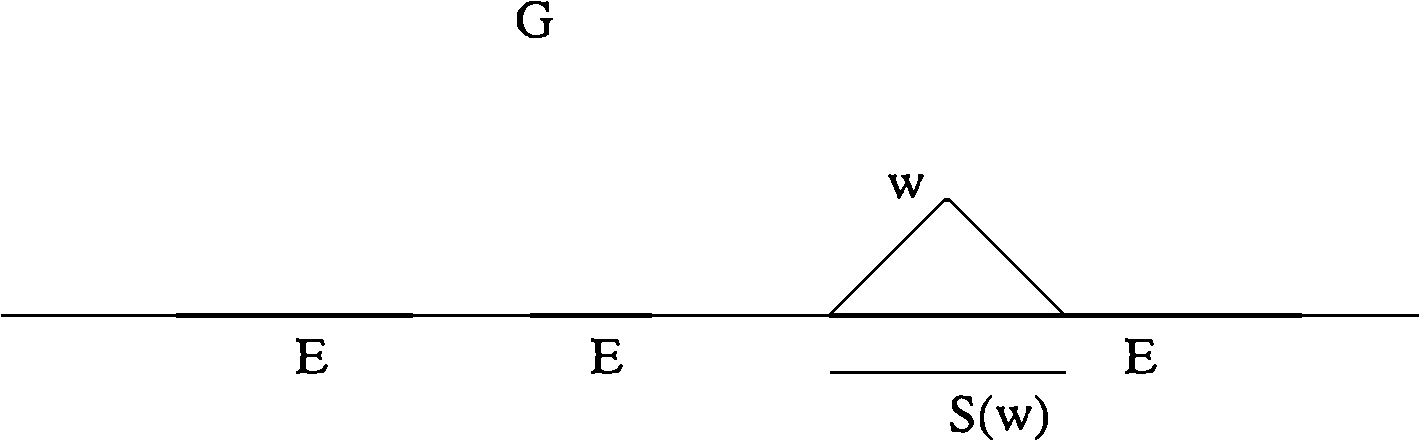
\includegraphics{Images/Img9.png}
    \bigskip
    \caption{Diagram for Proposition \ref{prop:ch4_6.3}.}
    \label{fig:ch4_6.1}
\end{figure}

Let $G = \cup_{z\in E^c}C(z)$. If $w \in G^c$, then $S(w) \subseteq E$, so $\P^w(X_\tau \in E) > c$. Hence
\begin{align*}
    \P^{(0,s)}(X_\tau \in E) &\geq \P^{(0,s)}(X_\tau \in E, \tau_G < \tau) \\
    &= \E^{(0,s)}[\P^{X_{\tau_G}}(X_\tau \in E); \tau_G < \tau] \\
    &\geq c\P^{(0,s)}(\tau_G < \tau).
\end{align*}
If $U^* > \lambda$, then the path of $Z_t$ must enter $G^c$ before $\tau$. So
\[
    \P^{(0,s)}(\tau_G < \tau) \geq \P^{(0,s)}(U^* > \lambda).
\]
\end{proof}

\begin{proof}[Proof of Theorem \ref{thm:ch4_6.2}, (a) implies (b)]
From Proposition \ref{prop:ch4_6.3},
\[
    s^d\P^{(0,s)}(U^* > \lambda) \leq cs^d\P^{(0,s)}(X_\tau \in E) \leq |E| = |\{N(f) > \lambda\}|.
\]
Integrating over $\lambda$ from $0$ to $\infty$, $s^d\E^{(0,s)}U^* \leq \int N(f)(x)dx$. Now let $s \to \infty$.
\end{proof}

We need the following lemmas. Suppose $v$ is a nonnegative function on $D$ and set $N_a(v)(x) = \sup_{z\in C_a(x)} v(z)$.

\begin{lemma}\label{lem:ch4_6.4}
If $b > a$,
\[
    |\{x : N_b(v)(x) > \lambda\}| \leq (1+(b/a)^d)|\{x : N_a(v)(x) > \lambda\}|.
\]
\end{lemma}

\begin{proof}
Let $f(t) = 1_{(N_a(v)>\lambda)}(t)$. If $N_b(v)(w) > \lambda$, there exists $(x,y)$ such that $|w-x| < by$ and $v(x,y) > \lambda$. So for any $t \in \R^d$ with $|t-x| < ay$, $N_a(v)(t) > \lambda$, or $f(t) = 1$. Hence $f = 1$ on $B(x,ay)$.

$B(x,ay) \subseteq B(w,ay+by)$, hence
\begin{align*}
    Mf(x) &\geq \frac{1}{|B(x,ay+by)|} \int_{B(w,ay+by)} f(t)dt \\
    &\geq \frac{|B(x,ay)|}{|B(w,ay+by)|} = \frac{a^d}{(a+b)^d}.
\end{align*}
So if $N_b(v)(w) > \lambda$, $Mf(w) \geq \alpha = a^d/(a+b)^d$. Then
\[
    |\{N_b(v) > \lambda\}| \leq |\{Mf \geq \alpha\}| \leq \frac{c}{\alpha}\|f\|_1 = \frac{c}{\alpha}|\{N_a(v) > \lambda\}|.
\]
\end{proof}

\begin{corollary}\label{cor:ch4_6.5}
If $b > a$,
\[
    \|N_b^h(f)\|_1 \leq (1+(b/a)^d)\|N_a^h(f)\|_1.
\]
\end{corollary}

[$N_b^h(f)$ is defined in \eqref{eq:ch4_6.1}.]

\begin{proof}
Applying Lemma \ref{lem:ch4_6.4} to $v(x,y) = u(x,y)1_{(y<h)}$, we see that
\begin{equation}\label{eq:ch4_6.2}
|\{N_b^h(f) > \lambda\}| \leq (1+(b/a)^d)|\{N_a^h(f) > \lambda\}|.
\end{equation}
Integrating \eqref{eq:ch4_6.2} over $\lambda$ from $0$ to $\infty$ proves the corollary.
\end{proof}

\begin{lemma}\label{lem:ch4_6.6}
There exist $a_0$ and $c$ depending only on the dimension such that if $a \leq a_0$, then
\[
    \|N_a^{2h}(f)\|_1 \leq \|N_a^h(f)\|_1 + c\limsup s^d\E^{(0,s)}U^*.
\]
\end{lemma}

\begin{proof}
We have $s^d\E^{(0,s)}|f(X_\tau)| \leq s^d\E^{(0,s)}U^*$, and letting $s \to \infty$,
\begin{equation}\label{eq:ch4_6.3}
    \int |f(x)|dx \leq \limsup s^d\E^{(0,s)}U^*.
\end{equation}
It follows that
\begin{equation}\label{eq:ch4_6.4}
    \|P_y f\|_1 = \|P_y * f\|_1 \leq \|P_y\|_1\|f\|_1 \leq \|f\|_1
\end{equation}
or
\[
    \int |u(x,y)|dx \leq \|f\|_1
\]
for all $y$.

Let $v_h^*(w) = \sup\{|u(x,y)| : (x,y) \in C_a(w), h \leq y < 2h\}$. Fix $w$. Provided $a_0$ is chosen small enough, if $(x,y) \in C_a(w)$ with $h \leq y < 2h$, then $B((x,y),h/2) \subseteq B(w,3h/2) \times [h/4,11h/4]$. Since $u$ is harmonic,
\begin{align*}
    |u(x,y)| &= ch^{-(d+1)}\Big|\int_{B((x,y),h/2)} u(z)dz\Big| \\
    &\leq ch^{-d-1}\int_{B(w,3h/2)}\int_{h/4}^{11h/4} |u(t,r)|dr\,dt.
\end{align*}
Integrating over $w \in \R^d$ and using Fubini's theorem,
\begin{align}\label{eq:ch4_6.5}
    \int v_h^*&(w)dw \\
    &\leq ch^{-d-1}\int\int_{B(w,3h/2)}\int_{h/4}^{11h/4} |u(t,r)|dr\,dt\,dw \notag \\
    &\leq ch^{-1}\int_{h/4}^{11h/4}\int |u(t,r)|dt\,dr \notag \\
    &\leq c\limsup s^d\E^{(0,s)}U^*. \notag
\end{align}

To finish,
\begin{align*}
    |\{N_a^{2h}(f) > \lambda\}| &\leq |\{N_a^{2h}(f) > \lambda, N_a^h(f) \leq \lambda\}| + |\{N_a^h(f) > \lambda\}| \\
    &\leq |\{u_h^* > \lambda\}| + |\{N_a^h(f) > \lambda\}|.
\end{align*}
Integrating over $\lambda$ from $0$ to $\infty$ gives
\[
    \|N_a^{2h}(f)\|_1 \leq \|u_h^*\|_1 + \|N_a^h(f)\|_1.
\]
Now apply \eqref{eq:ch4_6.5}.
\end{proof}

Very similar is the following Lemma, whose proof is Exercise \ref{ex:ch4_26}.

\begin{lemma}\label{lem:ch4_6.7}
Let $\epsilon > 0$. There exist $a_0$ and $c$ depending only on the dimension $d$ such that if $a \leq a_0$,
\[
    \|N_a^{\epsilon/2}(P_{\epsilon}f)\|_1 \leq c\limsup s^d\E^{(0,s)}U^*.
\]
\end{lemma}

\begin{proof}[Proof of Theorem \ref{thm:ch4_6.2}, (b) implies (a)]
Note $C(w) + (0,\epsilon) \subseteq C(w)$. Let $S_\epsilon = \inf\{t : Y_t < \epsilon\}$. By the translation invariance of the Poisson kernel and of Brownian motion, $\sup_{(x,y)\in C(w)+(0,\epsilon)} |u(x,y)| \uparrow N(f)(w)$ as $\epsilon \to 0$ and $\limsup s^d\E^{(0,s)}\sup_{r\leq S_\epsilon} |U_r| \leq \limsup s^d\E^{(0,s)}U^*$ for $\epsilon > 0$. Therefore it suffices to prove
\[
    \|N_a(f_\epsilon)\|_1 \leq c\limsup s^d\E^{(0,s)}U^*
\]
with $c$ independent of $\epsilon$, where $f_\epsilon = P_\epsilon f$, and then to let $\epsilon \to 0$.

Take $b_0 = 2a_0$ and let $K = 2(1+2^d)$. Let
\[
    E(\lambda,h) = \{x : N_{a_0}^h(f_\epsilon)(x) > \lambda, N_{b_0}^{2h}(f_\epsilon)(x) \leq K\lambda\}.
\]
We write
\begin{equation}\label{eq:ch4_6.6}
    |\{N_{a_0}^h(f_\epsilon) > \lambda\}| \leq |E(\lambda,h)| + |\{N_{b_0}^{2h}(f_\epsilon)/K > \lambda\}|.
\end{equation}

We will show there exists $c$ independent of $h$ and $\epsilon$ such that
\begin{equation}\label{eq:ch4_6.7}
    \int_0^\infty |E(\lambda,h)|\,d\lambda \leq c\limsup s^d\E^{(0,s)}U^*.
\end{equation}
Suppose we have \eqref{eq:ch4_6.7}. Integrating \eqref{eq:ch4_6.6} over $\lambda$ from $0$ to $\infty$, we have
\begin{align*}
    \|N_{a_0}^h(f_\epsilon)\|_1 &\leq \int_0^\infty |E(\lambda,h)|\,d\lambda + \|N_{b_0}^{2h}(f_\epsilon)/K\|_1 \\
    &\leq c\limsup s^d\E^{(0,s)}U^* + K^{-1}\|N_{b_0}^{2h}(f_\epsilon)\|_1 \\
    &\leq c\limsup s^d\E^{(0,s)}U^* + K^{-1}\|N_{a_0}^h(f_\epsilon)\|_1.
\end{align*}
Combining Lemma \ref{lem:ch4_6.7} and repeated uses of Lemma \ref{lem:ch4_6.6}, $\|N_{a_0}^h(f_\epsilon)\|_1 < \infty$. Using Corollary \ref{cor:ch4_6.5} we see that
\[
    \|N_{a_0}^h(f_\epsilon)\|_1 \leq 2c\limsup s^d\E^{(0,s)}U^*.
\]
Using Corollary \ref{cor:ch4_6.5} again, for any $a > 0$,
\[
    \|N_a^h(f_\epsilon)\|_1 \leq c\limsup s^d\E^{(0,s)}U^*.
\]
Letting $h \to \infty$ and then $\epsilon \to 0$ completes the proof.

It remains to prove \eqref{eq:ch4_6.7}. Let $R > 2h > 0$. Suppose $w \in E(\lambda,h)$. There exists $z = (x,y) \in C_{a_0}(w)$ with $y < h$ and $|u(x,y)| > \lambda$. Moreover there exists $c_1$ such that $|u| \leq K\lambda$ in $B(z,c_1y)$. By Corollary \chapref[II]{cor:ch4_1.4}, $|\nabla u| \leq c_2K\lambda/y$ in $B(z,c_1y/2)$. Hence there exists $c_3$ such that $|u| \geq \lambda/2$ in $B(z,c_3y)$. As in \eqref{eq:ch4_1.9}, since $|w| \leq 2R$, if $s$ is sufficiently large
\[
    \P_w^{(0,s)}(Z_t~\text{hits}~B(z,c_3y)~\text{before}~ \tau) \geq c.
\]
If $Z_t$ hits $B(z,c_3y)$ before $\tau$, $U^* \geq \lambda/2$.

Hence
\begin{align*}
    s^d\P^{(0,s)}(U^* &> \lambda/2) \\
    &\geq \int_{E(\lambda,h)\cap B(0,2R)} s^d\P_w^{(0,s)}(U^* > \lambda/2)\P^{(0,s)}(X_\tau \in dw) \\
    &\geq c\int_{E(\lambda,h)\cap B(0,2R)} s^d\P^{(0,s)}(X_\tau \in dw).
\end{align*}
For $s$ sufficiently large, this is greater than
\[
    c|E(\lambda,h) \cap B(0,2R)|.
\]
Integrate $\lambda$ from $0$ to $\infty$ to get
\[
    s^d\E^{(0,s)}U^* \geq c\int |E(\lambda,h) \cap B(0,2R)|\,d\lambda.
\]
Let $s \to \infty$ to show
\[
    \limsup s^d\E^{(0,s)}U^* \geq c\int |E(\lambda,h) \cap B(0,2R)|\,d\lambda.
\]
Letting $R \to \infty$, we then have \eqref{eq:ch4_6.7}.
\end{proof}

Recall that $u_j$ is the harmonic extension of $R_j f$. Let $u_0 = u$, write $\partial_0$ for $\partial_y$, and let $m_{ij} = \partial_i u_j$, $i,j = 0,1,\ldots,d$. Then
\[
    \widehat{m}_{ij}(\xi) = \im\xi^i \frac{\xi^j}{|\xi|}e^{-y|\xi|}\widehat{f}(\xi) = \widehat{m}_{ji}(\xi)
\]
if $i,j = 1,2,\ldots,d$, and a similar argument in the case when $i$ or $j$ is $0$ shows $m_{ij}$ is symmetric. Also
\[
    \trace \widehat{m}(\xi) = \widehat{m}_{00}(\xi)+\sum_{i=1}^d \widehat{m}_{ii}(\xi) = |\xi|e^{-y|\xi|}\widehat{f}(\xi)+\sum_{i=1}^d \frac{-(\xi^i)^2}{|\xi|}e^{-y|\xi|}\widehat{f}(\xi) = 0,
    % Note: changed \xi^j to \xi^i
\]
so the trace of $m$ is $0$.

\begin{proposition}\label{prop:ch4_6.8}
If $x \in \R^{d+1}$,
\begin{equation}\label{eq:ch4_6.8}
    \sum_i\Big(\sum_j m_{ij}x^j\Big)^2 \leq \frac{d}{d+1}\Big(\sum_{i,j} m_{ij}^2\Big)\sum_k(x^k)^2.
\end{equation}
\end{proposition}

\mpagebreak

\begin{proof}
Without loss of generality assume $\|x\|_2^2 = \sum_k(x^k)^2 = 1$. First suppose the matrix $m$ is diagonal with diagonal entries $\lambda_0,\ldots,\lambda_d$ and that $\lambda_{j_0}$ is the largest in absolute value. Since the trace of $m$ is $0$,
\[
    \lambda_{j_0} = -\sum_{j\neq j_0} \lambda_j,
\]
or by the Cauchy-Schwarz inequality,
\[
    \lambda_{j_0}^2 \leq d\sum_{j\neq j_0} \lambda_j^2.
\]
Hence $(d+1)\lambda_{j_0}^2 \leq d\sum_j \lambda_j^2$.

Now the left-hand side of \eqref{eq:ch4_6.8} is just
\begin{equation}\label{eq:ch4_6.9}
    \|mx\|_{\ell^2}^2 \leq \lambda_{j_0}^2 \leq \frac{d}{d+1}\sum_j \lambda_j^2 = \frac{d}{d+1}\sum_{i,j} m_{ij}^2.
\end{equation}

If $m$ is not diagonal, there exists a unitary matrix $P$ such that $n = P^tmP$ is diagonal. By Exercise \ref{ex:ch4_27}, $\sum_{i,j} m_{ij}^2 = \sum_{i,j} n_{ij}^2$. By the same exercise,
\begin{equation}\label{eq:ch4_6.10}
    \sup_{\|x\|_{\ell^2}\leq 1} \sum_i\Big(\sum_j m_{ij}x^j\Big)^2 = \sup_{\|x\|_{\ell^2}\leq 1} \sum_i\Big(\sum_j n_{ij}x^j\Big)^2.
\end{equation}
This with \eqref{eq:ch4_6.9} completes the proof.
\end{proof}

Let $F_\epsilon = (\epsilon^2 + \sum_{j=0}^d u_j^2)^{1/2}$, so that $F_\epsilon > 0$.

\index{Subharmonicity lemma|(}

\begin{proposition}[Subharmonicity lemma]\label{prop:ch4_6.9}
If $q > (d-1)/d$, then $\Delta(F_\epsilon^q) \geq 0$.
\end{proposition}

\begin{proof}
Note
\[
    \partial_i(F_\epsilon^q) = \frac{q}{2}\Big(\epsilon^2 + \sum_j u_j^2\Big)^{q/2-1}\Big(\sum_j 2u_j\partial_i u_j\Big)
\]
and
\begin{align*}
    \partial_{ii}^2(F_\epsilon^q) &= \frac{q}{2}\Big(\frac{q}{2}-1\Big)F_\epsilon^{q-4}\Big(\sum_j 2u_j\partial_i u_j\Big)^2 \\
    &\qquad+ \frac{q}{2}F_\epsilon^{q-2}\sum_j \Big[2(\partial_i u_j)^2 + 2u_j\partial_{ii}^2 u_j\Big].
\end{align*}
Since $\Delta u_j = 0$, summing over $i$ gives
\begin{equation}\label{eq:ch4_6.11}
    \Delta(F_\epsilon^q) = qF_\epsilon^{q-4}\Big[(q-2)\sum_i\Big(\sum_j u_j\partial_i u_j\Big)^2 + F_\epsilon^2\sum_{i,j}(\partial_i u_j)^2\Big].
\end{equation}
If $q \geq 2$, this is trivially $\geq 0$. Suppose $(d-1)/d < q < 2$. Let $m_{ij} = \partial_i u_j$, $x^j = u_j$. Then
\begin{align*}
    \sum_i\Big(\sum_j u_j\partial_i u_j\Big)^2 &= \sum_i\Big(\sum_j m_{ij}x^j\Big)^2 \\
    &\leq \frac{d}{d+1}\sum_{i,j}(\partial_i u_j)^2\sum_j u_j^2 \\
    &\leq \frac{d}{d+1}\sum_{i,j}(\partial_i u_j)^2 F_\epsilon^2.
\end{align*}
Hence the term inside the brackets in \eqref{eq:ch4_6.11} is greater than
\[
    (q-2)\frac{d}{d+1}F_\epsilon^2\sum_{i,j}(\partial_i u_j)^2 + F_\epsilon^2\sum_{i,j}(\partial_i u_j)^2.
\]
Since $q > (d-1)/d$, then $1+(q-2)d/(d+1) \geq 0$ and the last expression is greater than or equal to $0$.
\end{proof}

\index{Subharmonicity lemma|)}

We can now complete the proof of Theorem \ref{thm:ch4_6.2}.

\begin{proof}[Proof of Theorem \ref{thm:ch4_6.2}]
The equivalence of (a) and (b) was proved above. We show (d) implies (b). Let $(d-1)/d < q < 1$. Let $G_\epsilon = F_\epsilon^q$. Since $\Delta G_\epsilon \geq 0$, It\^o's formula tells us that
\[
    G_\epsilon(Z_{t\wedge\tau}) - G_\epsilon(Z_0) = \text{martingale} + \frac{1}{2}\int_0^{t\wedge\tau} \Delta G_\epsilon(Z_s)ds,
\]
or $G_\epsilon(Z_{t\wedge\tau})$ is a submartingale. $1/q > 1$, so by Doob's inequality,
\begin{align}\label{eq:ch4_6.12}
    \E^{(0,s)}\sup_{t<\tau} F_\epsilon(Z_t) &= \E^{(0,s)}\sup_{t<\tau} G_\epsilon(Z_t)^{1/q} \\
    &\leq c\E^{(0,s)}G_\epsilon(Z_\tau)^{1/q} = c\E^{(0,s)}F_\epsilon(Z_\tau). \notag
\end{align}
Let $\epsilon \to 0$. Then
\begin{align*}
    s^d\E^{(0,s)}U^* &\leq s^d\E^{(0,s)}\sup_{t<\tau} F(Z_t) \leq cs^d\E^{(0,s)}F(Z_\tau) \\
    &\leq c\sup_{y>0}\int |F(x,y)|dx.
\end{align*}

Next we show (d) implies (c). Just as above,
\[
    s^d\E^{(0,s)}\sup_{t<\tau} F(Z_t) \leq c\sup_{y>0}\int |F(x,y)|dx.
\]
However, $U_\tau^j \leq F(Z_\tau)$, so
\[
    \int |R_j f(x)|dx = \limsup cs^d\E^{(0,s)}U_\tau^j \leq c\sup_{y>0}\int |F(x,y)|dx.
\]
\mnewpage
This is true for $j = 1,2,\ldots,d$, and if we write $R_0$ for the identity, it is also true for $j = 0$.

To see that (b) implies (c) we use an argument very similar to the second proof of Theorem \ref{thm:ch4_3.5}. Let $g \in C_K^1$ with $\|g\|_\infty \leq 1$. Since $f \in H^1 \subseteq L^1$, arguing as in the first proof of Theorem \ref{thm:ch4_3.5} we obtain
\begin{align*}
    \int (R_j f)g &= \lim s^d\E^{(0,s)}\Big[g(X_\tau)\int_0^\tau \partial_y u_j(Z_r)dY_r\Big] \\
    &\leq \|g\|_\infty \limsup s^d\E^{(0,s)}\Big|\int_0^\tau A\nabla u(Z_r)\cdot dZ_r\Big|.
\end{align*}
By Theorem \chapref[I]{thm:ch1_6.8}, this is bounded by
\begin{align*}
    c\limsup \,&s^d\E^{(0,s)}\Big[\Big(\int_0^\tau |\nabla u(Z_r)|^2dr\Big)^{1/2}\Big] \\
    &\leq c\limsup s^d\E^{(0,s)}U^* + c\limsup s^d|u((0,s))| \\
    &\leq c\limsup s^d\E^{(0,s)}U^* + c\|f\|_1.
\end{align*}
Taking the supremum over such $gs$, we see
\begin{equation}\label{eq:ch4_6.13}
    \|R_j f\|_1 \leq c\limsup s^d\E^{(0,s)}U^* + c\|f\|_1.
\end{equation}
Since $|f(x)| \leq N(f)(x)$, by the equivalence of (a) and (b)
\[
    \|f\|_1 \leq \|N(f)\|_1 = \|f\|_{H^1} \leq \limsup s^d\E^{(0,s)}U^*.
\]
This and \eqref{eq:ch4_6.13} imply (c).

Finally, we want to see that (c) implies (d). Let $F_y(x,z) = F(x,y+z)$. So $F_y = P_yF$. We have
\begin{align*}
    \int |F(x,y)|dx &= \int F_y(x,0)dx \\
    &= \lim s^d\E^{(0,s)}F_y(Z_\tau) \\
    &\leq c\sum_{j=0}^d \lim s^d\E^{(0,s)}|P_yR_j f(Z_\tau)| \\
    &\leq c\sum \|P_yR_j f\|_1 \leq c\sum \|R_j f\|_1.
\end{align*}
\end{proof}

As an immediate corollary we have the following.

\begin{theorem}\label{thm:ch4_6.10}
If $f \in H^1$, then $f$ has nontangential limits\index{Nontangential limit} almost everywhere.
\end{theorem}

\begin{proof}
$f \in H^1$ implies that the harmonic extension of $f$, namely $u$, is such that $N(f) \in L^1$. Hence $u$ is nontangentially bounded a.e. The result follows by Theorem \ref{thm:ch4_1.5}.
\end{proof}

\mpagebreak

In the case $d=1$ we prove the boundedness of the Hilbert transform\index{Hilbert transform} on $H^1$.

\begin{proposition}\label{prop:ch4_6.11}
If $d = 1$, the Hilbert transform is bounded on $H^1$.
\end{proposition}

\begin{proof}
If $f \in H^1$, then $\limsup s^d\E^{(0,s)}U^* \leq c\|f\|_{H^1}$ by Theorem \ref{thm:ch4_6.2}. By Theorem \chapref[I]{thm:ch1_6.8},
\begin{align*}
    \limsup s^d\E^{(0,s)}(U_\tau)_\tau^{1/2} &\leq c\|f\|_{H^1} + \limsup s^d|u(0,s)| \\
    &\leq c\|f\|_{H^1} + c\|f\|_1 \leq c\|f\|_{H^1}.
\end{align*}
If $v$ is the harmonic extension of $Hf$ and $V_t = v(Z_{t\wedge\tau})$, then $(V)_\tau = (U)_\tau$. Using the inequalities of Theorem \chapref[I]{thm:ch1_6.8} again,
\begin{align*}
    \limsup s^d\E^{(0,s)}V^* &\leq c\|f\|_{H^1} + c\limsup s^d|v(0,s)| \\
    &\leq c\|f\|_{H^1} + \|Hf\|_1 \leq c\|f\|_{H^1}
\end{align*}
by Theorem \ref{thm:ch4_6.2}. Finally, again by Theorem \ref{thm:ch4_6.2}, $Hf \in H^1$ and $\|Hf\|_{H^1} \leq c\|f\|_{H^1}$.
\end{proof}

\subsecbkm{ch4_sec6.3}{Extensions}

Let us define $H^p$\index{H2@$H^p$} as follows.

\begin{definition}\label{def:ch4_6.12}
If $p \in (0,\infty)$, then $f$ is in $H^p$ if $N(f) \in L^p$ and we define $\|f\|_{H^p} = \|N(f)\|_p$.
\end{definition}

If $p > 1$, by Corollary \ref{cor:ch4_1.4} the $H^p$ norm of $f$ and the $L^p$ norm of $f$ are comparable. Note that for $p < 1$, $H^p$ is no longer a Banach space because the triangle inequality fails to hold.

Much of the $H^1$ theory goes through for $H^p$, $p < 1$. For example, the equivalence of (a) and (b) in Theorem \ref{thm:ch4_6.2} still holds if we replace $H^1$ by $H^p$ and $\lim s^d\E^{(0,s)}U^*$ by $\lim s^d\E^{(0,s)}(U^*)^p$. The equivalence of the analogs of (a) and (b) with (c) and (d) of Theorem \ref{thm:ch4_6.2} also continues to hold provided $p > (d-1)/d$. A suitable variation holds when $p \leq (d-1)/d$.

In Theorem \ref{thm:ch4_4.1} and Proposition \ref{prop:ch4_4.5} we saw that the area function\index{Area functional} was equivalent in $L^p$ norm to $f$ when $p > 1$. An examination of the proof of Proposition \ref{prop:ch4_4.5} shows that we actually proved that the $L^p$ norm of the area function of $f$ was bounded by a constant times the $H^p$ norm of $f$ for all $p$. It turns out that the inequality goes the other way as well. In fact, for all $p$, the $H^p$ norm of $f$ is equivalent to the $L^p$ norm of $A(f)$, the $L^p$ norm of $g(f)$, and the $L^p$ norm of $u^+$, where $u^+(x) = \sup_{y>0}|u(x,y)|$; see \cite{FeffermanStein1972} for the proofs.

Results for $H^p$ spaces can also be obtained through the use of atoms\index{Atoms}. For $H^1$ an atom is a function $a(x)$ having support in a cube $Q$ that is either bounded by $|Q|^{-1}$ and $\int a(x)=0$. It turns out that if $f$ is in $H^1$, then there exist constants $b_i$ and atoms $a_i$ such that $f(x)=\sum_i b_i a_i(x)$ and the $H_1$ norm of $f$ is comparable to $\sum|b_i|$ (see \cite{Coifman1974} and \cite{Latter1978}).

\section{Bounded mean oscillation}\label{ch4_sec7}

\subsecbkm{ch4_sec7.1}{Introduction}

The space $BMO$\index{BMO1@$BMO$} or space of functions of bounded mean oscillation is the
appropriate substitute for $L^\infty$ in many results concerning singular integrals. In this section we will consider the space $\BMO$\index{BMO2@$\BMO$} of martingales, the  relationship between $BMO$ and $\BMO$, prove that the dual of $H^1$ is $BMO$, and use $BMO$ to prove some strong results on the $L^p$ boundedness of singular integrals.

Let us start with the space $\BMO$ of martingales.

\begin{definition}\label{def:ch4_7.1}
A continuous martingale $M$ is in $\BMO$ if there exists $c$ such that for all stopping times $T$
\[
    \E[(M_\infty - M_T)^2|\FC_T] \leq c^2, \qquad \textnormal{a.s.}
\]
The smallest such $c$ is the $\BMO$ norm of $M$.
\end{definition}

Note that adding a $\FC_0$ measurable random variable to $M$ does not affect the $\BMO$ norm of $M$.

If $M$ is a bounded martingale, then $M \in \BMO$. For a slightly less trivial example, let $M_t = X_{t\wedge 1}$, where $X_t$ is Brownian motion. Then
\begin{align*}
    \E[(M_\infty - M_T)^2|\FC_T] &= \E[(X_1 - X_{1\wedge T})^2\mid \FC_T] \\
    &\leq \E[\sup_{s\leq 1}(X_{T+s} - X_T)^2\mid \FC_T] \\
    &= \E^{X_T}[\sup_{s\leq 1}(X_s - X_0)^2] = \E^0[\sup_{s\leq 1}X_s^2] \\
    &\leq c\E^0X_1^2 = c < \infty.
\end{align*}

If in the definition of $\BMO$ we integrate over $A = (T < \infty)$, we see that
\begin{equation}\label{eq:ch4_7.1}
    \E[(M_\infty - M_T)^2; T < \infty] \leq \|M\|^2_{\BMO}\P(T < \infty).
\end{equation}

In particular, if $M_0 \equiv 0$ and we take $T \equiv 0$, then $\E M_\infty^2 \leq \|M\|^2_{\BMO}$, or the $\BMO$ martingales can be considered as a subset of the square integrable ones.

Since $M_t^2 - \lrang{M}_t$ is a martingale, then $M \in \BMO$ if and only if
\begin{equation}\label{eq:ch4_7.2}
    \E[\lrang{M}_\infty - \lrang{M}_T\mid \FC_T] \leq c^2.
\end{equation}

\begin{proposition}[John-Nirenberg\index{John-Nirenberg ineq.}]\label{prop:ch4_7.2}
There exist $\alpha > 0$ and $c > 0$ such that if $M \in \BMO$, then
\[
    \E e^{\alpha M^*/\|M\|_{\BMO}} < c.
\]
\end{proposition}

\begin{proof}
By looking at $M/\|M\|_{\BMO}$, we may assume that the $\BMO$ norm of $M$ is $1$. By Jensen's inequality,
\[
    \E[|M_\infty - M_T||\FC_T] \leq (\E[(M_\infty - M_T)^2|\FC_T])^{1/2} \leq 1.
\]
The result now follows by Theorem \chapref[I]{thm:ch1_6.11}.
\end{proof}

Let
\begin{align}\label{eq:ch4_7.3}
    \MC^p = \{M &: M~\text{is a continuous martingale}, \\
    &\qquad M_0 = 0, \E(M_\infty^*)^p < \infty\}. \notag
\end{align}
For a norm on $\MC^p$ we use
\[
    \|M\|_{\MC^p} = \E[(M_\infty^*)^p]^{1/p}.
\]
By Theorem \chapref[I]{thm:ch1_6.8}, $\MC^p$ also equals $\{M : M_0 \equiv 0, \E\lrang{M}^{p/2} < \infty\}$. When $p > 1$, Doob's inequality implies that $\MC^p = L^p(\P)$, and in fact $\MC^p$ is isomorphic to $L^p(\P)$.

\subsecbkm{ch4_sec7.2}{Duality for martingales}

We will obtain the fact that $BMO$ is the dual of $H^1$\index{Dual of $H^1$} as a consequence of the corresponding duality of $\MC^1$ and $\BMO$.

\begin{proposition}\label{prop:ch4_7.3}
If $\varphi$ is a continuous linear functional on $\MC^1$, then there exists $Y \in \BMO$ such that for all $X \in \MC^2$,
\[
    \varphi(X) = \E X_\infty Y_\infty.
\]
\end{proposition}

\begin{proof}
Let us assume $\|\varphi\| = 1$. Since $\MC^2 \subseteq \MC^1$, then $\varphi$ is a continuous linear functional on $\MC^2$. Since $\MC^2$ is isomorphic to $L^2(\P)$, the dual of $\MC^2$ is $\MC^2$ itself. Therefore there exists $Y \in \MC^2$ such that $\varphi(X) = \E X_\infty Y_\infty$ for $X \in \MC^2$. We need to show that $Y \in \BMO$.

If $T$ is a stopping time, let $X_t = Y_t - Y_{t\wedge T}$, and let $Z = \lrang{X}_\infty$. Note $X_t = \int_0^t 1_{[T,\infty)}(s)dY_s$, so
\[
    \lrang{X,Y}_\infty = \int_0^\infty 1_{[T,\infty)}(s)d\lrang{Y}_s = \lrang{Y}_\infty.
\]
Hence
\[
    \E Z = \E\lrang{X,Y}_\infty = \E[(Y)_\infty - (Y)_T].
\]
On the other hand,
\mpagebreak
\[
    \E Z = \E\lrang{X,Y}_\infty = \E X_\infty Y_\infty = \varphi(X) \leq \|X\|_{\MC^1} \leq c\E[Z^{1/2}].
\]

Since $Z = 0$ on $(T = \infty)$, by the Cauchy-Schwarz inequality,
\[
    \E[Z^{1/2}] \leq (\E Z)^{1/2}\P(T < \infty)^{1/2},
\]
or $\E Z \leq c\P(T < \infty)$. So
\[
    \E[\lrang{Y}_\infty - \lrang{Y}_T] = \E Z \leq c\P(T < \infty).
\]
This is equivalent to $\E[\lrang{Y}_\infty - \lrang{Y}_T\mid \FC_T] \leq c$, or $Y \in \BMO$.
\end{proof}

\begin{proposition}[Fefferman's inequality\index{Fefferman's inequality}]\label{prop:ch4_7.4}
There exists $c$ such that if $X \in \MC^1$ and $Y \in \BMO$, then
\[
    \E\lrang{X,Y}_\infty \leq c\|X\|_{\MC^1}\|Y\|_{\BMO}.
\]
\end{proposition}

\begin{proof}
By stopping at suitable stopping times, we may assume that $X$, $Y$, $\lrang{X}$, and $\lrang{Y}$ are all bounded.

If we write
\[
    1 = \lrang{X}_t^{-1/4}\lrang{X}_t^{1/4},
\]
then by the inequalities of Kunita and Watanabe (Exercise \chapref[I.8]{ex:ch1_24}) and the Cauchy-Schwarz inequality,
\begin{align}\label{eq:ch4_7.4}
    (\E\lrang{X,Y}_\infty)^2 &\leq \Big(\E\Big[\int_0^\infty |d\lrang{X,Y}_s|\Big]\Big)^2 \\
    &\leq \Big(\E\int_0^\infty \lrang{X}_t^{-1/2}d\lrang{X}_t\Big)\Big(\E\int_0^\infty \lrang{X}_t^{1/2}d\lrang{Y}_t\Big). \notag
\end{align}

The first factor on the right in \eqref{eq:ch4_7.4} is equal to
\[
    \E[2\lrang{X}_\infty^{1/2}] \leq 2c\|X\|_{\MC^1}.
\]
For the second factor, we integrate by parts (cf.\ Corollary \chapref[I]{cor:ch1_5.7}):
\begin{align*}
    \E\int_0^\infty \lrang{X}_t^{1/2}d\lrang{Y}_t &= \E\lrang{X}_\infty^{1/2}\lrang{Y}_\infty - \E\int_0^\infty \lrang{Y}_t d\lrang{X}_t^{1/2} \\
    &= \E\int_0^\infty [\lrang{Y}_\infty - \lrang{Y}_t] d\lrang{X}_t^{1/2} \\
    &= \E\int_0^\infty \E[\lrang{Y}_\infty - \lrang{Y}_t\mid \FC_t]d\lrang{X}_t^{1/2} \\
    &\leq \|Y\|^2_{\BMO}\E\lrang{X}_\infty^{1/2} \leq c\|Y\|^2_{\BMO}\|X\|_{\MC^1}.
    % Note: it seems that we need \E\lrang{X}_\infty here
\end{align*}
Substituting these bounds in \eqref{eq:ch4_7.4} proves the proposition.
\end{proof}

If we define $\varphi(X) = \E X_\infty Y_\infty$ for $X \in \MC^2$, this inequality says that we can extend $\varphi$ to a continuous linear functional on $\MC^1$.

\subsecbkm{ch4_sec7.3}{Bounded mean oscillation}

Now let us turn to the analytic counterparts.

\begin{definition}\label{def:ch4_7.5}
We say $f$ is in $BMO$\index{BMO1@$BMO$} if there exists $c$ such that
\[
    \sup_Q \frac{1}{|Q|}\int_Q |f - f_Q| \leq c,
\]
where the supremum is over cubes in $\R^d$ (intervals if $d = 1$) and $f_Q$ denotes $|Q|^{-1}\int_Q f dx$. The smallest such $c$ is the $BMO$ norm of $f$.
\end{definition}

The space $BMO$ is only defined up to additive constants; that is, $f$ and $f + c$ have the same $BMO$ norm. $f - f_Q$ is the oscillation of $f$ about its mean (over $Q$), and the mean oscillation, namely, $|Q|^{-1}\int_Q|f - f_Q|$, is supposed to be bounded, which gives rise to the name $BMO$.

We have the analytic version of the John-Nirenberg inequality.\index{John-Nirenberg ineq.|(}

\begin{proposition}\label{prop:ch4_7.6}
There exists $\alpha$ such that for each cube $Q_0$
\begin{equation}\label{eq:ch4_7.5}
    \Big|\Big\{x \in Q_0 : \frac{|f - f_{Q_0}|}{\|f\|_{BMO}} > \lambda\Big\}\Big| \leq e^{-\alpha\lambda}.
\end{equation}
\end{proposition}

% Note: changed ||f||_{\BMO} to \|f\|_{BMO} in the next paragraph.

\begin{proof}
By scaling we may assume $Q_0$ is the unit cube and that $\|f\|_{BMO} = 1$. We consider $f$ as a dyadic martingale. Let $\FC_n$ be the $2^{nd}$ subcubes of $Q_0$ of side length $2^{-n}$ and set $f = X_n$. Then $f_Q = |Q|^{-1}\int_Q f$ is the value of $X_n$ for $\omega$ in the interior of $Q$, if $Q \in \FC_n$.

Our inequality will follow from Corollary \chapref[I]{cor:ch1_6.12} once we verify the hypotheses of that proposition. First of all, let $T$ be a stopping time. On the set $(T = n)$, if $Q$ is a cube in $\FC_n$ such that $\omega \in Q$, then
\[
    (X_\infty - X_T)(\omega) = f - f_Q.
\]
If $A \in \FC_\infty$, then $A \cap (T = n) \in \FC_n$, and so
\begin{align*}
    \E\big[|X_\infty - X_T|; A \cap (T = n)\big] &= \sum_{Q\in\FC_n,Q\subseteq A\cap(T=n)} \E\big[|X_\infty - X_T|; Q\big] \\
    &= \sum_{Q\in\FC_n,Q\subseteq A\cap(T=n)} \int_Q |f - f_Q| \\
    &\leq \|f\|_{BMO} \sum_{Q\in\FC_n,Q\subseteq A\cap(T=n)} |Q| \\
    &= \|f\|_{BMO}\P(A \cap (T = n)).
\end{align*}
It follows that $\E[|X_\infty - X_T|\mid \FC_T] \leq \|f\|_{BMO}$.

Secondly we must check that the jumps of $X_n$ are bounded. If $\omega \in Q \subseteq Q'$ with $Q \in \FC_{n+1}$, $Q' \in \FC_n$, then
\mpagebreak
\[
    (X_{n+1} - X_n)(\omega) = |Q|^{-1}\int_Q f - |Q'|^{-1}\int_{Q'} f = |Q|^{-1}\int_Q f - f_{Q'}.
\]
Therefore
\begin{align*}
    |(X_{n+1} - X_n)(\omega)| &\leq \frac{1}{|Q|}\int_Q |f - f_{Q'}| \\
    &\leq 2^d\frac{1}{|Q'|}\int_{Q'} |f - f_{Q'}| \leq 2^d\|f\|_{BMO}.
\end{align*}
We now apply Corollary \chapref[I]{cor:ch1_6.12}.
\end{proof}

\index{John-Nirenberg ineq.|)}

\begin{corollary}\label{cor:ch4_7.7}
\[
    \sup_Q \frac{1}{|Q|}\int |f - f_Q|^2 \leq c\|f\|^2_{BMO}.
\]
\end{corollary}

\begin{proof}
By scaling we may take $Q$ to be a unit cube. Multiply \eqref{eq:ch4_7.5} by $2\lambda$, integrate over $\lambda$ from $0$ to $\infty$ and use Proposition \chapref[I]{prop:ch1_1.5}.
\end{proof}

Let $u$ be the harmonic extension of $f$ and let $U_t = u(Z_{t\wedge\tau})$. One might guess that $f \in BMO$ if and only if $U_t \in \BMO$, and that turns out to be true.

\begin{proposition}\label{prop:ch4_7.8}
If $U_t \in \BMO$, then $f \in BMO$ and $\|f\|_{BMO} \leq c\|U\|_{BMO}$.
\end{proposition}

\begin{proof}
For any $t$, by the strong Markov property
\begin{equation}\label{eq:ch4_7.6}
    \|U\|^2_{\BMO} \geq \E[(U_\infty - U_t)^2\mid \FC_t] = \E^{Z_{t\wedge\tau}}[(U_\infty - U_0)^2].
\end{equation}
Let us write $P_Hf(z) = P_Hf(x,y)$ for $P_yf(x)$ if $z = (x,y)$. Under $\P^z$ we have $U_0 = u(z)$ while $U_\infty = f(X_\tau)$ and $\E^zU_\infty = \E^zf(X_\tau) = u(z)$. Thus
\begin{align*}
    \E^z[(U_\infty - U_0)^2] &= \E^z U_\infty^2 -2u(z)\E^z U_\infty + u(z)^2 \\
    &= \E^z[(f(X_\tau))^2] - u(z)^2.
\end{align*}
Therefore \eqref{eq:ch4_7.6} says that
\begin{equation}\label{eq:ch4_7.7}
    P_H(f^2)(Z_{t\wedge\tau}) - (P_Hf(Z_{t\wedge\tau}))^2 \leq \|U\|^2_{\BMO}, \qquad \text{a.s.}
\end{equation}
for each $t$.

Since $P_H(f^2)$ and $P_Hf$ are harmonic, they are continuous in $D$. We must have that
\begin{equation}\label{eq:ch4_7.8}
    P_H([f - P_Hf(z)]^2)(z) = P_H(f^2)(z) - (P_Hf(z))^2 \leq \|U\|^2_{\BMO}
\end{equation}
for all $z \in D$. For if not, there is a neighborhood of $z$ in which the left-hand side of \eqref{eq:ch4_7.8} is strictly greater than the right-hand side. However, $Z_t$ will hit this neighborhood before leaving $D$ with positive probability, which contradicts \eqref{eq:ch4_7.7}.

We want to obtain a bound on $|Q|^{-1}\int_Q |f - f_Q|^2$. By scaling and translation, we may assume $Q$ is the unit cube in $\R^d$ centered at $0$. Let $z_0 = (0,\ldots,0,1)$. Note
\begin{align}\label{eq:ch4_7.9}
    |Q|^{-1}\int_Q (f-&P_Hf(z_0))^2 \\
    &= |Q|^{-1}\int_Q f^2 - 2f_QP_Hf(z_0) + (P_Hf(z_0))^2 \notag \\
    &= |Q|^{-1}\int_Q f^2 - f_Q^2 + (f_Q - P_Hf(z_0))^2 \notag \\
    &\geq |Q|^{-1}\int_Q f^2 - f_Q^2 \notag \\
    &= |Q|^{-1}\int_Q (f - f_Q)^2. \notag
\end{align}
Also, $|Q|^{-1}1_Q(y) \leq cP_H(z_0,y)$, so
\[
    |Q|^{-1}\int_Q (f - P_Hf(z_0))^2 \leq cP_H\big([f - P_Hf(z_0)]^2\big)(z_0).
\]
Combining this, \eqref{eq:ch4_7.8}, and \eqref{eq:ch4_7.9} shows
\[
    |Q|^{-1}\int_Q |f - f_Q|^2 \leq c\|U\|^2_{\BMO}.
\]
An application of Jensen's inequality finishes the proof.
\end{proof}

\begin{proposition}\label{prop:ch4_7.9}
If $f \in BMO$, then $U_t \in \BMO$ and $\|U\|_{\BMO} \leq c\|f\|_{BMO}$.
\end{proposition}

\begin{proof}
By the proof of Proposition \ref{prop:ch4_7.8},
\[
    \E[|U_\infty - U_T|^2\mid \FC_T] = P_H\big([f - P_Hf(Z_T)]^2\big)(Z_T).
\]
So we want to show $P_H\big([f - P_Hf(z)]^2\big)(z) \leq c\|f\|^2_{BMO}$ for each $z$. By scaling and translation, it is enough to show it for $z_0 = (0,\ldots,0,1)$.

Let $Q_0$ be the unit cube in $\R^d$ centered at $0$ and $Q_n = 2^nQ_0$. As in (7.9),
\begin{align*}
    P_H\big([f - f_{Q_0}]^2\big)(z_0) &= P_H\big([f - P_Hf(z_0)]^2\big)(z_0) + \big(P_Hf(z_0) - f_{Q_0}\big)^2 \\
    &\geq P_H\big([f - P_Hf(z_0)]^2\big)(z_0).
\end{align*}
Now $P_H(z_0,x) \leq c\sum_{n=0}^\infty 2^{-n}|Q_n|^{-1}1_{Q_n}(x)$. So
\mpagebreak
\begin{equation}\label{eq:ch4_7.10}
    P_H\big([f - P_Hf(z_0)]^2\big)(z_0) \leq c\sum 2^{-n}\frac{1}{|Q_n|}\int_{Q_n} |f - f_{Q_0}|^2.
\end{equation}
By the triangle inequality and the Cauchy-Schwarz inequality,
\[
    \frac{1}{|Q_n|}\int_{Q_n} |f - f_{Q_0}|^2 \leq \frac{n}{|Q_n|}\int_{Q_n} |f - f_{Q_n}|^2 + n\sum_{i=0}^{n-1}|f_{Q_{i+1}} - f_{Q_i}|^2.
\]
As in the proof of Proposition \ref{prop:ch4_7.6}, $|f_{Q_{i+1}} - f_{Q_i}| \leq c\|f\|_{BMO}$. So
\[
    \frac{1}{|Q_n|}\int_{Q_n} |f - f_{Q_0}|^2 \leq cn\|f\|^2_{BMO} + cn^2\|f\|^2_{BMO}.
\]
Substituting in \eqref{eq:ch4_7.10},
\[
    P_H\big([f - P_Hf(z_0)]^2\big)(z_0) \leq c\sum(1 + n^2)2^{-n}\|f\|^2_{BMO} \leq c\|f\|^2_{BMO}.
\]
\end{proof}

\subsecbkm{ch4_sec7.4}{The dual of \texorpdfstring{$H^1$}{H¹}}
\index{Dual of $H^1$|(}

We now prove the $H^1 - BMO$ duality in the analytic case. The first fact we need is that $R_j$ maps $L^\infty$ to $BMO$. Later, we will want a similar result for more general kernels, so we take care of both at once.

\begin{proposition}\label{prop:ch4_7.10}
Suppose $K : \R^d \to \R$ satisfies \eqref{eq:ch4_5.11} and there exists $c_1$ such that
\begin{equation}\label{eq:ch4_7.11}
    |K(x)| \leq c_1|x|^{-d}, \qquad x \neq 0
\end{equation}
and
\begin{equation}\label{eq:ch4_7.12}
    \|Kf\|_2 \leq c_1\|f\|_2.
\end{equation}
Then there exists $c_2$ such that if $f \in L^\infty$ with compact support, then $Kf \in BMO$ and $\|Kf\|_{BMO} \leq c_2\|f\|_\infty$.
\end{proposition}

By our results in Sect.\ \ref{ch4_sec3}, we see that the Riesz transforms $R_j$ satisfy the hypotheses of this proposition.

\begin{proof}
Let $Q$ be a cube and $Q'$ the cube with the same center but twice the side length. Let $f = f_1 + f_2$ where $f_1 = f1_{Q'}$. By scaling we may assume $|Q| = 1$ and that $Q$ is centered at the origin.
\begin{align*}
    \Big(\frac{1}{|Q|}\int_Q |Kf_1(x)|dx\Big)^2 &\leq \frac{1}{|Q|}\int_Q |Kf_1(x)|^2dx \leq \frac{1}{|Q|}\|Kf_1\|_2^2 \\
    &\leq \frac{1}{|Q|}c\|f_1\|_2^2 \leq \frac{c\|f\|_\infty^2}{|Q|}|Q'|^2.
\end{align*}

\mpagebreak

Let $a = \int K(-y)f_2(y)dy$. So
\begin{align*}
    |Kf_2(x) - a| &= \Big|\int[K(x-y) - K(-y)]f_2(y)dy\Big| \\
    &\leq \|f\|_\infty \int_{(Q')^c} |K(x-y) - K(-y)|dy \leq c\|f\|_\infty
\end{align*}
by \eqref{eq:ch4_5.11}. Then
\[
    \frac{1}{|Q|}\int_Q |Kf_2(x) - a| \leq c\|f\|_\infty.
\]
Combining
\[
    \frac{1}{|Q|}\int_Q |Kf(x) - a| \leq c\|f\|_\infty.
\]
Our result follows since
\begin{align*}
    |Q|^{-1}\int_Q |Kf - (Kf)_Q| &\leq |Q|^{-1}\int_Q |Kf - a| + |(Kf)_Q - a| \\
    &= 2|Q|^{-1}\int_Q |Kf - a| \leq c\|f\|_\infty.
\end{align*}
\end{proof}

To verify \eqref{eq:ch4_7.12} we have

\begin{proposition}\label{prop:ch4_7.11}
Suppose $K$ satisfies (7.11), (5.11) and
\begin{equation}\label{eq:ch4_7.13}
    \int_{R_1<|x|<R_2} K(x) = 0 \qquad \text{for all}~0 < R_1 < R_2.
\end{equation}
Then there exists $c$ such that $|\widehat{Kf}(\xi)| \leq c|\widehat{f}(\xi)|$ for all $f \in L^2$.
\end{proposition}

\begin{proof}
It suffices to show the inequality for $f \in C_K^\infty$. For such $f$ it is not hard to see (cf.\ Proposition \ref{prop:ch4_2.3}) that $\lim_{\epsilon\to 0,N\to\infty}\widehat{K_{\epsilon N}f}(\xi) \to \widehat{Kf}(\xi)$, where $K_{\epsilon N}(x) = K(x)1_{\epsilon<|x|<N}$, and so we need only look at $\widehat{K_{\epsilon N}f}(\xi) = \widehat{K_{\epsilon N}}(\xi)\widehat{f}(\xi)$.

Fix $\xi$. If $\epsilon$ is small enough and $N$ is large enough,
\begin{equation}\label{eq:ch4_7.14}
    \widehat{K_{\epsilon N}}(\xi) = \int_{\epsilon<|x|<N} e^{\im\xi\cdot x}K(x)dx = \int_{\epsilon<|x|\leq 10/|\xi|} + \int_{10/|\xi|<|x|<N}
\end{equation}
Since $K$ satisfies \eqref{eq:ch4_7.11} and \eqref{eq:ch4_7.13},
\begin{align}\label{eq:ch4_7.15}
    \int_{\epsilon<|x|\leq 10/|\xi|} e^{\im\xi\cdot x}K(x)dx &= \int_{\epsilon<|x|\leq 10/|\xi|} [e^{\im\xi\cdot x} - 1]K(x)dx \\
    &\leq \int_{|x|\leq 10/|\xi|} \frac{c}{|x|^d}|\xi\cdot x|dx \leq c. \notag
\end{align}

\mpagebreak

To handle the second integral in \eqref{eq:ch4_7.14}, let $z = \pi\xi/|\xi|^2$ so that $e^{\im z\cdot\xi} = -1$ and $|z| = \pi/|\xi|$.
\begin{equation}\label{eq:ch4_7.16}
    \int K_{\epsilon N}(x)e^{\im\xi\cdot x}dx = -\int K_{\epsilon N}(x-z)e^{\im\xi\cdot x}dx
\end{equation}
by a change of variables. So
\[
    \int K_{\epsilon N}(x)e^{\im\xi\cdot x}dx = \frac{1}{2}\int[K_{\epsilon N}(x) - K_{\epsilon N}(x-z)]e^{\im\xi\cdot x}dx
\]
and
\begin{align}\label{eq:ch4_7.17}
    \int_{10/|\xi|<|x|} &K_{\epsilon N}(x)e^{i\xi\cdot x}dx \\
    &= \frac{1}{2}\int_{10/|\xi|<|x|}[K_{\epsilon N}(x) - K_{\epsilon N}(x-z)]e^{\im\xi\cdot x}dx \notag \\
    &\qquad-\int_{|x|\leq 10/|\xi|} K_{\epsilon N}(x)e^{\im\xi\cdot x}dx \notag \\
    &\qquad+\frac{1}{2}\int_{|x|\leq 10/|\xi|}[K_{\epsilon N}(x) - K_{\epsilon N}(x-z)]e^{\im\xi\cdot x}dx. \notag
\end{align}

The second integral on the right in \eqref{eq:ch4_7.17} we have already handled. Note $1/|\xi| = |z|/\pi$. If $|x| \geq 10|z|/\pi$, the only way for $|x|$ to be larger than $N$ and $|x-z|$ less than $N$ or vice versa is if $N/10 \leq |x| \leq 10N$. So the first integral on the right in \eqref{eq:ch4_7.17} is bounded, using \eqref{eq:ch4_5.11} and \eqref{eq:ch4_7.11}, by
\begin{align*}
    \int_{|x|\geq 10|z|/\pi} |K_{\epsilon N}(x)- &K_{\epsilon N}(x-z)|dx \\
    &\leq \int_{|x|\geq 10|z|/\pi} |K(x) - K(x-z)|dx \\
    &\qquad +2\int_{N/10\leq|x|\leq 10N} |K(x)|dx \leq c.
\end{align*}
For the third integral on the right in \eqref{eq:ch4_7.17}, because of \eqref{eq:ch4_7.15} we need to consider only
\begin{align}\label{eq:ch4_7.18}
    \int_{|x|\leq 10/|\xi|} &K_{\epsilon N}(x-z)e^{\im\xi\cdot x}dx \\
    &= -\int_{|x+z|\leq 10/|\xi|} K_{\epsilon N}(x)e^{\im\xi\cdot x}dx \notag \\
    &= -\int_{\epsilon<|x|<1/|\xi|} K(x)e^{\im\xi\cdot x}dx \notag \\
    &\qquad-\int_{1/|\xi|<|x|,|x+z|\leq 10/|\xi|} K(x)e^{\im\xi\cdot x}dx. \notag
\end{align}
The first integral on the right in \eqref{eq:ch4_7.18} is similar to what we did in \eqref{eq:ch4_7.15} and
\[
    \Big|\int_{1/|\xi|<|x|,|x+z|\leq 10/|\xi|}K(x)e^{\im\xi\cdot x}\Big|\le c\int_{1/|\xi|\leq |x| \leq 15/|xi|}|x|^{-d}dx\le c.
\]
\end{proof}

We now show that every $BMO$ function gives rise to a similar functional on $H^1$.

\begin{proposition}\label{prop:ch4_7.12}
If $g \in BMO$ and $\varphi(f) = \int fg$ for $f \in C_K^\infty$, then $\varphi$ has a bounded extension to $H^1$ with $\|\varphi\| \leq c\|g\|_{BMO}$.
\end{proposition}

\begin{proof}
Let $u$ and $v$ be the harmonic extensions of $f$ and $g$, respectively, and let $U_t = u(Z_{t\wedge\tau})$, $V_t = v(Z_{t\wedge\tau})$.
\begin{align*}
    \varphi(f) &= \lim s^d\E^{(0,s)}f(X_\tau)g(X_\tau) = \lim s^d\E^{(0,s)}U_\tau V_\tau \\
    &\leq (c\limsup s^d\E^{(0,s)}U_\tau^*)\|V\|_{BMO} \leq c\|f\|_{H^1}\|g\|_{BMO}.
\end{align*}
This completes the proof.
\end{proof}

As a consequence we have Fefferman's inequality\index{Fefferman's inequality} for functions:
\begin{equation}\label{eq:ch4_7.19}
    \Big|\int fg\Big| \leq c\|f\|_{H^1}\|g\|_{BMO}.
\end{equation}

We show that every linear functional on $H^1$ arises from a $BMO$ function. This is the content of Proposition \ref{prop:ch4_7.15}, but we need a few propositions first.

Let
\[
    H_0^1 = \{f \in H^1 : f~\text{is in the Schwartz class}\}.
\]

\begin{proposition}\label{prop:ch4_7.13}
$H_0^1$ is dense in $H^1$.
\end{proposition}

\begin{proof}
Let $A_1 = \{f \in H^1 : \widehat{f}$ has compact support not containing $0\}$ and $A_2 = \{f \in A_1 : \widehat{f} \in C^\infty\}$. We will show $A_1$ is dense in $H^1$ and $A_2$ is dense in $A_1$. That will prove the proposition, for if $f \in A_2$, then $\widehat{f}$ is in the Schwartz class, and hence so is $f$.

Let $\varphi$ be a $C^\infty$ radially symmetric function on $\R^d$ with compact support such that $\varphi(x) = 1$ if $|x| \leq 1$. Let $\Phi$ be the function such that $\widehat{\Phi} = \varphi$. Define $T_\delta$ by $\widehat{T_\delta f}(\xi) = \varphi(\xi/\delta)\widehat{f}(\xi)$. So
\[
    T_\delta f(x) = \delta^d \int f(x-y)\Phi(\delta y)dy.
\]
$\varphi$ is in the Schwartz class, hence so is $\Phi$. This implies that $\Phi$ is integrable, and hence by scaling there exists $c$ such that $\|T_\delta f\|_1 \leq c\|f\|_1$ for all $\delta$. Note that $\int \Phi(x)dx = \varphi(0) = 1$.

Let $f \in H^1$ and let $f_k = T_k(I - T_{1/k})f$. It is not hard to see that if $g \in C_K^\infty$, then $(I - T_{1/k})g \to g$ uniformly and then $T_k(I - T_{1/k})g \to g$ in $L^1$. By the uniform boundedness of the $T_\delta$ and the fact that $C_K^\infty$ is dense in $L^1$, we obtain that $f_k \to f$ in $L^1$. Since $f \in H^1$, then $R_jf \in L^1$. So $R_jf_k = T_k(I - T_{1/k})R_jf \to R_jf$ in $L^1$. Consequently $f_k \to f$ in $H^1$. Since $\widehat{f_k}(\xi) = \varphi(\xi/k)[\widehat{f}(\xi)-\varphi(k\xi)\widehat{f}(\xi)]$, $\widehat{f_k}$ has compact support disjoint from $0$, or $A_1$ is dense in $H^1$.

Next suppose $f \in A_1$. Let $\psi$ be in $C_K^\infty$ with $\int \psi(\xi)d\xi = 1$. Let $\Psi$ satisfy $\widehat{\Psi}=\psi$. Let $\psi_k(\xi)=k^d\psi(k\xi)$. Define $f_k$ by $\widehat{f_k}(\xi) = (\widehat{f} * \psi_k)(\xi)$. Then $\widehat{f_k}$ is $C^\infty$ with compact support, and there is a neighborhood $V$ of the origin such that for $k$ large enough, $\widehat{f_k}$ is $0$ in $V$. $\widehat{f_k}$ is the Fourier transform of $f_k(x) = f(x)\Psi(x/k)$. It is not hard to see that $f_k \to f$ in $L^1$. Let $M_j$ be a function such that $\widehat{M_j} = m_j = \im x^j/|x|$ outside of $V$ and $m_j \in C_K^\infty$. Then $M_j$ is in the Schwartz class and hence integrable. Since $f,f_k \in A_1$,
\[
    R_jf_k = M_j * f_k \to M_j * f = R_jf
\]
in $L^1$. Therefore $f_k \to f$ in $H^1$, and $A_2$ is dense in $A_1$.
\end{proof}

\begin{proposition}\label{prop:ch4_7.14}
Suppose $g \in L^\infty$. Then there exists $h$ with $\|h\|_{BMO} \leq c\|g\|_\infty$ such that
\[
    \int (R_jf)g = \int fh
\]
for all $f \in H^1$. $c$ does not depend on $g$.
\end{proposition}

The idea is that one would like to write $\int(R_jf)g = -\int f(R_jg)$, and by Proposition \ref{prop:ch4_7.10}, we should have $\|-R_jg\|_{BMO} \leq c\|g\|_\infty$. The difficulty is that $R_jg$ may not be defined when $g \in L^\infty$, and we have to go through some contortions to sidestep this.

\begin{proof}
Let
\[
    g_N(y) = g(y)1_{(|y|\leq N)},
\]
\[
    h_N(x) = -\int g_N(y)\big[K_j(x-y) - 1_{(|y|\geq 1)}K_j(-y)\big]dy,
\]
\[
    k_N(x) = -\int g_N(y)\big[K_j(x-y)1_{B(x,1)}(y)\big]dy,
\]
and
\[
    \ell_N(x) = -\int g_N(y)\big[K_j(x-y)1_{B(x,1)^c}(y) - 1_{(|y|\geq 1)}K_j(-y)\big]dy,
\]
where $K_j(z) = cz^j/|z|^{d+1}$ is the kernel for the $j$th Riesz transform.

Since $g_N \in L^p$ for all $p$, $R_jg_N(x)$ exists for almost every $x$. Since $g_N$ has compact support, it follows that $h_N$, $k_N$, and $\ell_N$ exist for almost every $x$. $h_N(x)$ differs from $-R_jg_N(x)$ by $\int_{|y|\geq 1} g_N(y)K_j(-y)dy$. This is a constant, and since $BMO$ is defined only up to additive constants,
\[
    \|h_N\|_{BMO} = \|R_jg_N\|_{BMO} \leq c\|g_N\|_\infty
\]
by Proposition \ref{prop:ch4_7.10}.

Let us show $h_N(x)$ converges for almost every $x$ as $N \to \infty$ and that the convergence is uniform on compacts. For $|x| \leq R$, $k_N(x) = -\int g(y)K_j(x-y)1_{B(x,1)}(y)dy$ for all $N \geq R + 1$, so the $k_N$s converge. Call the limit $k$. Provided $|x| \leq R$, $|y-x| \geq 1$, and $|y| \geq 1$,
\begin{equation}\label{eq:ch4_7.20}
|K_j(x-y) - K_j(-y)| \leq c|x|/|y|^{d+1}
\end{equation}
is absolutely integrable in $y$. So if $|x| \leq R$ and $N,M \geq R + 1$,
\begin{align}\label{eq:ch4_7.21}
    |\ell_N(x) - \ell_M(x)|& \\
    &\leq 2\|g\|_\infty \int_{|y|\geq N\wedge M} |K_j(x-y) - K_j(-y)|dy \notag \\
    &\leq \frac{c|x| \|g\|_\infty}{N \wedge M} \to 0 \notag
\end{align}
as $N,M \to \infty$. Let $\ell(x) = \lim_{N\to\infty} \ell_N(x)$. Since $h_N = k_N + \ell_N$, $h_N(x)$ converges, say to $h(x)$, uniformly on compacts.

If $Q$ is a cube, then
\[
    |Q|^{-1}\int_Q |h - h_Q| = \lim_N |Q|^{-1}\int_Q |h_N - (h_N)_Q| \leq c\|g\|_\infty,
\]
by virtue of the uniform convergence. So $\|h\|_{BMO} \leq c\|g\|_\infty$.

Because $f \in H^1$, $\int f(x)dx = 0$ (Exercise \ref{ex:ch4_24}).
\[
    \int (R_jf)g_N = -\int f(R_jg_N) = \int f(-R_jg_N - a_N)
\]
for any constant $a_N$. Taking $a_N = \int_{|y|\geq 1} g_N(y)K_j(-y)dy$,
\[
    \int (R_jf)g_N = \int fh_N.
\]
We must now let $N \to \infty$ and show we can pass to the limit. The left-hand side is easy. If $f \in H^1$, then $R_jf \in L^1$ and
\[
    \Big|\int (R_jf)g_N - \int (R_jf)g\Big| \leq \|g\|_\infty \int_{|y|\geq N} |R_jf(y)|dy \to 0
\]
as $N \to \infty$.

It remains to show convergence of the right-hand side. Since $H_0^1$ is dense in $H^1$, by \eqref{eq:ch4_7.19} it suffices to show
\mpagebreak
\begin{equation}\label{eq:ch4_7.22}
    \lim_{N\to\infty} \int fh_N = \int fh, \qquad f \in H_0^1.
\end{equation}
Let $f \in H_0^1$, let $\epsilon > 0$, and choose $R$ such that $\int_{|x|>R} |f(x)|^2|x|^{4d+4}dx < \epsilon^2$. Since $h_N \to h$ uniformly on $B(0,R)$, we concentrate on $B(0,R)^c$ and show
\begin{equation}\label{eq:ch4_7.23}
    \sup_N\Big|\int_{B(0,R)^c} fh_N\Big| \leq c\epsilon, \qquad \Big|\int_{B(0,R)^c} fh\Big| < c\epsilon.
\end{equation}

$L(y) = K_j(y)1_{(|y|\leq 1)}$ is a kernel to which Proposition \ref{prop:ch4_7.11} applies. $k_N(x) = -Lg_N(x)$, so
\begin{equation}\label{eq:ch4_7.24}
    \int |k_N|^2 \leq c\int |g_N|^2 \leq c\int_{B(0,N)} |g|^2 \leq cN^d.
\end{equation}
Hence if $N \leq M + 1$,
\begin{equation}\label{eq:ch4_7.25}
    \int_{B(0,M)} |k_N|^2 \leq cN^d \leq cM^d.
\end{equation}
If $|x| \leq M$ and $N > M + 1$, then $k_N(x) = k_{M+1}(x)$, so
\begin{equation}\label{eq:ch4_7.26}
    \int_{B(0,M)} |k_N|^2 = \int_{B(0,M)} |k_{M+1}|^2 \leq \int |k_{M+1}|^2 \leq cM^d
\end{equation}
by \eqref{eq:ch4_7.24}. Hence for any $N$
\[
    \int_{B(0,M)} |k_N|^2 \leq cM^d.
\]
We have
\begin{align*}
    \int_{|x|\geq 1} |k_N(x)|^2|x|^{-4-4d} &\leq \sum_{n=1}^\infty \int_{B(0,2^n)-B(0,2^{n-1})} |k_N(x)|^2|x|^{-4-4d} \\
    &\leq c\sum_{n=1}^\infty 2^{-(4+4d)n}\int_{B(0,2^n)} |k_N|^2 \\
    &\leq \sum_{n=1}^\infty 2^{-(4+4d)n}2^{nd} \leq c.
\end{align*}
Then
\begin{align}\label{eq:ch4_7.27}
    \Big|&\int_{|x|\geq R} fk_N\Big| \\
    &\leq \Big(\int_{|x|\geq R} |f(x)|^2|x|^{4+4d}\Big)^{1/2}\Big(\int_{|x|\geq 1} |k_N|^2|x|^{-4-4d}\Big)^{1/2} \notag \\
    &\leq c\epsilon. \notag
\end{align}
\mnewpage
By Fatou's lemma, $\int_{|x|\geq 1} |k(x)|^2|x|^{-4-4d} \leq c$, and we conclude the same estimate for $|\int_{|x|\geq R}fk|$.

Note
\[
    \ell_N(x) = -R_jg_N(x) - k_N(x) - \int_{|y|\geq 1} g_N(y)K_j(-y)dy.
\]
Since
\[
    \Big|\int_{|y|\geq 1} g_N(y)|y|^{-d}dy\Big| \leq c\log N,
\]
then
\[
    \int_{B(0,M)} |\ell_N|^2 \leq c\|g_N\|_2^2 + c(\log N)^2M^d \leq cN^d + c(\log N)^2M^d.
\]
If $N\le M+1$, this shows
\[
    \int_{B(0,M)}|\ell_N|^2\leq cM^{d+1}.
\]
On the other hand, if $N>M+1$ and $|x|\le M$, be \eqref{eq:ch4_7.21}
\[
    |\ell_N(x)-\ell_M(x)|\le c|x|/M,
\]
so
\begin{align*}
    \int_{B(0,M)}|\ell_N(x)|^2 &\leq \int_{B(0,M)}|\ell_{M+1}|^2 + c\int_{B(0,M)}|\ell_N-\ell_{M+1}|^2 \\
    &\leq cM^{d+1}+cM^d\le cM^{d+1}.
\end{align*}
We now proceed to bound $\int_{|x|\geq R} f\ell_N$ and $\int_{|x|\geq R} f\ell$ by the same method we used with $k_N$ and $k$. Combining this with \eqref{eq:ch4_7.27} proves \eqref{eq:ch4_7.23}.
\end{proof}

\begin{proposition}\label{prop:ch4_7.15}
If $\varphi$ is a continuous linear functional on $H^1$, there exists $g \in BMO$ with $\|g\|_{BMO} \leq c\|\varphi\|$ such that $\varphi(f) = \int fg$ for all $f \in H^1$.
\end{proposition}

\index{Dual of $H^1$|)}

\begin{proof}
By Theorem \ref{thm:ch4_6.2}, $H^1$ can be identified with a subset of $L^1 \times \cdots \times L^1$ and $\|f\|_{H^1} \leq \|f\|_1 + \sum \|R_jf\|_1$. So $\varphi$ can be extended to a linear functional on $L^1 \times \cdots \times L^1$ with the same norm. The dual of this latter space is $L^\infty \times \cdots \times L^\infty$, and there exist $g_0,g_1,\ldots,g_d \in L^\infty$ with $\sum_{j=0}^d \|g_j\|_\infty \leq c\|\varphi\|$ such that
\[
    \varphi(f) = \int fg_0 + \sum_{j=1}^d \int (R_jf)g_j.
\]

By Proposition 7.14, there exists $h_j$ such that $\|h_j\|_{BMO} \leq c\|g_j\|_\infty$ and $\int (R_jf)g_j = \int fh_j$ for all $f \in H^1$. If we take $g = g_0 + \sum_{j=1}^d h_j$, then $g \in BMO$ and $\varphi(f) = \int fg$.
\end{proof}

\begin{lemma}\label{lem:ch4_7.16}
If $M_t$ is a martingale and $L = \limsup s^d\E^{(0,s)}M^* < \infty$, then the function $f(x) = \lim\E_x^{(0,s)}M_\tau$ is in $H^1$ with $\|f\|_{H^1} \leq cL$.
\end{lemma}

\begin{proof}
By the duality theorem, it suffices to show that $\int f(x)g(x)dx \leq cL\|g\|_{BMO}$ if $g \in BMO$. Now
\[
    \int f(x)g(x)dx = \lim s^d\E^{(0,s)}[f(X_\tau)g(X_\tau)] = \lim s^d\E^{(0,s)}[M_\tau g(X_\tau)]
\]
by Proposition \chapref[III]{prop:ch3_2.7}, where we denote the harmonic extension of $g$ by $g$ again. By the probabilistic version of Fefferman's inequality (Proposition \ref{prop:ch4_7.4}),
\[
    \lim s^d\E^{(0,s)}[M_\tau g(X_\tau)] \leq (\limsup s^d\E^{(0,s)}M^*)\|g(X_\tau)\|_{\BMO} \leq cL\|g\|_{BMO}.
\]
\end{proof}

\begin{corollary}\label{cor:ch4_7.17}
$R_j$ is a bounded operator on $H^1$ and on $BMO$.
\end{corollary}

\begin{proof}
By duality we need only show that $R_j$ is a bounded operator on $H^1$. (Actually we need to be a little careful: although $(H^1)^* = BMO$, it is not true that $(BMO)^* = H^1$. Nevertheless a duality argument works (see Exercise \ref{ex:ch4_29}).) If $f \in H^1$, then by Theorem \ref{thm:ch4_6.2} $M_t = u(Z_{t\wedge\tau}) = \int_0^{t\wedge\tau} \nabla u(Z_\tau)\cdot dZ_\tau$ satisfies the hypotheses of Lemma \ref{lem:ch4_7.16} with $L \leq c\|f\|_{H^1}$. So
\[
    \limsup s^d\E^{(0,s)}\Big[\Big(\int_0^\tau |\nabla u(Z_\tau)|^2dr\Big)^{1/2}\Big] \leq cL.
\]
If $A$ is the matrix given in Corollary \ref{cor:ch4_3.7},
\[
    \limsup s^d\E^{(0,s)}\Big[\Big(\int_0^\tau |A\nabla u(Z_\tau)|^2dr\Big)^{1/2}\Big] \leq cL,
\]
or $\int_0^{t\wedge\tau} A\nabla u(Z_\tau)\cdot dZ_\tau = \int_0^{t\wedge\tau} A\nabla u(Z_\tau)dY_\tau$ satisfies the hypotheses of Lemma \ref{lem:ch4_7.16} with $L$ replaced by $cL$. By Lemma \ref{lem:ch4_7.16}, the function
\[
    \lim\E_x^{(0,s)}\Big[\int A\nabla u(Z_\tau)dY_\tau\Big]
    % Note: added \Big[...\Big] for consistency.
\]
is an $H^1$ function with $H^1$ norm bounded by $cL$. By Corollary \ref{cor:ch4_3.7}, this function is $cR_jf$.
\end{proof}

\subsecbkm{ch4_sec7.5}{Singular integrals}
\index{Singular integral operators|(}

We can also prove the $H^1$ boundedness of a wide class of singular integrals.

\begin{proposition}\label{prop:ch4_7.18}
Suppose $K$ satisfies \eqref{eq:ch4_7.11}, \eqref{eq:ch4_7.13}, and \eqref{eq:ch4_5.11}. Then $K$ is a bounded operator on $H^1$ and on $BMO$.
\end{proposition}

\mpagebreak

\begin{proof}
By duality we need only to show that $K$ is a bounded operator on $H^1$. By Theorem \ref{thm:ch4_6.2}, we need to show that if $f \in H^1$, then $Kf$ and $R_jKf$, $j = 1,\ldots,d$, are all in $L^1$. Since $R_j$ and $K$ are both translation invariant, they commute, so we need to show $Kf$ and $KR_jf$ are all in $L^1$. Also, $f \in H^1$ implies $R_jf \in H^1$, and $K : L^\infty \to BMO$ implies by duality that $K : H^1 \to L^1$. Hence $KR_jf \in L^1$.
\end{proof}

Another application of Proposition \ref{prop:ch4_7.10} is to show $K : f \to K * f$ is a bounded operator on $L^p$, $p \in (1,\infty)$. In proving this fact we do not use the $H^1$-$BMO$ duality. Let
\[
    f^\#(x) = \sup_{x\in Q} \frac{1}{|Q|}\int_Q |f(x) - f_Q|dx,
\]
where the supremum is over all cubes $Q$ and $f_Q = |Q|^{-1}\int_Q f(x)dx$. Of course, $f^\# \in L^\infty$ if and only if $f \in BMO$. We will show that if $f^\# \in L^p$ (and $f \in L^1$), then $|\{|f| > \alpha\}| \leq c\|f^\#\|_p^p/\alpha^p$. Actually, $\|f\|_p \leq c\|f^\#\|_p$ (see \cite{FeffermanStein1972} and \cite{Garsia1973}), but we do not need this stronger statement.

\begin{lemma}\label{lem:ch4_7.19}
Suppose $K \geq 1$, $p \in (1,\infty)$, and $M_n$ is a discrete-time martingale satisfying $|M_n| \leq K|M_{n-1}|$, a.s., for every $n$. Suppose
\[
    \Big\|\sup_n \E[|M_\infty - M_n|\mid \FC_n]\Big\|_p \leq 1.
\]
Then there exists $c$ such that
\[
    \P(M_\infty^* > \alpha) \leq c/\alpha^p.
\]
\end{lemma}

\begin{proof}
\begin{align}\label{eq:ch4_7.28}
    \P(M_\infty^* \geq 4K\alpha) &\leq \P(M_\infty^* \geq 4K\alpha, |M_\infty| \leq 2K\alpha) \\
    &\qquad+ \P(|M_\infty| > 2K\alpha). \notag
\end{align}
Let $N_1 = \inf\{n: |M_n| \geq 3K\alpha\}$. Then the first term on the right in \eqref{eq:ch4_7.28} is bounded by
\begin{align*}
    \P(|M_\infty - M_{N_1}| \geq K\alpha, \,&N_1 < \infty) \\
    &= \E\big[\P(|M_\infty - M_{N_1}| \geq K\alpha\mid \FC_{N_1}); N_1 < \infty\big] \\
    &\leq \frac{1}{K\alpha}\E\big[\E[|M_\infty - M_{N_1}|\mid \FC_{N_1}]; N_1 < \infty\big] \\
    &\leq \frac{1}{K\alpha}\P(N_1 < \infty)^{1/q} \leq \frac{1}{K\alpha}\P(M_\infty^* \geq 3K\alpha)^{1/q},
\end{align*}
using H\"older's inequality, where $q$ is the conjugate exponent to $p$.

\mpagebreak

Let $N_2 = \inf\{n: |M_n| \geq \alpha\}$. Then $|M_{N_2-1}| < \alpha$, so $\alpha \leq |M_{N_2}| \leq K\alpha$. Thus the second term on the right in \eqref{eq:ch4_7.28} is bounded by $\P(|M_\infty - M_{N_2}| \geq K\alpha, N_2 < \infty)$, and similarly to the above this is less than $(1/K\alpha)\P(M_\infty^* \geq \alpha)^{1/q}$. So
\begin{equation}\label{eq:ch4_7.29}
    \P(M_\infty^* \geq 4K\alpha) \leq \frac{2}{K\alpha}(\P(M_\infty^* \geq \alpha))^{1/q}.
\end{equation}
By Exercise \ref{ex:ch4_30}, \eqref{eq:ch4_7.29} implies the lemma.
\end{proof}

\index{Weak (p-p)}

\begin{proposition}\label{prop:ch4_7.20}
If $1 < p < \infty$, there exists $c$ such that $\|f^\#\|_p \leq c\|f\|_p$ and
\[
    |\{x : |f(x)| \geq \alpha\}| \leq \frac{c\|f^\#\|_p^p}{\alpha^p}.
\]
\end{proposition}

\begin{proof}
If $x \in Q$, let $Q'$ be the smallest cube centered at $x$ containing $Q$. Then
\[
    \frac{1}{|Q|}\int_Q |f(x) - f_Q| \leq 2f_Q \leq 2\frac{|Q'|}{|Q|}\frac{1}{|Q'|}\int_{Q'} |f(y)|dy \leq cMf(x).
\]
The first inequality follows immediately.

For the second, it suffices to show that if $Q_0$ is a cube, then
\[
    |\{x \in Q_0 : |f(x)| > \alpha\}| \leq \frac{c\|f^\#\|_p^p}{\alpha^p},
\]
where $c$ does not depend on the cube $Q_0$. Let us normalize so that $\|f^\#\|_p = 1$. Let $\FC_n$ be the dyadic decomposition of $Q_0$ and let $f_n$ be the corresponding dyadic martingale. Then
\[
    \E[|f - f_n|\mid \FC_n](x) = \frac{1}{|Q|}\int_Q |f - f_Q| \leq f^\#(x)
\]
if $Q$ is the cube in $\FC_n$ containing $x$. As in Lemma \chapref[I]{lem:ch1_4.17}, $|f_n| \leq 2^d|f_{n-1}|$. Since $|f| \leq \sup_n |f_n|$, the result now follows by Lemma \ref{lem:ch4_7.19}.
\end{proof}

\index{Singular integral operators|)}

We say that an operator $T$ is weak type $(p,p)$ if $|\{|Tf(x)| > \alpha\}| \leq c\alpha^{-p}\int |f(x)|^pdx$ for all $\alpha$. Saying $T$ is sublinear\index{Sublinear operator} means that $|T(f + g)| \leq |T(f)| + |T(g)|$. If $T$ is defined on $L^p$ and $L^q$ and $p < r < q$, we can define $T$ on $L^r$ by letting $Tf = T(f1_{(|f|<1)}) + T(f1_{(|f|\geq 1)})$.

\index{Marcinkiewicz interpolation theorem|(}

\begin{theorem}[Marcinkiewicz interpolation theorem]\label{thm:ch4_7.21}
Suppose $T$ is sublinear and weak type $(p,p)$ and weak type $(q,q)$ for some $1 \leq p \leq q \leq \infty$. If $p < r < q$, then $T$ is a bounded operator on $L^r$.
\end{theorem}

\begin{proof}
We will do the case when $q < \infty$. For the case $q = \infty$, see Exercise \ref{ex:ch4_33} and the proof of Theorem \chapref[I]{thm:ch1_4.7}.

\mpagebreak

Let $\alpha > 0$ and let $f_1 = f1_{(|f(x)|>\alpha)}$, $f_2(x) = f(x)1_{(|f(x)|\leq\alpha)}$. Note that if $f \in L^r$, then $f_1 \in L^p$ and $f_2 \in L^q$. Since
\[
    \{|Tf(x)| > \alpha\} \subseteq \{|Tf_1(x)| > \alpha/2\} \cup \{|Tf_2(x)| > \alpha/2\},
\]
then
\begin{align*}
    |\{|Tf(x)| > \alpha\}| &\leq |\{|Tf_1(x)| > \alpha/2\}| + |\{|Tf_2(x)| > \alpha/2\}| \\
    &\leq \frac{c}{(\alpha/2)^p}\int |f_1|^p + \frac{c}{(\alpha/2)^q}\int |f_2|^q \\
    &\leq c\alpha^{-p}\int_{|f|>\alpha} |f|^p + c\alpha^{-q}\int_{|f|\leq\alpha} |f|^q.
\end{align*}
So
\begin{align*}
    \int |Tf(x)|^rdx &= \int_0^\infty r\alpha^{r-1}|\{|Tf(x)| > \alpha\}|d\alpha \\
    &\leq c\int_0^\infty \alpha^{r-p-1}\int_{|f|>\alpha} |f|^pd\alpha + c\int_0^\infty \alpha^{r-q-1}\int_{|f|\leq\alpha} |f|^qd\alpha \\
    &= c\int |f|^p\int_0^{|f|} \alpha^{r-p-1}d\alpha + c\int |f|^q\int_{|f|}^\infty \alpha^{r-q-1}d\alpha \\
    &\leq c\int |f|^p|f|^{r-p} + c\int |f|^q|f|^{r-q} \leq c\int |f|^r.
\end{align*}
\end{proof}

\index{Marcinkiewicz interpolation theorem|)}

\begin{theorem}\label{thm:ch4_7.22}
If $K$ satisfies \eqref{eq:ch4_7.11}, \eqref{eq:ch4_7.13}, and \eqref{eq:ch4_5.11}, then $f \to K * f$ is a bounded operator on $L^p$, $p \in (1,\infty)$.
\end{theorem}

\begin{proof}
Since $\widehat{K}$ is bounded by Proposition \ref{prop:ch4_7.11}, the result follows for $p = 2$ by Plancherel's theorem:
\[
    \|Kf\|_2 = c\|\widehat{K}f\|_2 \leq c\|\widehat{f}\|_2 = c\|f\|_2.
\]
By duality, we obtain the result for $p < 2$ once we have it for $p > 2$, so let us do the case $p > 2$. Let $p_0 \in (p,\infty)$.

Define $Tf = K * f$ and $Uf = (Tf)^\#$. Since $T$ is linear, it is easy to see that $U$ is sublinear. By Proposition \ref{prop:ch4_7.10}, if $f \in L^\infty$ with compact support, then $Tf \in BMO$, or $Uf \in L^\infty$, with $L^\infty$ norm bounded by $c\|f\|_\infty$. Note that if $f \in L^2$, then
\[
    \|Uf\|_2 \leq c\|Tf\|_2 \leq c\|f\|_2.
\]

By Exercise \ref{ex:ch4_33}, $\|Uf\|_{p_0} \leq c\|f\|_{p_0}$ if $f \in L^{p_0}$ with compact support. We can extend $U$ to a bounded operator on $L^{p_0}$. By Proposition \ref{prop:ch4_7.20},
\[
    |\{|Tf(x)| > \alpha\}| \leq \frac{c\|(Tf)^\#\|_{p_0}^{p_0}}{\alpha^{p_0}} \leq \frac{c\|f\|_{p_0}^{p_0}}{\alpha^{p_0}},
\]
\mnewpage
or $T$ satisfies a weak $(p_0$-$p_0)$ inequality. By the Marcinkiewicz interpolation theorem again, $T$ is a bounded linear operator on $L^p$.
\end{proof}

\subsecbkm{ch4_sec7.6}{Extensions}

Another characterization of $BMO$ functions is that their harmonic extensions give rise to Carleson measures\index{Carleson measures}. See \cite{FeffermanStein1972}.

In this chapter we have been exclusively concerned with operators arising from convolution with some function. What about operators of the form $Tf(x) = \int K(x,y)f(y)dy$, where $K(x,y)$ is not of the form $K(x-y)$? The main difficulty here is the $L^2$ boundedness of $T$, and a very useful result is the $T1$ theorem\index{TA1@T1 theorem} (\cite{DavidJourne1984}). Certain boundedness and smoothness properties of the kernel $K$ are necessary and the hypotheses that $T$ and its adjoint map the function $1$ into $BMO$.

The dual of $H^1$ is $BMO$, and it turns out that the dual of the spaces $H^p$\index{H2@$H^p$}, $p < 1$, are the spaces $C^\alpha$\index{C1@$C^\alpha$} of Sect.\ \ref{ch4_sec3}, where $\alpha$ depends on $p$ and the dimension $d$ (\cite{FeffermanStein1972}). It would be nice to see a probabilistic proof of this fact. This is likely to be a bit tricky, since in general, $\MC^p$ does not have a dual if $p < 1$. See \cite{Durrett1984} and \cite{Herz1974}.

One can interpolate between various $H^p$ spaces as well as between $BMO$ and $L^p$ spaces. One nice result is that if $T$ is a bounded operator on $H^p$ for some $p < 1$ and on $L^q$ for some $q > 1$, then $T$ satisfies a weak (1-1) inequality (\cite{FollandStein1982}).

\section{Exercises and further results}

\begin{exercise}\label{ex:ch4_1}
Show that if $f$ is supported in $B(0,1)$ and $\int_{B(0,1)} |f|(1 + \log^+ |f|) < \infty$, then $\int_{(B(0,1)} Mf < \infty$. (Recall $\log^+ x = 0 \vee \log x$.)
\end{exercise}

\begin{exercise}\label{ex:ch4_2}
Show that if $f \in L^p$ and $1 \leq p < \infty$, then
\[
    \lim_{r\to 0} |B(0,1)|^{-1} \int_{B(x,r)} |f(y) - f(x)|^p dy = 0
\]
for almost every $x$.
\end{exercise}

\begin{exercise}\label{ex:ch4_3}
Show there exists $c$ such that $c_p$ in Theorem \ref{thm:ch4_1.1}(b) can be taken less than $c(1 \vee (p-1)^{-1})$ for $1 < p < \infty$.
\end{exercise}

\begin{exercise}\label{ex:ch4_4}
Show that under the hypotheses of Exercise \ref{ex:ch4_1}, we have
\[
    \int_{B(0,1)} |Hf| < \infty.
\]
\end{exercise}

\mpagebreak

\begin{exercise}\label{ex:ch4_5}
Show there exists $c$ such that the $c_p$ in Theorem \ref{thm:ch4_2.2}(a) can be taken less than $c/(p-1)$ if $1 < p \leq 2$ and less than $cp$ if $2 \leq p < \infty$.
\end{exercise}

\begin{exercise}\label{ex:ch4_6}
Show that if $f$ is bounded with support in $B(0,1)$, then there exists $\alpha$ such that $\int_{B(0,1)} e^{\alpha|Hf|} < \infty$.

\hint Expand $e^{\alpha|Hf|}$ in a Taylor series and use Exercise \ref{ex:ch4_5}.
\end{exercise}

\begin{exercise}\label{ex:ch4_7}
Show that if $f \in C_K^1$, there exists $c$ such that
\[
    |Hf(x)| \leq c/(1 + |x|).
\]
\end{exercise}

\begin{exercise}\label{ex:ch4_8}
Show that if $f \in C_K^1$, $u$ is the harmonic extension of $f$, and $v$ is the harmonic extension of $Hf$, then $s(v(0,s))^2 \to 0$ as $s \to \infty$ and $s|u(0,s)| \leq c\|f\|_1$.
\end{exercise}

\begin{exercise}\label{ex:ch4_9}
Find an $f \in L^1$ such that $Hf \notin L^1$. (Such an $f$ is in $L^1 - H^1$.) Find an $f \in L^\infty$ such that $Hf \notin L^\infty$.
\end{exercise}

\begin{exercise}\label{ex:ch4_10}
Show that if $\alpha > 0$ and $z \leq 1$, then $1-(1-z)^\alpha \leq \alpha z$.
\end{exercise}

\begin{exercise}\label{ex:ch4_11}
Show that if $S_y$, $h$, and $u$ are as in Proposition \ref{prop:ch4_3.6}, then
\[
    \E^{(0,s)} \int_0^{S_y} \partial_yh(Z_r)\partial_yu(Z_r) dr \to \E^{(0,s)} \int_0^\tau \partial_yh(Z_r)\partial_yu(Z_r) dr
\]
and
\[
    \E_x^{(0,s)} \int_0^{S_y} \partial_yu(Z_r)dY_r \to \E_x^{(0,s)} \int_0^\tau \partial_yu(Z_r)dY_r
\]
as $y \to 0$.

\hint Get a bound on $\E^{(0,s)} \int_{S(2^{-n})}^{S(2^{-n-1})}$ and similarly with $\E^{(0,s)}_x$ replaced by $\E_x^{(0,s)}$.
\end{exercise}

\begin{exercise}\label{ex:ch4_12}
Show that if $f$ is in the Schwartz class\index{Schwartz class}, then so is $\widehat{f}$.
\end{exercise}

\begin{exercise}\label{ex:ch4_13}
Let $\beta = \alpha - d/p$. Prove that if $f \in L^p$ and $1 > \beta > 0$, then $I_\alpha f \in C^\beta$.

\hint Let $K_1(x) = I_\alpha(x) \wedge A$, $K_2(x) = I_\alpha(x) - K_1(x)$ for suitable $A$. $K_1$ is differentiable and $K_2f(x)$ is small. (Cf.\ the proof of Theorem \chapref[II]{thm:ch2_3.16}.)
\end{exercise}

\begin{exercise}\label{ex:ch4_14}
Prove Corollary \ref{cor:ch4_3.15}(c).
\end{exercise}

\begin{exercise}\label{ex:ch4_15}
Show the following: to prove the inequality $\|g(f)\|_p \leq c\|f\|_p$, it suffices to prove the inequality for $f \in C_K^1$ with $f \geq 0$. Show the same is true if $g(f)$ is replaced by $g_\lambda^*(f)$ or $A(f)$.
\end{exercise}

\begin{exercise}\label{ex:ch4_16}
Show there exists $c_1$ and $c_2$ such that $\|g_\lambda^*(f)\|_2 = c_1\|f\|_2$ and $\|g_y(f)\|_2 = c_2\|f\|_2$.
\end{exercise}

\begin{exercise}\label{ex:ch4_17}
Show \eqref{eq:ch4_4.14}.
\end{exercise}

\mpagebreak

\begin{exercise}\label{ex:ch4_18}
Suppose that $K : \R \to \R$ is an odd function and $|K(x)| \leq c/|x|$, $x \neq 0$. Show $\lim_{\epsilon\to 0,N\to\infty} \int_{N>|x|>\epsilon} K(t)P_y(t-x)\,dt$ exists for each $x$.
\end{exercise}

\begin{exercise}\label{ex:ch4_19}
Extend the proof of Theorem \ref{thm:ch4_5.3} to cover the case when $d > 1$. Assume $K : \R^d \to \R$ satisfies \eqref{eq:ch4_7.11}, \eqref{eq:ch4_7.13}, and $|\nabla K(x)| \leq c|x|^{-d-1}$, $x \neq 0$.
\end{exercise}

\begin{exercise}\label{ex:ch4_20}
Prove the second inequality in \eqref{eq:ch4_5.15}.
\end{exercise}

\begin{exercise}\label{ex:ch4_21}
Suppose $f \in C_K^\infty$. Let $S_{(-\infty,u]}$ be defined by \eqref{eq:ch4_5.14}. Show that there exist jointly measurable functions $g(u,x)$ such that $g(u,x) = S_{(-\infty,u]}f(x)$, a.e., for each $u$ and $g(u,x)$ is continuous in $u$ for almost every $x$.

\hint Use Theorem \chapref[I]{thm:ch1_3.11}.
\end{exercise}

\begin{exercise}\label{ex:ch4_22}
Show that if $\|m\|_\infty = \infty$, then the operator $T_m$ is not bounded on $L^2$.
\end{exercise}

\begin{exercise}\label{ex:ch4_23}
Show Theorem \ref{thm:ch4_5.5} when $1 < p < 2$.

\hint Use duality.
\end{exercise}

\begin{exercise}\label{ex:ch4_24}
Show that if $f \in H^1$, then $\int f(x)\,dx = 0$.
\end{exercise}

\begin{exercise}\label{ex:ch4_25}
Show that if $f \in H^1$, then $P_\epsilon f$ converges to $f$ in $H^1$ norm as $\epsilon \to 0$. Show the same for any approximation to the identity satisfying the hypotheses of Theorem \ref{thm:ch4_1.6}.
\end{exercise}

\begin{exercise}\label{ex:ch4_26}
Prove Lemma \ref{lem:ch4_6.7}.
\end{exercise}

\begin{exercise}\label{ex:ch4_27}
Prove that if $m$ is a symmetric matrix, $P$ is unitary, and $n = P^tm P$, then $\sum_{i,j} m_{ij}^2 = \sum_{i,j} n_{ij}^2$ and \eqref{eq:ch4_6.10} holds.
\end{exercise}

\begin{exercise}\label{ex:ch4_28}
Prove the function $(\log x)1_{(x>0)}$ is in $BMO$.
\end{exercise}

\begin{exercise}\label{ex:ch4_29}
Show that if $T$ is an operator given by $\widehat{Tf} = \widehat{T}\widehat{f}$ for $f \in C_K^\infty$, then $T$ is a bounded operator on $H^1$ if and only if $T$ is a bounded operator on $BMO$.
\end{exercise}

\begin{exercise}\label{ex:ch4_30}
Suppose $p \in (1,\infty)$ and $q$ is the exponent conjugate to $p$. Show that if $X$ is a nonnegative random variable satisfying
\[
    \P(X \geq R\lambda) \leq \frac{c_1}{R\lambda}\big(\P(X \geq \lambda)\big)^{1/q}
\]
for all $\lambda$, then there exists $c_2$ depending on $R$, $c_1$, and $p$ such that $\P(X \geq \lambda) \leq c_2/\lambda^p$.

\hint Let $\lambda = 2c_1$ and $R = 2$. By induction, show
\[
    \P(X \geq R^n\lambda) \leq R^{-a_n}2^{-b_n},
\]
where
\[
    a_n = n + (n-1)/q + \cdots + 1/q^{n-1}, \quad b_n = 1 + 1/q + \cdots + 1/q^{n-1}.
    % Note: \quad is used here
\]
\mnewpage
Conclude that $\P(X \geq R^n\lambda) \leq c/R^{np}$.
\end{exercise}

\begin{exercise}\label{ex:ch4_31}
If $H$ is the Hilbert transform, show $HP_y(x) = cx/(x^2 + y^2)$.
\end{exercise}

\begin{exercise}\label{ex:ch4_32}
Prove Proposition \ref{prop:ch4_2.5}.
\end{exercise}

\begin{exercise}\label{ex:ch4_33}
Let $1 < p < q < \infty$. Suppose $T$ is a sublinear operator that is weak type $(p,p)$\index{Weak (p-p)} and there exists $c_1$ such that $\|Tf\|_\infty \leq c_1\|f\|_\infty$ for all $f \in \allowbreak L^\infty$ with compact support. Show there exists $c_2$ such that $\|Tf\|_q \leq c_2\|f\|_q$ for all $f \in L^q$ with compact support.
\end{exercise}

\notessection
\addcontentsline{toc}{section}{Notes}

Analytical approaches to the first five sections can be found in \cite{Stein1970a}. Proposition \ref{prop:ch4_1.3} is due to \cite{BurkholderGundy1973}. For more on Theorem \ref{thm:ch4_1.5} see \cite{Durrett1984}.

The probabilistic proofs of Theorem \ref{thm:ch4_2.2}(a) are due to \cite{BurkholderGundySilverstein1971}. For Theorem \ref{thm:ch4_2.2}(b) see \cite{Burkholder1973}.

The characterization of the Riesz transforms\index{Riesz transforms} in terms of martingale transforms is due to \cite{GundySilverstein1982} and \cite{GundyVaropoulos1979}. The proofs of the boundedness of the Riesz transforms via probability are due to \cite{Bennett1985} and \cite{Banuelos1986a}.

The probabilistic aspects of Sect.\ \ref{ch4_sec4} are from \cite{Meyer1976,Meyer1981}.

Theorems \ref{thm:ch4_5.2} and \ref{thm:ch4_5.3} are slightly different from but are similar to what can be found in \cite{Stein1970a}, Chap.\ \ref{ch4}. The rest of Sect.\ \ref{ch4_sec5} follows \cite{Stein1970a} closely.

The probability results in Sect.\ \ref{ch4_sec6} are from Burkholder and Gundy [2]. The remainder is from \cite{Stein1970a} and \cite{FeffermanStein1972}.

For Sect.\ \ref{ch4_sec7} we followed \cite{Durrett1984} and \cite{FeffermanStein1972}.